\documentclass[a4paper,11pt]{article}

% ============================================================
% EduPlanner – arc42 Architekturdokumentation v1.0
% ============================================================

% --- Encoding & Fonts ---
\usepackage[utf8]{inputenc}
\usepackage[T1]{fontenc}

% babel-german not available; basic latin encoding used

% --- Layout ---
\usepackage[a4paper, top=2.5cm, bottom=2.5cm, left=2.5cm, right=2.5cm, headheight=15pt]{geometry}
\usepackage{parskip}
\setlength{\parindent}{0pt}

% --- Colours ---
\usepackage{xcolor}
\definecolor{darkblue}{HTML}{1F4E79}
\definecolor{midblue}{HTML}{2E75B6}
\definecolor{lightblue}{HTML}{D6E4F0}
\definecolor{tablegrey}{HTML}{F2F2F2}
\definecolor{tableheader}{HTML}{1F4E79}
\definecolor{noteyellow}{HTML}{FFF8DC}
\definecolor{noteborder}{HTML}{F0A500}
\definecolor{notegreen}{HTML}{E8F4E8}
\definecolor{notegreenborder}{HTML}{375623}
\definecolor{notered}{HTML}{FDECEA}
\definecolor{noteredborder}{HTML}{C00000}
\definecolor{codebg}{HTML}{F5F5F5}
\definecolor{codefg}{HTML}{1A1A2E}
\definecolor{grey}{HTML}{595959}

% --- Tables ---
\usepackage{booktabs}
\usepackage{longtable}
\usepackage{array}
\usepackage{tabularx}
\usepackage{colortbl}
\usepackage{multirow}
\renewcommand{\arraystretch}{1.35}
\newcolumntype{L}[1]{>{\raggedright\arraybackslash}p{#1}}
\newcolumntype{C}[1]{>{\centering\arraybackslash}p{#1}}

% --- Graphics & Boxes ---
\usepackage{graphicx}
\graphicspath{{assets/}}
\usepackage{tcolorbox}
\tcbuselibrary{skins, breakable}

% Hinweis-Box (gelb)
\newtcolorbox{hinweis}[1][Hinweis]{
  breakable, enhanced,
  colback=noteyellow, colframe=noteborder,
  fonttitle=\sffamily\bfseries\small, title=#1,
  left=4pt, right=4pt, top=4pt, bottom=4pt,
  fontupper=\small\itshape
}

% Review-Box (grün)
\newtcolorbox{reviewbox}[1][Review v2.1]{
  breakable, enhanced,
  colback=notegreen, colframe=notegreenborder,
  fonttitle=\sffamily\bfseries\small\color{white},
  title=#1,
  coltitle=white,
  attach boxed title to top left={yshift=-2mm, xshift=4mm},
  boxed title style={colback=notegreenborder},
  left=4pt, right=4pt, top=6pt, bottom=4pt,
  fontupper=\small\itshape
}

% Korrektur-Box (rot/orange)
\newtcolorbox{korrektur}[1][Korrektur v1.0]{
  breakable, enhanced,
  colback=notered, colframe=noteredborder,
  fonttitle=\sffamily\bfseries\small,
  title=#1,
  left=4pt, right=4pt, top=4pt, bottom=4pt,
  fontupper=\small\itshape
}

% Lehrhinweis-Box (blau)
\newtcolorbox{lehrhinweis}[1][Lehrhinweis]{
  breakable, enhanced,
  colback=lightblue, colframe=midblue,
  fonttitle=\sffamily\bfseries\small,
  title=#1,
  left=4pt, right=4pt, top=4pt, bottom=4pt,
  fontupper=\small\itshape
}

% --- Code ---
\usepackage{listings}
\lstset{
  backgroundcolor=\color{codebg},
  basicstyle=\ttfamily\footnotesize\color{codefg},
  breaklines=true,
  frame=leftline,
  framerule=2pt,
  rulecolor=\color{midblue},
  xleftmargin=8pt,
  xrightmargin=4pt,
  aboveskip=6pt,
  belowskip=6pt,
  extendedchars=true,
  literate=%
    {ä}{{\"{a}}}1 {ö}{{\"{o}}}1 {ü}{{\"{u}}}1%
    {Ä}{{\"{A}}}1 {Ö}{{\"{O}}}1 {Ü}{{\"{U}}}1%
    {ß}{{\ss{}}}1,
}

% --- Headings ---
\usepackage{titlesec}
\usepackage{needspace}
\setcounter{secnumdepth}{3}  % Nummerierung bis subsubsection

\titleformat{\section}{\sffamily\LARGE\bfseries\color{darkblue}}{\thesection}{1em}{}[\vspace{1pt}\color{midblue}\titlerule]
\titleformat{\subsection}{\sffamily\large\bfseries\color{midblue}}{\thesubsection}{1em}{}
\titleformat{\subsubsection}{\sffamily\normalsize\bfseries\color{grey}}{\thesubsubsection}{1em}{}
\titlespacing{\section}{0pt}{18pt}{8pt}
\titlespacing{\subsection}{0pt}{14pt}{4pt}
\titlespacing{\subsubsection}{0pt}{10pt}{2pt}
\preto\subsubsection{\needspace{4\baselineskip}}

% --- TOC ---
\usepackage{tocloft}
\renewcommand{\cftsecfont}{\sffamily\bfseries\color{darkblue}}
\renewcommand{\cftsubsecfont}{\sffamily\color{midblue}}
\renewcommand{\cftsecpagefont}{\sffamily\bfseries}
\setlength{\cftbeforesecskip}{4pt}

% --- Header/Footer ---
\usepackage{fancyhdr}
\pagestyle{fancy}
\fancyhf{}
\fancyhead[L]{\small\sffamily\color{grey}EduPlanner -- arc42 Architekturdokumentation v1.0 (arc42~v9)}
\fancyhead[R]{\small\sffamily\color{grey}Vertraulich -- Intern (Lehrfassung HFTM)}
\fancyfoot[L]{\small\sffamily\color{grey}SkillBridge AG (fiktiv) \textperiodcentered{} März 2026}
\fancyfoot[R]{\small\sffamily\color{grey}Seite \thepage}
\renewcommand{\headrulewidth}{0.4pt}
\renewcommand{\footrulewidth}{0.4pt}
\renewcommand{\headrule}{\color{midblue}\hrule width\headwidth height\headrulewidth}
\renewcommand{\footrule}{\color{midblue}\hrule width\headwidth height\footrulewidth}

% --- Misc ---
\usepackage{enumitem}
\usepackage{hyperref}
\hypersetup{
  colorlinks=true,
  linkcolor=midblue,
  urlcolor=midblue,
  pdftitle={EduPlanner arc42 v1.0 (arc42 Version 9)},
  pdfauthor={SkillBridge AG (fiktiv)},
}

\usepackage{float}

\interfootnotelinepenalty=10000   % Fussnoten nie umbrechen
% microtype disabled - font expansion requires scalable fonts
\usepackage{pifont}
\usepackage{amssymb}

\usepackage{plantuml}

\usepackage{xltabular}   % = longtable + tabularx

% Checkmark / cross helpers
\newcommand{\yes}{\textcolor{notegreenborder}{\ding{51}}}
\newcommand{\no}{\textcolor{noteredborder}{\ding{55}}}



% Thin rule for visual separation
\newcommand{\sectionrule}{\vspace{4pt}\color{midblue}\hrule\vspace{6pt}}

\usepackage[ngerman]{babel}   % für neue deutsche Rechtschreibung

% ── Bibliographie ────────────────────────────────────────────
\usepackage[backend=biber, style=alphabetic, sorting=nyt]{biblatex}
\addbibresource{references/bibliography.bib}

% ── Querformat-Seiten (Anhang B) ─────────────────────────────
\usepackage{pdflscape}

% ============================================================
\begin{document}
% ============================================================

% ── TITELSEITE ───────────────────────────────────────────────
\thispagestyle{empty}
\begin{center}
  \vspace*{3cm}
  {\sffamily\Huge\bfseries\color{darkblue} SkillBridge AG}\\[0.4cm]
  {\sffamily\large\color{grey} Aarbergstrasse 46, 2503 Biel/Bienne, Schweiz}\\[1.2cm]
  {\sffamily\huge\bfseries\color{midblue} EduPlanner}\\[0.3cm]
  {\sffamily\Large\color{grey} Weiterbildungsplattform für Kursanbieter}\\[0.8cm]
  {\color{midblue}\rule{12cm}{1.5pt}}\\[0.4cm]
  {\sffamily\LARGE\bfseries\color{darkblue} arc42 Architekturdokumentation}\\[0.4cm]
  {\color{midblue}\rule{12cm}{1.5pt}}\\[1.5cm]

  \begin{tabular}{L{4cm} L{9cm}}
    \rowcolor{tablegrey}
    \textbf{Version} & 1.0 \\
    \textbf{Status}  & Freigegeben (Lehrfassung) \\
    \rowcolor{tablegrey}
    \textbf{Datum}   & März 2026 \\
    \textbf{Autor}   & Patrick Hari \\
    \rowcolor{tablegrey}
    \textbf{Template} & arc42 Version~9 (Juli 2025) -- \url{https://arc42.org} \\
    \textbf{Auftraggeber} & SkillBridge AG, Biel/Bienne (fiktiv) \\
  \end{tabular}
\end{center}

\vspace{1.5cm}
\begin{hinweis}[Hinweis -- Fiktives Lehrbeispiel]
Dieses Dokument dient ausschliesslich Ausbildungszwecken im Modul \emph{Software-Architektur} an der \href{https://www.hftm.ch/de}{Höheren Fachschule für Technik Mittelland}.
Die Firma SkillBridge AG sowie das Produkt EduPlanner sind vollständig fiktiv.
Jegliche Ähnlichkeit mit realen Unternehmen oder Produkten ist rein zufällig.
Erstellt nach dem arc42-Template -- \url{https://arc42.org}
\newline
\newline
Begriffe, Konzepte und Entscheidungen werden
teilweise ausführlicher erläutert, als es in einem reinen
Projektdokument üblich wäre -- insbesondere durch erklärende
Fussnoten und konkrete Beispiele. In einem produktiven
Projektkontext können diese Passagen zugunsten der Kürze
reduziert werden.
\newline
\newline
Konzipiert und verfasst wurde das Beispiel von \textbf{Rolf Jufer}
(\href{mailto:rolf.jufer@hftm.ch}{rolf.jufer@hftm.ch}).
\end{hinweis}


\newpage

% ── REVISIONSHISTORIE ─────────────────────────────────────────
\section*{Revisionshistorie}
\addcontentsline{toc}{section}{Revisionshistorie}
\begin{tabularx}{\textwidth}{C{1.5cm} C{2.2cm} L{3.5cm} X}
  \rowcolor{tableheader}
  \color{white}\textbf{Version} & \color{white}\textbf{Datum} & \color{white}\textbf{Autor} & \color{white}\textbf{Änderung} \\
  0.1  & 2026-01-15 & Patrick Hari & Initiale Erstellung \\
  \rowcolor{tablegrey}
  0.2  & 2026-01-28 & Patrick Hari & Kontextdiagramme \\
  0.3  & 2026-02-01 & Patrick Hari / Thomas Zbinden & Bounded Contexts, ADRs \\
  \rowcolor{tablegrey}
  0.4  & 2026-02-10 & Patrick Hari & restliche Kapitel \\
  \rowcolor{tablegrey}
  1.0  & 2026-03-04 & Sandra Meier  & Review und Freigabe Version 1.0 \\
\end{tabularx}

\vspace{0.5cm}
\begin{hinweis}[Fiktive Personas]
Alle genannten Personen (Sandra Meier, Thomas Zbinden, Patrick Hari, Andrea Senn u.\,a.),
Budgetangaben und Entscheidungen dienen ausschliesslich der Illustration im Rahmen der HFTM Grenchen.
\end{hinweis}

\newpage
\tableofcontents
\newpage

% ── KAPITEL ──────────────────────────────────────────────────
\section{Einführung und Ziele}

Dieses Kapitel beschreibt die wesentlichen Anforderungen und Treiber, die bei der Architekturentscheidung berücksichtigt wurden: Aufgabenstellung, Geschäftskontext, Qualitätsziele und relevante Stakeholder.

\subsection{Aufgabenstellung}

Die SkillBridge AG ist ein mittelgrosses Schweizer Unternehmen mit Sitz in Biel/Bienne~(BE), das sich auf die Digitalisierung von Weiterbildungsangeboten für Berufsverbände, Bildungsinstitutionen und private Kursanbieter spezialisiert. Das Kernprodukt ist \textbf{EduPlanner} -- eine webbasierte Weiterbildungsplattform, die Kursanbieter bei der vollständigen Verwaltung ihres Kursgeschäfts unterstützt.

EduPlanner bildet den gesamten Lebenszyklus eines Kursangebots ab -- von der Erstellung und Veröffentlichung über die Planung konkreter Durchführungen bis hin zur Einschreibung von Teilnehmern und der automatischen Kommunikation relevanter Ereignisse.

\subsubsection{Geschäftskontext und Marktposition}

EduPlanner positioniert sich als spezialisierte SaaS-Lösung für mittelständische Kursanbieter
mit 10 bis 500 Mitarbeitenden. Im Wettbewerbsumfeld konkurriert die Plattform primär mit drei
Alternativen: der manuellen Verwaltung über Excel oder Google Sheets, kostenintensiven
Legacy-Systemen sowie generischen Learning Management Systems (LMS), denen dedizierte
Kursplanungs-Funktionalitäten fehlen.


Gegenüber diesen Alternativen differenziert sich EduPlanner durch vier Merkmale, die
gleichzeitig zentrale Treiber der Architekturentscheidungen darstellen:

\begin{itemize}[leftmargin=1.5em]
  \item \textbf{Benutzerfreundlichkeit:} Eine intuitive Oberfläche für nicht-technisches Personal
  erfordert klare UI-Richtlinien – konkret: maximal 3~Klicks pro Kernfunktion und
  Ladezeiten unter 500\,ms.

  \item \textbf{Schnelle Implementierung:} Das Ziel, innerhalb von 2~Wochen produktiv zu gehen,
  macht eine vollständig automatisierte CI/CD-Pipeline zur Voraussetzung.

  \item \textbf{Schweizer Datenschutz:} Die Einhaltung von DSGVO und DSG erfordert einen
  Privacy-by-Design-Ansatz sowie eine Datenspeicherung ausschließlich in der EU
  bzw.\ der Schweiz.

  \item \textbf{API-First:} Um die Integration in bestehende Systemlandschaften zu ermöglichen,
  sind eine vollständige OpenAPI-Dokumentation und eine klare Versionierungsstrategie
  verbindlich.
\end{itemize}


\subsubsection{Erwartete Nutzungszahlen (Jahr~1)}
\begin{itemize}[leftmargin=1.5em]
  \item 5--20 Kursanbieter (Tenants)
  \item 10--50 aktive Kurse im Katalog pro Anbieter
  \item 50--500 Einschreibungen pro Monat
  \item Bis zu 100 gleichzeitige Nutzer zu Spitzenzeiten
\end{itemize}

\subsubsection{Kernfunktionen des Systems}

\begin{tabularx}{\textwidth}{L{3cm} X}
  \rowcolor{tableheader}
  \color{white}\textbf{Funktion} & \color{white}\textbf{Beschreibung} \\
  Kurskatalog & Kurse anlegen, beschreiben, veröffentlichen und archivieren; Trainer zuordnen \\
  \rowcolor{tablegrey}
  Kursplanung & Konkrete Durchführungen (Termine, Orte, Kapazitäten) planen und verwalten \\
  Einschreibung & Teilnehmer einschreiben, Wartelistenverwaltung, Stornierungen \\
  \rowcolor{tablegrey}
  Benachrichtigungen & Automatische E-Mails bei Einschreibung, Wartelistenaufnahme und Stornierung \\
  Sicherheit & Rollenbasierte Zugriffskontrolle für alle Benutzergruppen \\
  \rowcolor{tablegrey}
  Reporting & Dashboard mit Auslastungsquoten, Teilnehmerstatistiken und Kursübersicht \\
\end{tabularx}

\subsubsection{Go-Live-Kriterien}

\textbf{MVP (Minimum Viable Product) -- Monat 1--6:}
\begin{itemize}[leftmargin=1.5em]
  \item \textbf{Kurskatalog-Verwaltung:} Kurse können erstellt, bearbeitet,
        veröffentlicht und gelöscht werden (vollständige CRUD-Operationen)
  \item \textbf{Kursplanung:} Termine, Durchführungsorte und Teilnehmerkapazitäten
        können pro Kurs erfasst und bearbeitet werden
  \item \textbf{Einschreibung:} Teilnehmer können sich einschreiben; bei voller
        Kapazität erfolgt automatische Aufnahme in die Warteliste mit
        Nachrücklogik
  \item \textbf{E-Mail-Benachrichtigungen:} Automatischer Versand bei Einschreibung,
        Wartelistenaufnahme und Stornierung
  \item \textbf{Zugriffskontrolle:} Vier Rollen (Admin, Kursanbieter, Trainer,
        Teilnehmer) mit klar getrennten Berechtigungen sind vollständig
        implementiert und getestet
  \item \textbf{Verfügbarkeit:} System erreicht nachweislich 99,5\,\% Uptime
        zu Kernzeiten im Staging-Betrieb (vgl.\ Q2)
  \item \textbf{Überbuchungsschutz:} Kein einziger Fall einer Überbuchung in
        den Integrationstests nachgewiesen (vgl.\ Q1)
\end{itemize}

\textbf{v1.0 (Vollständiger Release) -- Monat 7--12:}
\begin{itemize}[leftmargin=1.5em]
  \item \textbf{Erweiterte Planung:} Unterstützung mehrerer Durchführungen pro Kurs
  (Multi-Execution) inkl.\ Konfliktprüfung bei Trainer- und Raumzuweisung
  \item \textbf{Reporting:} Auslastungsberichte, Einschreibungsstatistiken und
  Export-Funktion (CSV/PDF) für Kursanbieter
  \item \textbf{API-Dokumentation:} Vollständige OpenAPI~3.0-Spezifikation für alle
  öffentlichen Endpunkte, inkl.\ Beispielaufrufen und Fehlercode-Beschreibungen
  \item \textbf{Performance-Verifikation:} Lasttest mit 1\,000 gleichzeitigen Nutzern
  bestanden; Ladezeiten unter 500\,ms (Q6, Q11)
  \item \textbf{Security-Audit:} Penetrationstest gemäss OWASP Top~10 durchgeführt
  und alle kritischen Befunde behoben (Q5, Q7)
  \item \textbf{Datenschutz-Audit:} Nachweis der DSGVO/DSG-Konformität durch
  externen Audit bestätigt; Datenspeicherung ausschliesslich EU/Schweiz (Q12)
\end{itemize}

% ── 1.2 Qualitätsziele ────────────────────────────────────────
\subsection{Qualitätsziele}

\begin{tabularx}{\textwidth}{C{0.5cm} L{4.5cm} C{1.8cm} X}
  \rowcolor{tableheader}
  \color{white}\textbf{\#} & \color{white}\textbf{ISO-25010-Attribut\footnotemark} & \color{white}\textbf{Priorität} & \color{white}\textbf{Motivation} \\
  1 & Functional Correctness & Kritisch & Einschreibungen und Kapazitätsprüfungen müssen stets konsistent sein. Eine Überbuchung ist geschäftskritisch und nicht tolerierbar. \\
  \rowcolor{tablegrey}
  2 & Reliability -- Availability & Hoch & Das System muss zu Kernzeiten (Mo--Fr, 07:00--22:00~Uhr) mit $\geq$\,99,5\,\% Verfügbarkeit betrieben werden. \\
  3 & Maintainability & Hoch & Fachliche Domänen müssen unabhängig voneinander entwickelt, getestet und deployt werden können. \\
  \rowcolor{tablegrey}
  4 & Security & Hoch & RBAC muss sicherstellen, dass Nutzer ausschliesslich auf freigegebene Funktionen und Daten zugreifen. \\
  5 & Usability & Mittel & Kernprozesse in $\leq$\,3~Klicks; Ladezeiten $<$\,500\,ms. \\
  \rowcolor{tablegrey}
  6 & Performance Efficiency & Mittel & P95-Ladezeit unter 500\,ms bei bis zu 1\,000 gleichzeitigen Nutzern (vgl.\ Q6, Q11). \\
\end{tabularx}
\footnotetext{ISO/IEC~25010 ist ein internationaler Standard, der Softwarequalität
in acht übergeordnete Merkmale gliedert (u.\,a.\ \textit{Performance Efficiency},
  \textit{Security}, \textit{Maintainability}, \textit{Reliability}). Jedes Merkmal
  ist wiederum in konkrete Teilmerkmale unterteilt, die als messbare Qualitätsziele
  in der Architektur verankert werden können.}




% ── 1.3 Stakeholder ───────────────────────────────────────────
\subsection{Stakeholder}

\begin{tabularx}{\textwidth}{L{2.2cm} L{3.5cm} X}
  \rowcolor{tableheader}
  \color{white}\textbf{Rolle} & \color{white}\textbf{Name / Funktion} & \color{white}\textbf{Erwartungen / Interessen} \\
  Auftraggeber & Sandra Meier, CEO &
  Erwartet messbaren ROI durch Reduktion manueller Verwaltungsaufwände.
  Das System soll mit wachsender Kundenzahl skalieren, ohne proportional
  mehr Personal zu erfordern. Entscheidet über Budget und Go/No-Go. \\
  \rowcolor{tablegrey}
  Product Owner & Thomas Zbinden, Leiter Produktentwicklung &
  Verantwortet die termingerechte Lieferung aller vereinbarten Features.
  Priorisiert den Backlog, nimmt Sprints ab und stellt sicher, dass
  fachliche Anforderungen korrekt umgesetzt werden. \\
  Fachbereich & Kursplanungs-Team &
  Nutzt das System täglich für die operative Planung. Erwartet eine
  intuitive Oberfläche ohne Schulungsaufwand, eine übersichtliche
  Kalenderansicht sowie schnelle Reaktionszeiten bei der Dateneingabe. \\
  \rowcolor{tablegrey}
  Endbenutzer & Teilnehmer &
  Benötigen einen reibungslosen Self-Service: Kurssuche, Einschreibung
  und Stornierung in wenigen Klicks. Erwarten zuverlässige
  Bestätigungs- und Erinnerungsbenachrichtigungen per E-Mail. \\
  Endbenutzer & Trainer (Kursleiter) &
  Benötigen eine persönliche Übersicht ihrer zugewiesenen Durchführungen,
  Termine und Teilnehmerlisten. Erwarten rechtzeitige Benachrichtigung
  bei Änderungen oder Stornierungen. \\
  \rowcolor{tablegrey}
  Betrieb & Patrick Hari, IT-Leiter &
  Verantwortet den stabilen Betrieb der Plattform. Erwartet einfaches
  Deployment via CI/CD, aussagekräftiges Monitoring und Alerting sowie
  klar dokumentierte Konfigurationsparameter ohne Eingriffe ins
  Quellcode. \\
  Entwicklung & Dev-Team &
  Benötigt eine klar strukturierte, gut dokumentierte Architektur mit
  hoher Testabdeckung. Erwartet automatisierte CI/CD-Pipelines, saubere
  Schnittstellendefinitionen zwischen den Services und geringe
  Kopplungen zwischen den Bounded Contexts. \\
  \rowcolor{tablegrey}
  Datenschutz & Andrea Senn, CISO &
  Stellt die Einhaltung von DSGVO und Schweizer DSG sicher. Erwartet
  Privacy-by-Design, eine revisionssichere Protokollierung von
  Datenzugriffen sowie eine starke Authentifizierung und
  rollenbasierte Zugriffskontrolle für alle personenbezogenen Daten. \\
\end{tabularx}
\newpage
\section{Randbedingungen}
\label{sec:randbedingungen}

Randbedingungen (\emph{Constraints}) schränken den Lösungsraum ein.
Im Gegensatz zu Architekturentscheidungen, die das Team bewusst trifft
und in ADRs\footnotemark{} festhält, sind Randbedingungen
\emph{vorgegeben} -- etwa durch den Auftraggeber, die Organisation
oder das regulatorische Umfeld -- und können vom Architekturteam
nicht einseitig geändert werden.

\begin{hinweis}[Historischer Entscheidungsstand]
Einige technische Randbedingungen beschreiben den \emph{initialen}
Entscheidungsraum, bevor konkrete Architekturentscheidungen (ADRs)
getroffen wurden. Wo ADRs existieren, die eine offene Option
konkretisieren (z.\,B.\ Cloud-Provider, Frontend-Framework,
Message Broker), wird dies im jeweiligen Eintrag vermerkt.
Die verbindliche Entscheidung liegt stets im zugehörigen ADR
(Kap.~9).
\end{hinweis}

\footnotetext{%
  \textbf{ADR -- Architecture Decision Record.}
  Ein ADR ist ein kurzes, strukturiertes Dokument, das eine einzelne,
  architekturrelevante Entscheidung samt Kontext, betrachteten
  Alternativen und Begründung festhält. Das Format geht auf
  Michael Nygard zurück
  (\url{https://cognitect.com/blog/2011/11/15/documenting-architecture-decisions}).%
}

% ──────────────────────────────────────────────
\subsection{Technische Randbedingungen}
\label{sec:randbedingungen-technisch}

\begin{tabularx}{\textwidth}{L{3.2cm} X}
  \rowcolor{tableheader}
  \color{white}\textbf{Randbedingung} &
  \color{white}\textbf{Hintergrund / Erläuterung} \\

  Webtechnologie &
  Browserbasierter Zugriff ohne lokale Installation;
  Unterstützung mobiler Browser ist erforderlich. \\

  \rowcolor{tablegrey}
  Cloud-Deployment &
  Public Cloud; kein On-Premise-Betrieb.
  \textit{Historischer Stand zum Entscheidungszeitpunkt: Azure oder AWS präferiert.}
  Die finale Provider-Wahl ist in ADR-010 dokumentiert:
  Microsoft Azure, Region Switzerland~North (Zürich). \\

  REST / JSON &
  Alle Backend-Dienste stellen RESTful-HTTP-APIs bereit.
  GraphQL ist für eine spätere Ausbaustufe vorgesehen
  (vgl.\ Kap.~14.3). \\

  \rowcolor{tablegrey}
  Containerisierung &
  Docker-Container, orchestriert via Kubernetes
  (K8s~1.28+). \\

  HTTPS / TLS &
  Sämtliche Client-Server-Kommunikation erfolgt über HTTPS
  mit TLS~1.3. \\

  \rowcolor{tablegrey}
  Datenbank / Messaging &
  PostgreSQL~15 für transaktionale Daten;
  RabbitMQ als Message Broker (Azure Service Bus als evaluierte Alternative --
  zurückgestellt, vgl.\ ADR-002). \\

  Authentifizierung &
  OAuth~2.0 / OpenID Connect über einen externen Identity
  Provider (z.\,B.\ Keycloak). Kein proprietäres
  Auth-System. \\

  \rowcolor{tablegrey}
  Programmiersprachen &
  Backend: Java~21 (Spring Boot~3) oder Kotlin.\newline
  Frontend: TypeScript mit Angular (entschieden, vgl.\ ADR-005;
  Vue.js als gleichwertige Alternative evaluiert und zurückgestellt). \\
\end{tabularx}

% ──────────────────────────────────────────────
\subsection{Organisatorische Randbedingungen}
\label{sec:randbedingungen-organisatorisch}

\begin{tabularx}{\textwidth}{L{3.2cm} X}
  \rowcolor{tableheader}
  \color{white}\textbf{Randbedingung} &
  \color{white}\textbf{Hintergrund / Erläuterung} \\

  Teamgrösse &
  Cross-funktionales Team von 5--8~Personen
  (inkl.\ QA-Engineering). \\

  \rowcolor{tablegrey}
  Entwicklungsprozess &
  Scrum mit 2-Wochen-Sprints. Die Definition of Done
  schliesst Unit- und Integrationstests ein. \\

  Zeitrahmen &
  MVP innerhalb von 6~Monaten; vollständiger Rollout
  nach 12~Monaten. \\

  \rowcolor{tablegrey}
  Budget (Cloud-Betrieb) &
  Cloud-Betriebskosten $\leq$~CHF\,800\,/\,Monat.
  Ein Puffer von 10\,\% (CHF\,80) wird empfohlen
  (vgl.\ Kap.~11, R12). \\

  Open Source &
  Bevorzugte Nutzung von Komponenten unter Apache-2.0-
  oder MIT-Lizenz. \\

 \rowcolor{tablegrey}
  Source Control &
  Git (GitHub). Trunk-Based Development\footnotemark{} mit
  kurzlebigen Feature-Branches und verpflichtenden
  Pull-Request-Reviews. \\
\end{tabularx}

\footnotetext{%
  \textbf{Trunk-Based Development} bezeichnet ein
  Versionsverwaltungsmodell, bei dem es nur einen einzigen
  Hauptzweig (\texttt{main}) gibt, der jederzeit auslieferbar
  sein muss. Änderungen entstehen auf kurzlebigen Arbeitszweigen
  (\emph{Feature-Branches}, Lebensdauer 1--3~Tage) und werden
  über sogenannte \emph{Pull Requests} zurückgeführt: Mindestens
  ein weiteres Teammitglied prüft dabei den Code auf Korrektheit
  und Einhaltung der Projektstandards (\emph{Code Review}).
  Die Zusammenführung erfolgt erst nach erfolgreicher Prüfung
  und bestandener automatisierter Testpipeline.%
}


% ──────────────────────────────────────────────
\subsection{Rechtliche und regulatorische Randbedingungen}
\label{sec:randbedingungen-recht}

\begin{tabularx}{\textwidth}{L{3.2cm} X}
  \rowcolor{tableheader}
  \color{white}\textbf{Randbedingung} &
  \color{white}\textbf{Hintergrund} \\

  DSGVO / revDSG &
  Personenbezogene Daten unterliegen der EU-DSGVO sowie
  dem Schweizer revDSG. Datenspeicherung erfolgt
  ausschliesslich in der EU bzw.\ der Schweiz. \\

  \rowcolor{tablegrey}
  Datensparsamkeit &
  Es werden nur die für den Kernbetrieb notwendigen
  Personendaten erhoben (Grundsatz der
  Datenminimierung). \\

  Recht auf Löschung &
  Personendaten müssen auf Anfrage innerhalb von
  30~Tagen gelöscht oder anonymisiert werden
  (Art.~17 DSGVO; Art.~32 revDSG). \\

  \rowcolor{tablegrey}
  Auftragsverarbeitung &
  Sämtliche Cloud-Provider und externen Dienstleister
  sind über einen Auftragsverarbeitungsvertrag (AVV)
  nach Art.~28 DSGVO zu binden. \\

  Protokollierung &
  Sicherheitsrelevante Aktionen müssen auditierbar
  protokolliert werden. Aufbewahrungsfrist: mindestens
  3~Jahre. \\
\end{tabularx}

\newpage
\section{Kontextabgrenzung und Systemabgrenzung}

Die Kontextabgrenzung zeigt EduPlanner in seinem Umfeld: welche Nutzer, Nachbarsysteme und externe Dienste mit dem System interagieren und über welche Schnittstellen. Die \textbf{Systemabgrenzung} (neu in arc42~v9) beschreibt explizit, was \emph{nicht} Teil des Systems ist.

\subsection{Fachlicher Kontext}

EduPlanner als Blackbox mit seinen Akteuren und Nachbarsystemen (\emph{Diagrammtyp: C4 Context Diagram}):

\begin{tabularx}{\textwidth}{L{3.2cm} L{2.8cm} X}
  \rowcolor{tableheader}
  \color{white}\textbf{Akteur / System} &
  \color{white}\textbf{Kanal} &
  \color{white}\textbf{Interaktion} \\

  Teilnehmer &
  HTTPS (Browser) &
  Self-Service-Portal: Kursübersicht, Einschreibung,
  Stornierung, Einschreibungshistorie \\

  \rowcolor{tablegrey}
  Trainer &
  HTTPS (Browser) &
  Ansicht eigener Durchführungen, Teilnehmerlisten \\

  Staff &
  HTTPS (Browser) &
  Kurs- und Durchführungsverwaltung,
  Trainer-Zuweisung \\

  \rowcolor{tablegrey}
  Admin &
  HTTPS (Browser) &
  Vollständige Verwaltungsoberfläche inkl.\
  Veröffentlichung und Nutzerverwaltung \\

  E-Mail-Dienst\footnotemark{} &
  SMTP / HTTPS &
  Transaktionaler E-Mail-Versand
  (z.\,B.\ Einschreibungsbestätigungen,
  Stornierungen, Erinnerungen) über einen
  Cloud-E-Mail-Dienst wie Amazon SES
  oder SendGrid. \\

  \rowcolor{tablegrey}
  Identity Provider (OIDC) &
  OAuth~2.0 / OIDC &
  Authentifizierung und Token-Ausstellung;
  EduPlanner verwaltet keine Passwörter. \\

  Kalender (iCal, opt.) &
  iCal / CalDAV &
  Optionaler Export in externe Kalender
  (Google, Outlook). Begründung ``optional'':
  kein Kernprozess; Implementierung in
  v1.1 geplant. \\
\end{tabularx}

\footnotetext{%
  \textbf{Amazon SES -- Simple Email Service.}
  Ein verwalteter Cloud-Dienst von AWS für den
  skalierbaren Versand transaktionaler E-Mails.
  SES übernimmt Zustellung, Bounce-Handling und
  Reputationsmanagement. Alternativen: SendGrid,
  Mailgun, Azure Communication Services.%
}


\begin{figure}[H]
  \centering
  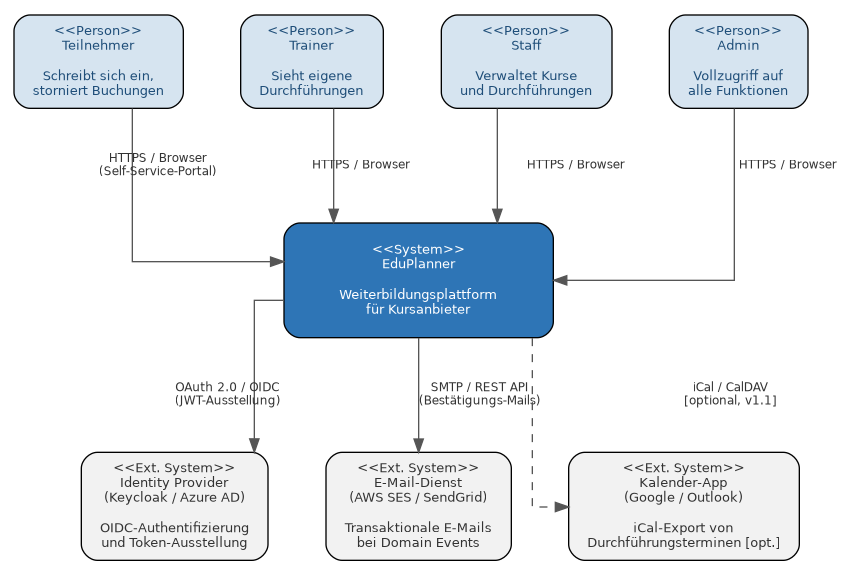
\includegraphics[width=\textwidth]{assets/context_diagram}
  \caption{\textit{C4 - Kontext Diagramm EduPlanner}}
  \label{fig:context_diagram}
\end{figure}

\subsection{Technischer Kontext}

\emph{Diagrammtyp: C4 Container Diagram.} Schichten:
\begin{enumerate}[leftmargin=2em]
  \item \textbf{Client:}
  Angular~SPA oder Vue.js~SPA (TypeScript) im Browser.
  \item \textbf{API Gateway:}
  Spring Cloud Gateway oder NGINX --
  TLS-Terminierung, Rate-Limiting, JWT-Weiterleitung.
  \item \textbf{Services:}
  catalog, scheduling, registration, notification,
  identity -- je in eigenem Kubernetes-Pod.
  \item \textbf{Datenhaltung:}
  Je eine PostgreSQL-Datenbank pro Service;
  RabbitMQ für asynchrone Events.
\end{enumerate}


\subsubsection{Technische Protokolle}

\begin{tabularx}{\textwidth}{L{4cm} L{2.8cm} X}
  \rowcolor{tableheader}
  \color{white}\textbf{Verbindung} & \color{white}\textbf{Protokoll} & \color{white}\textbf{Bemerkung} \\
  SPA $\to$ API Gateway & HTTPS / TLS & Port 443; REST APIs via JSON \\
  \rowcolor{tablegrey}
  Gateway $\to$ Services & HTTP / JSON & Internes K8s-Netzwerk; JWT-Header-Propagierung \\
  Services $\to$ DB & JDBC & PostgreSQL-Protokoll; Port 5432 \\
  \rowcolor{tablegrey}
  Services $\to$ RabbitMQ & AMQP & Port 5672; asynchrone Domain Events \\
  System $\to$ E-Mail & SMTP/REST & Verschlüsselt via STARTTLS oder REST-API \\
  \rowcolor{tablegrey}
  System $\to$ IdP & OIDC/OAuth~2.0 & HTTPS-Endpunkte für Token-Validation und UserInfo \\
  API-Spezifikation & OpenAPI~3.1.0 & Contract-First: Spec in \texttt{openapi/}\allowbreak \texttt{eduplanner-}\allowbreak \texttt{api.yaml};
  Swagger~UI je Service unter \texttt{/swagger-ui/index.html};
  vollständige Übersicht in Anhang~D (ADR-011). \\
\end{tabularx}

\subsection{Systemabgrenzung (Out-of-Scope)}

\begin{reviewbox}[Systemgrenze in einem Satz]
EduPlanner verwaltet Kurskatalog, Durchführungsplanung, Einschreibung,
Benachrichtigung und Identitätsanbindung -- \textbf{nicht} aber
Lerninhalte, Zahlungsflüsse oder die Passwortverwaltung der Nutzer.
\end{reviewbox}

Was EduPlanner \textbf{nicht} leistet (Explizite Abgrenzung nach arc42~v9):

\begin{tabularx}{\textwidth}{L{4cm} X}
  \rowcolor{tableheader}
  \color{white}\textbf{Nicht im Scope} &
  \color{white}\textbf{Begründung / Verweis} \\

  Lerninhalt (LMS) &
  EduPlanner verwaltet Kurse und Buchungen -- kein
  Moodle-Ersatz. Inhalte (Videos, Lernmaterial) liegen
  extern. LMS-Integration geplant für v2.0
  (Kap.~14). \\

  \rowcolor{tablegrey}
  Zahlungsabwicklung &
  Integration einer Zahlungsabwicklung wie z.\,B.\ Stripe
  erst in v2.0 (Kap.~14). Rechnungsstellung und
  Zahlungsflüsse sind kein MVP-Scope. \\

  Identity Management &
  Passwortverwaltung, MFA-Setup\footnotemark{} und
  User-Provisioning liegen vollständig beim externen
  IdP (ADR-003). \\

  \rowcolor{tablegrey}
  Videokonferenz / Streaming &
  Keine Integration von Zoom, MS-Teams o.\,ä.\
  Durchführungen können physisch oder extern gelinkt
  sein. \\

  Multi-Tenancy (v1.0) &
  Kursanbieter-Mandantentrennung erst ab v2.0
  (ADR-008, TS4). \\

  \rowcolor{tablegrey}
  Mobile App &
  Native iOS/Android-App erst in v2.0. v1.0: Responsive
  Web via gegebene SPA (Angular oder Vue.js). \\
\end{tabularx}

\footnotetext{%
  \textbf{MFA -- Multi-Factor Authentication}
  (Mehr-Faktor-Authentifizierung). Bei MFA muss sich ein
  Benutzer mit mindestens zwei unabhängigen Faktoren ausweisen,
  z.\,B.\ Passwort (Wissen) und Einmalcode per
  Authenticator-App (Besitz). \textbf{MFA-Setup} bezeichnet
  die erstmalige Einrichtung dieser zusätzlichen Faktoren --
  etwa das Verknüpfen einer Authenticator-App oder das
  Hinterlegen einer Mobilnummer für SMS-Codes. Im Kontext
  von EduPlanner liegt dieser gesamte Prozess beim externen
  Identity Provider und ist daher nicht Teil des eigenen
  Funktionsumfangs.%
}


\newpage
\section{Lösungsstrategie}
\label{sec:loesungsstrategie}

Dieses Kapitel beschreibt die grundlegenden Architekturentscheidungen
und Lösungsansätze. Detaillierte Begründungen finden sich in den ADRs
(Kap.~9).

\subsection{Kernarchitekturentscheidung}
\label{sec:kernarchitekturentscheidung}

EduPlanner folgt einer
\textbf{Microservice-Architektur}\footnotemark{},
ausgerichtet an den fünf fachlichen
Bounded~Contexts\footnotemark{}
aus dem Domain-Driven Design (DDD).
Jeder Bounded Context wird als eigenständiger Dienst mit eigener
Datenbank (Database-per-Service-Pattern) implementiert.
$\to$ Vollständige Begründung: ADR-001.

\addtocounter{footnote}{-2}
\stepcounter{footnote}
\footnotetext{%
  \textbf{Microservice-Architektur.}
  Ein Architekturstil, bei dem eine Anwendung als Sammlung kleiner,
  eigenständiger Dienste (\emph{Services}) realisiert wird. Jeder
  Service ist unabhängig deploybar, besitzt einen eigenen
  Datenhaushalt und kommuniziert mit anderen Services über
  wohldefinierte Schnittstellen (typischerweise REST oder
  asynchrone Nachrichten). Im Gegensatz zum monolithischen Ansatz
  lassen sich einzelne Services unabhängig skalieren, aktualisieren
  und durch verschiedene Teams weiterentwickeln.
  Vgl.\ Sam Newman, \emph{Building Microservices}, O'Reilly, 2021.%
}

\stepcounter{footnote}
\footnotetext{%
  \textbf{Bounded Context (Domain-Driven Design).}
  Ein \emph{Bounded Context} ist ein zentrales Konzept aus dem
  Domain-Driven Design (DDD) von Eric Evans. Er definiert eine
  explizite Grenze, innerhalb derer ein bestimmtes Domänenmodell
  mit einer einheitlichen Fachsprache (\emph{Ubiquitous Language})
  gilt. Ausserhalb dieser Grenze können dieselben Begriffe eine
  andere Bedeutung haben -- z.\,B.\ meint ``Kurs'' im Context
  \texttt{catalog} die inhaltliche Beschreibung, im Context
  \texttt{scheduling} hingegen eine konkrete Durchführung mit
  Datum und Ort.
  Bounded Contexts bilden in einer Microservice-Architektur die
  natürlichen Dienstgrenzen: ein Service pro Bounded Context.
  Vgl.\ Eric Evans, \emph{Domain-Driven Design}, Addison-Wesley,
  2003.%
}

\subsubsection{Microservices vs. Modularer Monolith -- Faire Gegenüberstellung}

\begin{reviewbox}[Didaktische Anmerkung]
Die Entscheidung für Microservices ist bei kleinem Team und engem MVP-Scope nicht
selbstverständlich. Nachfolgend eine explizite Gegenüberstellung beider Optionen --
denn für EduPlanner wäre ein modularer Monolith zunächst die \emph{einfachere}
Wahl gewesen.
\end{reviewbox}

\begin{tabularx}{\textwidth}{L{4cm} X X}
  \rowcolor{tableheader}
  \color{white}\textbf{Kriterium} &
  \color{white}\textbf{Modularer Monolith} &
  \color{white}\textbf{Microservices (gewählt)} \\
  Betriebskomplexität &
  Gering: 1~Prozess, 1~Datenbank, 1~Deployment-Artefakt. &
  Hoch: 5~Services, 5~Datenbanken, Message Broker, API Gateway. \\
  \rowcolor{tablegrey}
  Lokale Entwicklung &
  Einfach: \texttt{mvn spring-boot:run} genügt. &
  Aufwändig: Docker Compose mit 8+ Containern. \\
  Skalierbarkeit &
  Immer das gesamte System; keine Teilskalierung. &
  Selektiv: \texttt{registration} zur Spitzenzeit auf 10~Pods,
  \texttt{catalog} auf 1~Pod. \\
  \rowcolor{tablegrey}
  Team-Autonomie &
  Gemeinsames Codebase; Merge-Konflikte bei paralleler Entwicklung. &
  Separate Repositories; Teams deployen unabhängig. \\
  Datenkonsistenz &
  ACID-Transaktionen über Modulgrenzen hinweg. &
  Nur Eventual Consistency; Saga-Muster für verteilte Transaktionen. \\
  \rowcolor{tablegrey}
  Einstiegshürde &
  Niedrig: Standard-Wissen reicht. &
  Hoch: Verteilte Systeme, Netzwerkpartitionen, Observability. \\
  Technische Schulden &
  Modulgrenzen erodieren mit der Zeit (``Big Ball of Mud''). &
  Service-Grenzen sind hart; Erosion schwerer möglich. \\
  \rowcolor{tablegrey}
  Passt für EduPlanner? &
  Ja -- für MVP und kleine Teamgrösse sogar naheliegender. &
  Ja -- wenn Skalierbarkeit und Team-Autonomie langfristig wichtiger
  sind als kurzfristige Einfachheit. \\
\end{tabularx}

\begin{hinweis}[Warum trotzdem Microservices?]
Drei konkrete Faktoren haben den Ausschlag gegeben
(vollständige Begründung in ADR-001):
\begin{enumerate}[leftmargin=2em]
  \item \textbf{Unterschiedliche Skalierungsbedarfe:} Der
  \texttt{registration}-Service muss zur Einschreibungsfrist horizontal
  skalieren; \texttt{catalog} und \texttt{notification} haben einen
  Bruchteil der Last. Im Monolithen wäre nur vertikale Skalierung des
  Gesamtsystems möglich.
  \item \textbf{Klare fachliche Grenzen:} Die fünf Bounded Contexts haben
  grundlegend verschiedene Änderungsraten (Katalog ändert sich selten,
  Einschreibungslogik häufig). Getrennte Deployments vermeiden, dass ein
  stabiles Modul wegen Änderungen an einem anderen neu deployt wird.
  \item \textbf{Lernziel der Unterrichtsunterlage:} Microservices sind
  in der Praxis weit verbreitet; die Dokumentation zeigt Studierenden
  ein realistisches Architekturmuster mit seinen echten Trade-offs
  (vgl.\ ATAM-light, Kap.~10.1).
\end{enumerate}
\textbf{Modularer Monolith als Fallback:} Falls der Betriebsaufwand das
Team überfordert, ist ein Rückbau auf einen modularen Monolithen explizit
als Risikomitigierung geplant (Risiko R5, Kap.~11).
\end{hinweis}

% ──────────────────────────────────────────────
\subsection{Fachliche Strategie (Domain-Driven Design)}

\begin{enumerate}[leftmargin=2em]

  \item \textbf{Event~Storming} (nach Alberto Brandolini) als
  kollaborative Methode zur Domänenentdeckung.
  Dabei modellieren Fachexperten und Entwickler gemeinsam
  mit Hilfe eines Whiteboards den gesamten Geschäftsprozess -- ausgehend
  von \emph{Ereignissen} (``Teilnehmer hat sich
  eingeschrieben'', ``Kurs wurde veröffentlicht'' etc.).
  Aus den entdeckten Ereignissen lassen sich natürliche
  fachliche Grenzen ableiten, die direkt in die
  Bounded-Context-Struktur einfliessen.
  Das Event-Storming-Ergebnis für EduPlanner ist in
  Anhang~A dokumentiert.

  \item \textbf{5~Bounded Contexts} als natürliche Dienstgrenzen.
  EduPlanner definiert fünf Kontexte mit klarer fachlicher
  Verantwortlichkeit: \texttt{catalog},
  \texttt{scheduling}, \texttt{registration},
  \texttt{notification} und \texttt{identity}.
  Die Kontextgrenzen wurden im Event Storming identifiziert
  und decken sich bewusst 1:1 mit den Servicegrenzen
  (Details siehe Abschnitt~4.2.1).

  \item \textbf{Ubiquitous Language} (allgegenwärtige Sprache)
  je Kontext. Jeder Bounded Context pflegt ein eigenes,
  verbindliches Vokabular, das sowohl im Fachgespräch als
  auch im Quellcode (Klassen, Methoden, Events) konsistent
  verwendet wird. Dadurch wird sichergestellt, dass
  Missverständnisse zwischen Fachseite und Entwicklung
  minimiert werden. Das vollständige Glossar pro Context
  findet sich in Kap.~12.

  \item \textbf{Domain Events} als primäres Muster der
  kontextübergreifenden Kommunikation.
  Wenn in einem Bounded Context ein fachlich relevantes
  Ereignis eintritt (z.\,B.\
  \texttt{EnrollmentConfirmed}), wird dieses als
  \emph{Domain Event} über den Message Broker
  (RabbitMQ) veröffentlicht. Andere Contexts können
  dieses Event abonnieren und darauf reagieren -- etwa
  der \texttt{notification}-Context, der daraufhin eine
  Bestätigungsmail versendet. Dieses Muster entkoppelt
  die Services: Der sendende Context muss nicht wissen,
  wer das Event konsumiert.

  \item \textbf{Aggregate} als Konsistenzgrenzen.
  Ein Aggregate ist eine Gruppe fachlich zusammengehöriger
  Objekte, die immer gemeinsam geladen, validiert und
  gespeichert werden. Jedes Aggregate besitzt genau einen
  \emph{Aggregate Root} -- das ist der einzige
  Einstiegspunkt von aussen. Beispiel: Im Context
  \texttt{registration} bildet die Einschreibung
  (\texttt{Enrollment}) das Aggregate Root; die
  zugehörigen Wartelisteneinträge und
  Stornierungsinformationen sind Teil desselben
  Aggregates und können nur über das Root verändert
  werden. So wird sichergestellt, dass Geschäftsregeln
  (z.\,B.\ ``maximale Teilnehmerzahl'') bei jeder
  Änderung konsistent geprüft werden.

\end{enumerate}

% ──────────────────────────────────────────────
\subsubsection{Bounded Contexts und Verantwortlichkeiten}

Die folgende Tabelle ordnet jedem Bounded Context seine fachliche
Verantwortlichkeit zu. Die Spalte \emph{ADRs} verweist auf die
Architekturentscheidungen (Kap.~9), die den jeweiligen Context
massgeblich beeinflusst haben -- etwa hinsichtlich Serviceschnitt,
Kommunikationsmuster oder Datenhaltung.

\begin{tabularx}{\textwidth}{L{2.5cm} X L{2.5cm}}
  \rowcolor{tableheader}
  \color{white}\textbf{Bounded Context} &
  \color{white}\textbf{Verantwortlichkeit} &
  \color{white}\textbf{Relevante ADRs} \\

  \texttt{catalog} &
  Kursbeschreibungen, Lernziele, Trainer-Profile.
  Definiert \emph{was} angeboten wird. &
  ADR-001, ADR-006 \\

  \rowcolor{tablegrey}
  \texttt{scheduling} &
  Durchführungen, Termine, Kapazitäten,
  Trainer-Zuweisung. Definiert \emph{wann} und
  \emph{wie}. &
  ADR-001, ADR-006 \\

  \texttt{registration} &
  Einschreibungen, Warteliste, Kapazitätsprüfung,
  Stornierungen. Verwaltet \emph{wer}. &
  ADR-001, ADR-004, ADR-006 \\

  \rowcolor{tablegrey}
  \texttt{notification} &
  Event-getriebener Versand von
  E-Mail-Benach\-richtigun\-gen. &
  ADR-001, ADR-002 \\

  \texttt{identity} &
  Authentifizierung, Rollenmanagement,
  OIDC-Integration. &
  ADR-001, ADR-003 \\
\end{tabularx}


% ──────────────────────────────────────────────
\subsubsection{DDD Context Map -- Beziehungen zwischen Bounded Contexts}

Die Context~Map zeigt, wie die fünf Bounded Contexts miteinander
interagieren. Jede Beziehung folgt einem etablierten
\emph{Beziehungsmuster} aus dem Domain-Driven Design. Diese Muster
beschreiben, wie zwei Contexts miteinander kommunizieren und wer
dabei die Hoheit über das Datenmodell hat.

\begin{figure}[H]
  \centering
  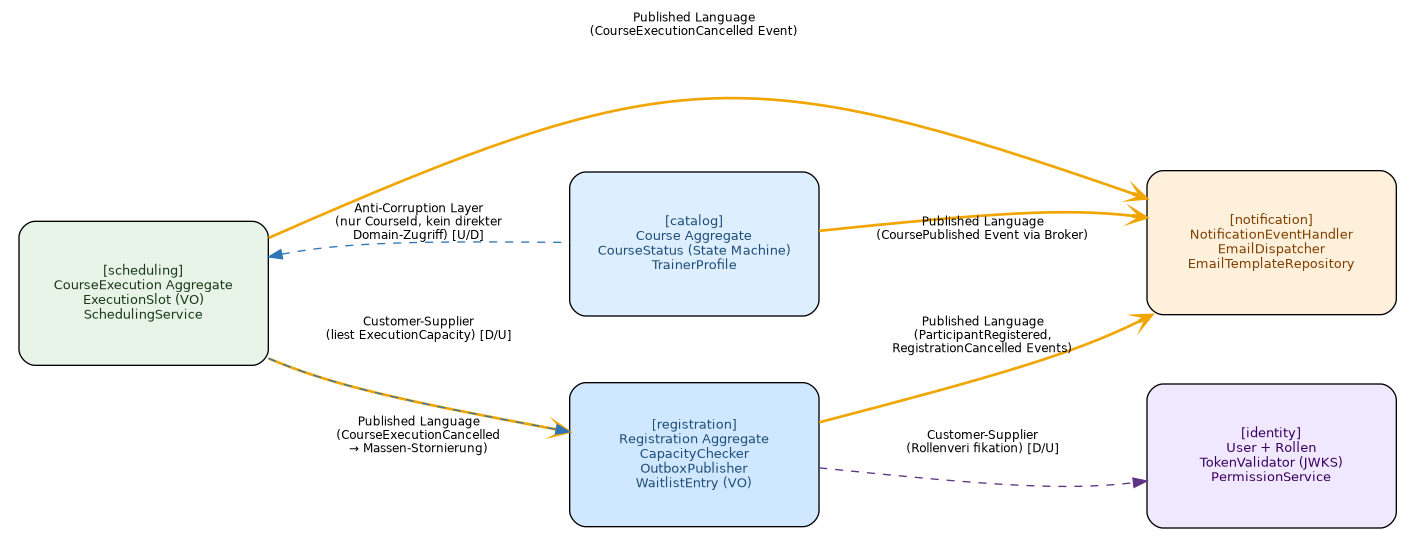
\includegraphics[width=\textwidth]{assets/context_map}
  \caption{\textit{DDD Context Map: Bounded Contexts und Beziehungen}}
  \label{fig:context_map}
\end{figure}

\begin{tabularx}{\textwidth}{L{3.5cm} L{3cm} X}
  \rowcolor{tableheader}
  \color{white}\textbf{Beziehung} &
  \color{white}\textbf{Muster (DDD)} &
  \color{white}\textbf{Erläuterung} \\

  scheduling $\leftrightarrow$ catalog &
  Anti-Corruption Layer\,(ACL) &
  Ein ACL ist eine Schutzschicht, die verhindert, dass
  das Domänenmodell eines fremden Contexts in den eigenen
  Code ``hineinwächst''. Konkret: \texttt{scheduling}
  übernimmt \emph{keine} Klassen oder Strukturen aus
  \texttt{catalog}, sondern übersetzt eingehende Daten
  an der Grenze in eigene Objekte. Es wird lediglich die
  \texttt{CourseId} als Referenz verwendet -- nie das
  vollständige Kursmodell. So bleibt \texttt{scheduling}
  unabhängig, selbst wenn sich das Modell in
  \texttt{catalog} ändert. \\

  \rowcolor{tablegrey}
  registration $\to$ scheduling &
  Customer-Supplier &
  In diesem Muster gibt es eine klare Rollenverteilung:
  Der \emph{Supplier} (Lieferant) stellt eine
  Schnittstelle bereit, der \emph{Customer} (Kunde)
  konsumiert sie. Hier liefert \texttt{scheduling} als
  Supplier Kapazitätsdaten (z.\,B.\ freie Plätze) über
  eine synchrone REST-API. \texttt{registration} als
  Customer ruft diese Daten ab, um bei einer
  Einschreibung zu prüfen, ob noch Plätze verfügbar
  sind. Der Supplier verpflichtet sich, die
  Schnittstelle stabil zu halten. \\

  registration $\to$ identity &
  Customer-Supplier &
  Gleiche Rollenverteilung: \texttt{identity} ist
  Supplier und stellt das Berechtigungsmodell bereit
  (Rollen, Berechtigungen). \texttt{registration} als
  Customer fragt bei Bedarf Rollendaten ab -- etwa um
  zu entscheiden, ob ein Nutzer eine Einschreibung
  stornieren darf. \\

  \rowcolor{tablegrey}
  catalog / reg / sched $\to$ notification &
  Published Language &
  Bei diesem Muster einigen sich die beteiligten Contexts
  auf ein \emph{gemeinsames, dokumentiertes Datenformat}
  für die Kommunikation -- hier in Form von Domain Events
  mit definierter JSON-Struktur (z.\,B.\
  \texttt{EnrollmentConfirmed}, \texttt{CoursePublished}).
  \texttt{notification} kennt \emph{aus\-schliess\-lich}
  dieses Event-Format und hat keinen Einblick in die
  internen Domänenmodelle der sendenden Contexts.
  Die Events werden asynchron über den Message Broker
  (RabbitMQ) transportiert. So kann
  \texttt{notification} eine Bestätigungsmail versenden,
  ohne zu wissen, wie eine Einschreibung intern
  modelliert ist. \\
\end{tabularx}

\subsubsection{Zusammenfassung der Architekturentscheidungen}

Die folgende Tabelle fasst die zentralen Architekturentscheidungen
zusammen, die aus der gewählten Microservice-Architektur und den
oben beschriebenen Bounded-Context-Beziehungen resultieren. Jede
Entscheidung ist in einem eigenen ADR (Kap.~9) ausführlich
dokumentiert und begründet.

\begin{tabularx}{\textwidth}{L{3.5cm} X L{2cm}}
  \rowcolor{tableheader}
  \color{white}\textbf{Entscheidung} &
  \color{white}\textbf{Begründung} &
  \color{white}\textbf{ADR} \\

  Microservices &
  Unabhängige Deployments, Team-Autonomie,
  horizontale Skalierung &
  ADR-001 \\

  \rowcolor{tablegrey}
  Database per Service &
  Verhindert Kopplung auf DB-Ebene; unabhängige
  Schema-Migrationen &
  ADR-001, ADR-006 \\

  REST + JSON &
  Standardprotokoll, breite Toolunterstützung &
  ADR-005 \\

  \rowcolor{tablegrey}
  Asynchrones Messaging &
  Entkopplung; Resilienz bei Teilausfällen &
  ADR-002 \\

  Transactional Outbox &
  Atomare Event-Persistenz; verhindert
  Dual-Write-Problem &
  ADR-004, ADR-009 \\

  \rowcolor{tablegrey}
  Container / Kubernetes &
  Einheitliches Deployment, Auto-Scaling,
  Cloud-Portabilität &
  ADR-001 \\

  Externer OIDC-IdP &
  Security-Best-Practices, MFA,
  DSGVO-Compliance &
  ADR-003 \\

  \rowcolor{tablegrey}
  Angular / Vue.js SPA &
  Reaktive UX; bekanntes Ökosystem im Team &
  ADR-005 \\
\end{tabularx}


% ──────────────────────────────────────────────
\subsection{Übergreifende Architekturprinzipien}

Die folgenden Prinzipien sind die nicht-verhandelbaren Leitlinien
der EduPlanner-Architektur. Sie gelten serviceübergreifend und
dienen als Entscheidungsrahmen im Entwicklungsalltag: Wann immer
eine Design-Frage aufkommt, geben diese Prinzipien die Richtung
vor. Einzelne Architekturentscheidungen (Kap.~9) lassen sich
jeweils auf eines oder mehrere dieser Prinzipien zurückführen.

\begin{itemize}[leftmargin=1.5em]
  \item \textbf{Favour Async over Sync:}
  Zustandsändernde Operationen zwischen Bounded Contexts
  erfolgen ausschliesslich via Domain Events. Synchrone
  REST-Aufrufe nur für lesende Operationen.
  \item \textbf{No Shared Databases:}
  Kein direkter Cross-Service-Datenbankzugriff.
  \item \textbf{Fail Fast, Recover Gracefully:}
  Transiente Fehler durch Retry + Exponential Backoff.
  Nicht-kritische Ausfälle (z.\,B.\ \texttt{notification})
  blockieren nie den Kernprozess.
  \item \textbf{Security by Default:}
  JSON-Web-Token-Validierung (JWT) am Gateway;
  zusätzliche rollenbasierte Zugriffskontrolle
  (Role-Based Access Control, RBAC) in jedem Service.
  \item \textbf{Privacy by Design:}
  Keine personenbezogenen Daten (Personally Identifiable
  Information, PII) in Logs, Events oder Metriken. Events
  referenzieren ausschliesslich \texttt{userId}, nie
  E-Mail-Adresse oder Name.
  \item \textbf{Explizite Architekturentscheidungen:}
  Jede signifikante Entscheidung wird als Architecture
  Decision Record (ADR) dokumentiert.
\end{itemize}


% ──────────────────────────────────────────────
\subsection{Qualitätsziel-Mapping}

Jede Architekturentscheidung in EduPlanner dient mindestens einem
übergeordneten Qualitätsziel. Die folgende Tabelle macht diesen
Zusammenhang explizit: Sie ordnet den zentralen Qualitätszielen
nach ISO~25010\footnotemark{} die jeweils wichtigsten
Architekturmassnahmen zu. So wird nachvollziehbar, \emph{warum}
bestimmte Muster und Technologien gewählt wurden -- und welche
Kapitel die jeweilige Massnahme im Detail beschreiben.

\footnotetext{%
  \textbf{ISO~25010} ist ein internationaler Standard, der ein
  Qualitätsmodell für Softwareprodukte definiert. Er gliedert
  Qualität in acht Hauptmerkmale -- darunter Funktionalität,
  Zuverlässigkeit, Sicherheit, Wartbarkeit und Benutzbarkeit.
  Das Modell dient als gemeinsame Sprache, um Qualitätsanforderungen
  messbar und vergleichbar zu formulieren.%
}

\begin{tabularx}{\textwidth}{L{4cm} X L{2cm}}
  \rowcolor{tableheader}
  \color{white}\textbf{Qualitätsziel (ISO~25010)} &
  \color{white}\textbf{Architekturmassnahme} &
  \color{white}\textbf{Referenz} \\

  Functional Correctness &
  \emph{Optimistic Locking} stellt sicher, dass parallele
  Änderungen an denselben Daten (z.\,B.\ zwei gleichzeitige
  Einschreibungen auf den letzten Platz) erkannt und
  konfliktfrei aufgelöst werden. Alle Schreiboperationen
  erfolgen transaktional. Event-Handler sind
  \emph{idempotent} -- d.\,h.\ ein mehrfach empfangenes
  Event führt nicht zu doppelten Einschreibungen. &
  Kap.~5.4, 8.4 \\

  \rowcolor{tablegrey}
  Reliability -- Availability &
  Kubernetes \emph{Health-Probes} (Liveness / Readiness)
  erkennen ausgefallene Pods und starten sie automatisch
  neu. \emph{Circuit Breaker} (via Resilience4j) verhindern,
  dass der Ausfall eines Services sich kaskadenartig auf
  andere ausbreitet. Die PostgreSQL-Datenbanken laufen
  redundant; der Message Broker (RabbitMQ) wird als Cluster
  betrieben. &
  Kap.~8.2, 7.4 \\

  Maintainability &
  Die strikten Bounded-Context-Grenzen sorgen dafür, dass
  Änderungen an einem Service keine Seiteneffekte in
  anderen Services verursachen. Kein Service greift direkt
  auf die Datenbank eines anderen zu. Alle architekturrelevanten
  Entscheidungen sind in ADRs (Kap.~9) festgehalten, sodass
  das Projektteam auch Monate später nachvollziehen kann,
  \emph{warum} etwas so entschieden wurde. &
  Kap.~5, 9 \\

  \rowcolor{tablegrey}
  Security &
  JSON Web Tokens (JWT) werden am API-Gateway validiert;
  jeder Service führt zusätzlich eine eigene rollenbasierte
  Zugriffskontrolle (RBAC) durch. Sämtliche Kommunikation
  läuft über HTTPS/TLS. In Logs, Events und Metriken werden
  keine personenbezogenen Daten (PII) gespeichert. &
  Kap.~8.1, 8.2 \\

  Usability &
  Die Single-Page-Application (Angular oder Vue.js) bietet
  eine reaktive Benutzeroberfläche ohne Seitenwechsel.
  Formulare sind auf minimale Eingaben optimiert.
  \emph{Progressive Loading} lädt nur die aktuell benötigten
  Inhalte nach, um die wahrgenommene Ladezeit zu reduzieren.
  Der Mobile-First-Ansatz stellt sicher, dass das Interface
  auch auf Smartphones nutzbar ist. &
  ADR-005 \\
\end{tabularx}

% ──────────────────────────────────────────────
\subsection{Skalierungsstrategie pro Bounded Context}

Nicht alle Services von EduPlanner sind gleich stark belastet.
Der \texttt{registration}-Service erlebt beispielsweise zu
Einschreibungsfristen hohe Lastspitzen, während \texttt{catalog}
überwiegend Lesezugriffe bedient. Deshalb wird jeder Service
individuell skaliert.

Die Skalierung erfolgt automatisiert über den Kubernetes
\emph{Horizontal Pod Autoscaler} (HPA): Sobald ein definierter
Schwellenwert (\emph{Scale-Trigger}) überschritten wird, startet
Kubernetes zusätzliche Pod-Instanzen des betroffenen Services --
bis zur konfigurierten Obergrenze. Fällt die Last wieder, werden
überschüssige Pods abgebaut. Die Spalten \emph{Min~Pods} und
\emph{Max~Pods} definieren den Skalierungskorridor pro Service.

\begin{tabularx}{\textwidth}{L{3cm} C{2cm} C{2cm} X}
  \rowcolor{tableheader}
  \color{white}\textbf{Service} &
  \color{white}\textbf{Min~Pods} &
  \color{white}\textbf{Max~Pods} &
  \color{white}\textbf{Scale-Trigger} \\

  registration & 2 & 10 &
  CPU-Auslastung $>$ 70\,\% oder
  Warteschlangentiefe $>$ 100~Nachrichten \\

  \rowcolor{tablegrey}
  catalog & 1 & 3 &
  CPU-Auslastung $>$ 80\,\%
  (primär Lesezugriffe) \\

  scheduling & 2 & 5 &
  CPU-Auslastung $>$ 70\,\% \\

  \rowcolor{tablegrey}
  notification & 1 & 10 &
  Warteschlangentiefe $>$ 500~Nachrichten \\

  identity & 2 & 5 &
  Antwortzeit (Request-Latency) $>$ 200\,ms \\
\end{tabularx}

\newpage
\section{Bausteinsicht}
\label{sec:bausteinsicht}

Die Bausteinsicht zeigt die statische Zerlegung des Systems in
seine Bausteine (Services, Komponenten, Klassen) sowie deren
Abhängigkeiten. Sie beantwortet die Frage: \emph{Aus welchen
Teilen besteht EduPlanner und wie hängen diese zusammen?}

Die Darstellung folgt dem \textbf{Zoom-in-Prinzip} des
arc42-Templates: Ebene~1 zeigt das Gesamtsystem als Whitebox
mit seinen fünf Services und der Infrastruktur. Die Ebenen~2
und~3 zoomen schrittweise in einzelne Bounded Contexts hinein
-- bis hin zu kritischen Klassen und Algorithmen.

Für die Diagramme wird die \textbf{C4-Notation}\footnotemark{}
verwendet. Jede Ebene enthält zunächst ein Diagramm zur
Orientierung, gefolgt von einer Tabelle bzw.\ Auflistung mit
den Verantwortlichkeiten der dargestellten Bausteine.

\footnotetext{%
  \textbf{C4-Modell} (nach Simon Brown). Ein hierarchisches
  Diagrammmodell für Softwarearchitektur mit vier
  Abstraktionsebenen: \emph{Context} (System im Umfeld),
  \emph{Container} (deploybare Einheiten), \emph{Component}
  (logische Bausteine innerhalb eines Containers) und
  \emph{Code} (Klassen/Interfaces). Jede Ebene zoomt tiefer
  in das System hinein.
  Vgl.\ \url{https://c4model.com}.%
}

% ══════════════════════════════════════════════
\subsection{Ebene~1 -- Gesamtsystem (Whitebox)}
\label{sec:baustein-ebene1}

Das folgende C4-Container-Diagramm (Abb.~\ref{fig:container})
zeigt alle deployierbaren Einheiten von EduPlanner sowie die
Kommunikationswege zwischen ihnen. Die fünf fachlichen Services
(blau) entsprechen den Bounded Contexts aus Kapitel~4.
Infrastrukturbausteine (grau) -- API Gateway, Message Broker
und Datenbanken -- sind unterstützende Komponenten ohne eigene
Fachlogik. Externe Systeme (orange) liegen ausserhalb der
Systemgrenze.

\begin{figure}[H]
  \centering
  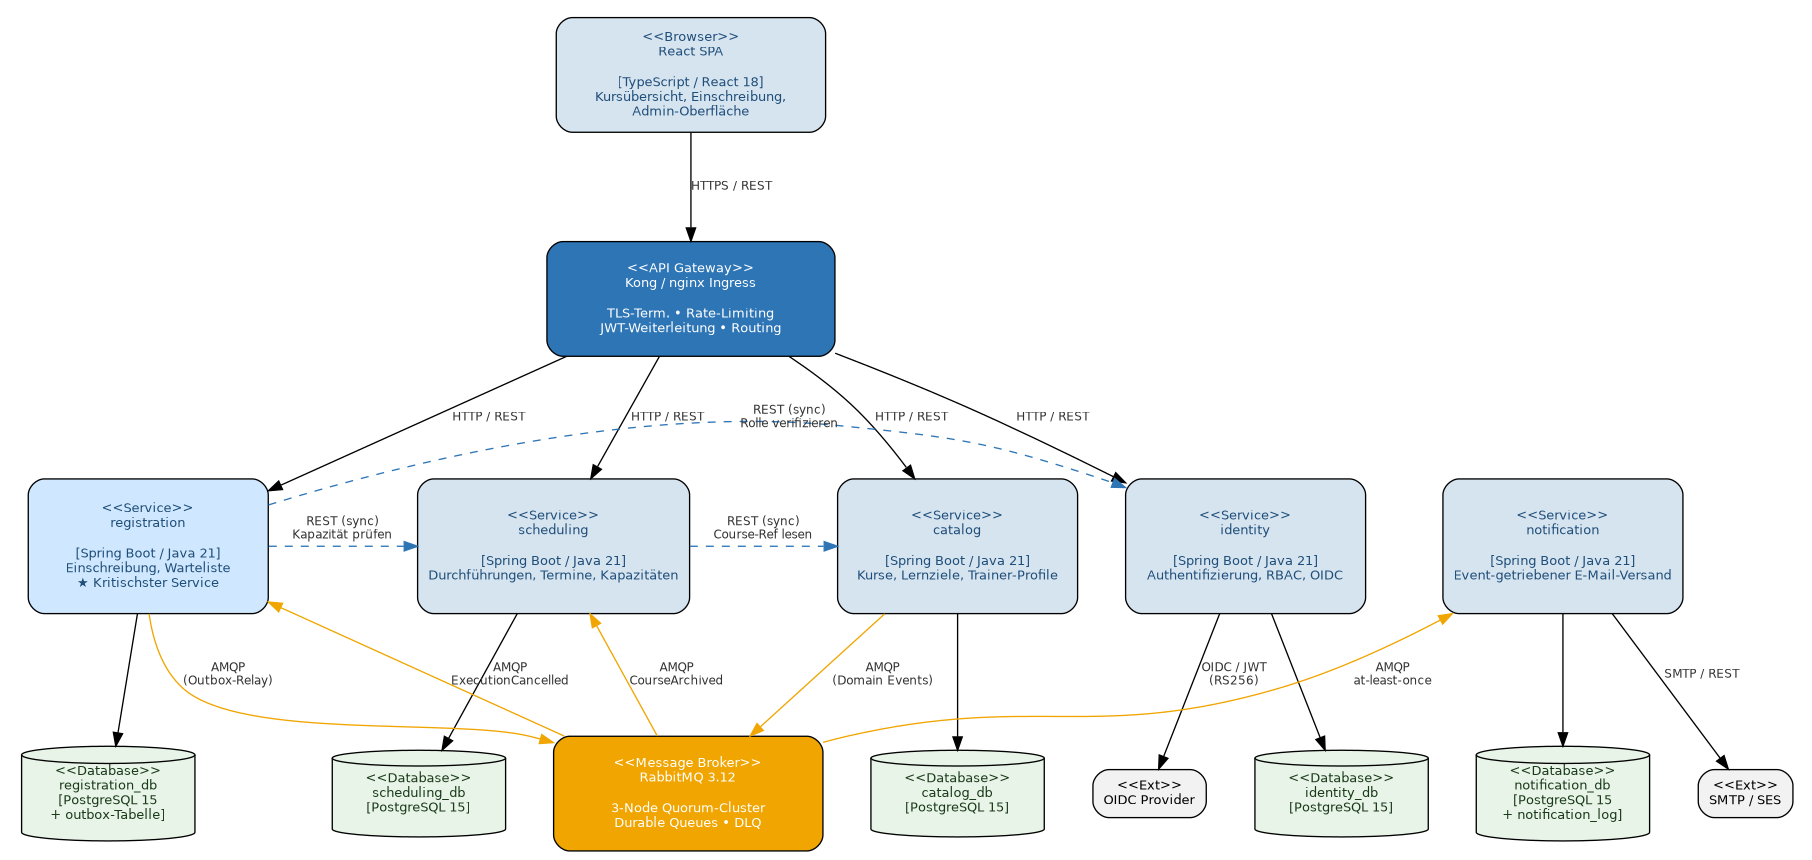
\includegraphics[width=\textwidth]{assets/ebene1_container_diagram}
  \caption{\textit{Ebene~1 -- C4-Container-Diagramm: Gesamtsystem
  EduPlanner mit Services, Infrastruktur und externen
  Systemen.}}
  \label{fig:container}
\end{figure}

Die nachfolgende Tabelle beschreibt die Verantwortlichkeit
jedes Bausteins im Detail:

\begin{tabularx}{\textwidth}{L{2.8cm} X}
  \rowcolor{tableheader}
  \color{white}\textbf{Baustein} &
  \color{white}\textbf{Verantwortlichkeit} \\

  \texttt{catalog} &
  Kursbeschreibungen, Lernziele, Trainer-Profile.
  Publiziert \texttt{CourseCreated},
  \texttt{CoursePublished},
  \texttt{CourseArchived}. \\

  \rowcolor{tablegrey}
  \texttt{scheduling} &
  Planung von Kursdurchführungen inkl.\ Termine,
  Kapazitäten, Trainer-Zuweisung. \\

  \texttt{registration} &
  Einschreibungsverwaltung: Kapazitätsprüfung,
  Warteliste, Stornierungen.
  \textbf{Kritischster Service.} \\

  \rowcolor{tablegrey}
  \texttt{notification} &
  Event-getriebener E-Mail-Versand; kein Einfluss
  auf Kernprozesse. \\

  \texttt{identity} &
  Authentifizierung via OIDC-IdP; Rollen- und
  Benutzerverwaltung. \\

  \rowcolor{tablegrey}
  API Gateway &
  TLS-Terminierung, Rate-Limiting (100~Req/s),
  JWT-Weiterleitung, Routing. \\

  Message Broker &
  Entkoppelte asynchrone Kommunikation via
  Durable Queues und Dead-Letter-Exchange. \\

  \rowcolor{tablegrey}
  Reporting (BFF) &
  v1.0: Dashboard-Daten aus \texttt{catalog} und
  \texttt{registration} separat abgefragt und im
  Frontend aggregiert (BFF-Light via Angular /
  Vue.js). v2.0: Dedizierter Reporting-Service
  geplant (Kap.~14.3). \\
\end{tabularx}

% ══════════════════════════════════════════════
\subsection{Ebene~2 -- Bounded Context: \texttt{catalog}}
\label{sec:baustein-catalog}

Der \texttt{catalog}-Service ist fachlich der einfachste
Bounded Context: Er verwaltet Kursbeschreibungen und
Trainer-Profile und steuert über eine Zustandsmaschine, welche
Kurse für Teilnehmer sichtbar sind. Abbildung~\ref{fig:catalog}
zeigt die internen Bausteine und deren Zusammenspiel -- vom
REST-Controller über die Fachlogik bis hin zur Datenbank und
Event-Publikation.

\begin{figure}[H]
  \centering
  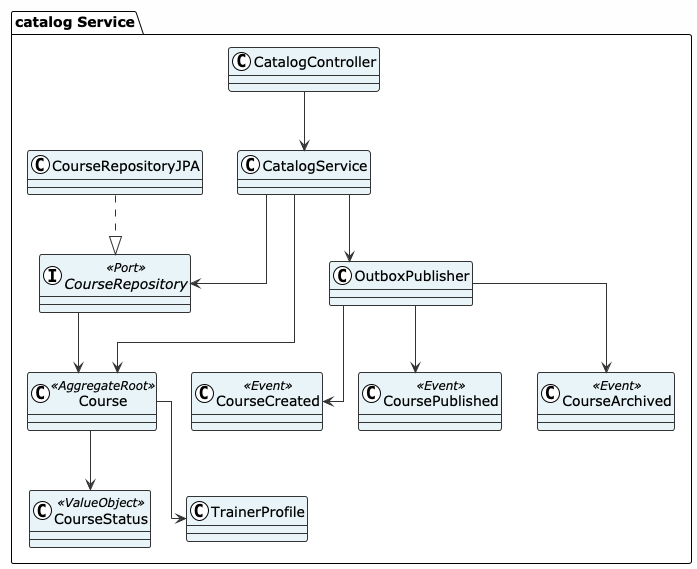
\includegraphics[width=\textwidth]{assets/ebene2_catalog_class_diagram}
  \caption{\textit{Ebene~2 -- UML-Klassendiagramm: Interne
  Bausteine des \texttt{catalog}-Service.}}
  \label{fig:catalog}
\end{figure}

Wichtige Klassen / Aggregate:
\begin{itemize}[leftmargin=1.5em]
  \item \textbf{Course} (Aggregate Root): \texttt{CourseId},
  Titel, Beschreibung, Lernziele,
  \texttt{CourseStatus}
  (Draft $\to$ Published $\to$ Archived), Trainer.
  \item \textbf{TrainerProfile}: Stammdaten, Fachgebiete,
  Verfügbarkeitsstatus.
  \item \textbf{CourseStatus}: Value Object; steuert erlaubte
  Zustandsübergänge (State Machine).
  \item \textbf{CourseRepository}: Port-Interface;
  Implementierung via JPA/Hibernate.
\end{itemize}

\noindent\textbf{Domain Events:}
\begin{itemize}[leftmargin=1.5em, label=\raisebox{0.25ex}{\tiny\(\bullet\)}]
  \item \texttt{CourseCreated} -- Neuer Kurs wurde angelegt
  \item \texttt{CoursePublished} -- Kurs wurde veröffentlicht
  \item \texttt{CourseArchived} -- Kurs wurde archiviert
\end{itemize}

% ──────────────────────────────────────────────
\subsubsection{CourseStatus -- Zustandsübergangsdiagramm}

Das \texttt{CourseStatus}-Value-Object steuert den Lebenszyklus
eines Kurses über eine einfache Zustandsmaschine mit drei
Zuständen und erlaubten Übergängen
(Abb.~\ref{fig:course-state}). Rückwärtsübergänge sind bewusst
nicht vorgesehen (ADR-006): Ein archivierter Kurs kann nicht
reaktiviert werden -- stattdessen muss ein neuer Kurs angelegt
werden.

\begin{figure}[H]
  \centering
  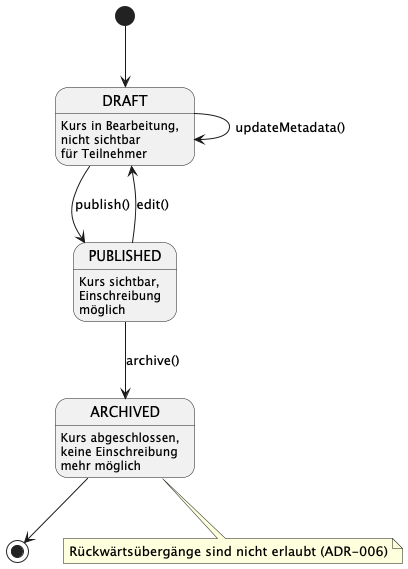
\includegraphics[width=0.55\textwidth]{assets/catalog_course_state_machine}
  \caption{\textit{Zustandsübergangsdiagramm: \texttt{CourseStatus}
  mit den drei Zuständen DRAFT, PUBLISHED und
  ARCHIVED. Rückwärtsübergänge sind nicht vorgesehen.}}
  \label{fig:course-state}
\end{figure}

% ══════════════════════════════════════════════
\subsection{Ebene~2 -- Bounded Context: \texttt{scheduling}}
\label{sec:baustein-scheduling}

Der \texttt{scheduling}-Service ist für die zeitliche und
organisatorische Planung von Kursdurchführungen verantwortlich.
Er referenziert Kurse aus \texttt{catalog} ausschliesslich über
die \texttt{CourseId} (Anti-Corruption Layer) und enthält die
kritische Logik zur Vermeidung von Trainer-Doppelbuchungen.
Abbildung~\ref{fig:scheduling} zeigt seine internen
Komponenten -- man beachte insbesondere den ACL-Baustein rechts,
der die Entkopplung vom \texttt{catalog}-Domänenmodell
sicherstellt.

\begin{figure}[H]
  \centering
  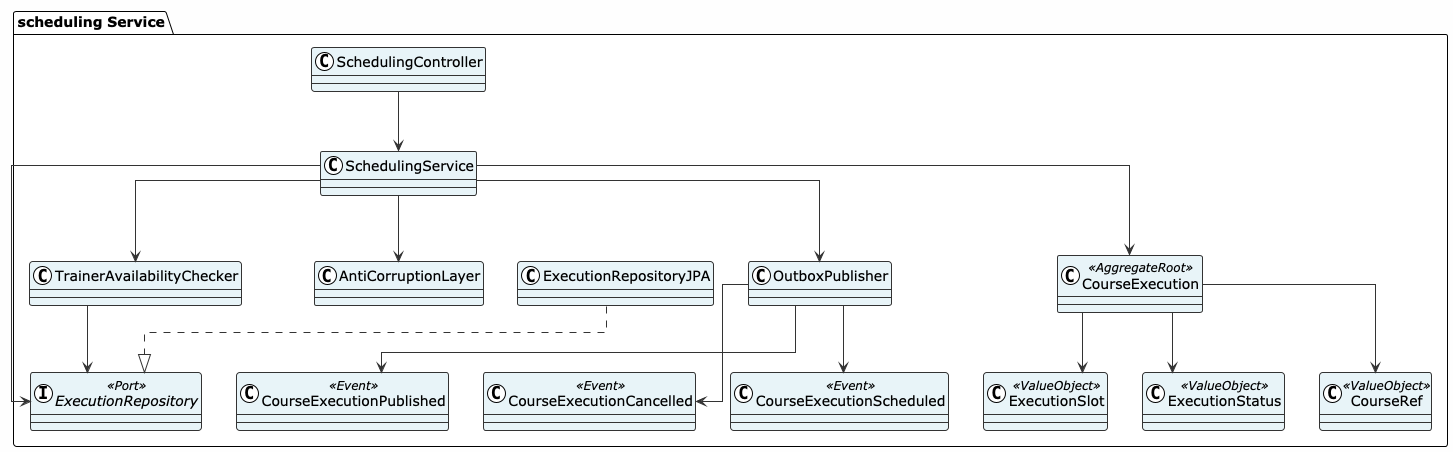
\includegraphics[width=\textwidth]{assets/ebene2_scheduling_class_diagram}
  \caption{\textit{Ebene~2 -- UML-Klassendiagramm: Interne
  Bausteine des \texttt{scheduling}-Service inkl.\
    Anti-Corruption Layer zum \texttt{catalog}-Context.}}
  \label{fig:scheduling}
\end{figure}

Wichtige Klassen / Aggregate:
\begin{itemize}[leftmargin=1.5em]
  \item \textbf{CourseExecution} (Aggregate Root):
  \texttt{CourseRef} (nur ID -- Anti-Corruption Layer),
  Startdatum, Enddatum, Ort, Kapazität,
  \texttt{ExecutionStatus}, Trainer.
  \item \textbf{SchedulingService}: Prüft
  Trainer-Verfügbarkeit und verhindert Überschneidungen.
  Die Prüflogik verwendet transaktionale Locks
  (SELECT\ldots FOR UPDATE) zur Race-Condition-Prävention
  (Details siehe Laufzeitsicht, Kap.~6).
  \item \textbf{ExecutionSlot}: Value Object für einen
  Zeitblock einer Durchführung.
\end{itemize}

\noindent\textbf{Domain Events:}
\begin{itemize}[leftmargin=1.5em, label=\raisebox{0.25ex}{\tiny\(\bullet\)}]
  \item \texttt{CourseExecutionScheduled} -- Durchführung wurde geplant
  \item \texttt{CourseExecutionPublished} -- Durchführung wurde veröffentlicht
  \item \texttt{CourseExecutionCancelled} -- Durchführung wurde abgesagt
\end{itemize}

\paragraph{Fallback-Verhalten bei Ausfall des \texttt{catalog}-Service}

Der \texttt{scheduling}-Service ist abhängig vom
\texttt{catalog}-Service, um Kursnamen zu laden. Sollte
\texttt{catalog} ausfallen oder nicht erreichbar sein, darf dies
die Kernfunktionalität von \texttt{scheduling} nicht blockieren.
Daher implementiert \texttt{scheduling} ein intelligentes
Fallback-Verhalten:

\begin{itemize}[leftmargin=1.5em]
  \item \textbf{Normale Situation}: \texttt{scheduling} ruft
  \texttt{catalog} auf und erhält den Kursnamen
  (z.\,B.\ ``Java Grundlagen'').
  \item \textbf{Ausfall von \texttt{catalog}}: Der
  \texttt{scheduling}-Service erkennt den Fehler über
  einen \textbf{Circuit Breaker} (Resilience4j). Statt
  die Anfrage zu blockieren oder zu fehlschlagen, gibt
  \texttt{scheduling} die Durchführungsdaten mit einem
  Platzhalter zurück: \texttt{[Kursinformation nicht
  verfügbar]}. Die eigentlichen Daten (Termin, Ort,
  Trainer) bleiben korrekt.
  \item \textbf{Circuit Breaker Logik}: Nach 5~Fehlern
  innerhalb von 10~Sekunden geht der Circuit Breaker in
  den Zustand ``OPEN''. Weitere Anfragen an
  \texttt{catalog} werden sofort abgelehnt, ohne zu
  warten. Nach 30~Sekunden wechselt der Circuit Breaker
  in den Zustand ``HALF-OPEN'' und versucht einen
  Testaufruf. Ist dieser erfolgreich, geht der Circuit
  Breaker zurück in den Zustand ``CLOSED''.
\end{itemize}

\textbf{Resultat:} Benutzer sehen zwar, dass Kursinformationen
temporär nicht verfügbar sind, können aber weiterhin auf
Durchführungstermine zugreifen. Dies ist ein Beispiel für
\emph{Graceful Degradation}: Das System funktioniert mit
reduzierter Funktionalität weiter, statt komplett auszufallen.

% ══════════════════════════════════════════════
\subsection{Ebene~2 -- Bounded Context: \texttt{registration}}
\label{sec:baustein-registration}

Der \texttt{registration}-Service ist der \textbf{kritischste
Bounded Context} des Systems: Er verarbeitet Einschreibungen,
verwaltet Wartelisten und muss unter allen Umständen verhindern,
dass mehr Teilnehmer eingeschrieben werden als Plätze vorhanden
sind -- auch bei hoher gleichzeitiger Last. Aus diesem Grund
ist er der einzige Service, für den eine Ebene-3-Sicht
dokumentiert wird
(siehe Abschnitt~\ref{sec:baustein-reg-ebene3}).

Abbildung~\ref{fig:registration} zeigt die internen Komponenten
inkl.\ der beiden kritischen Bausteine
\texttt{CapacityChecker} (Race-Condition-Schutz) und
\texttt{OutboxPublisher} (garantierte Event-Publikation).

\begin{figure}[H]
  \centering
  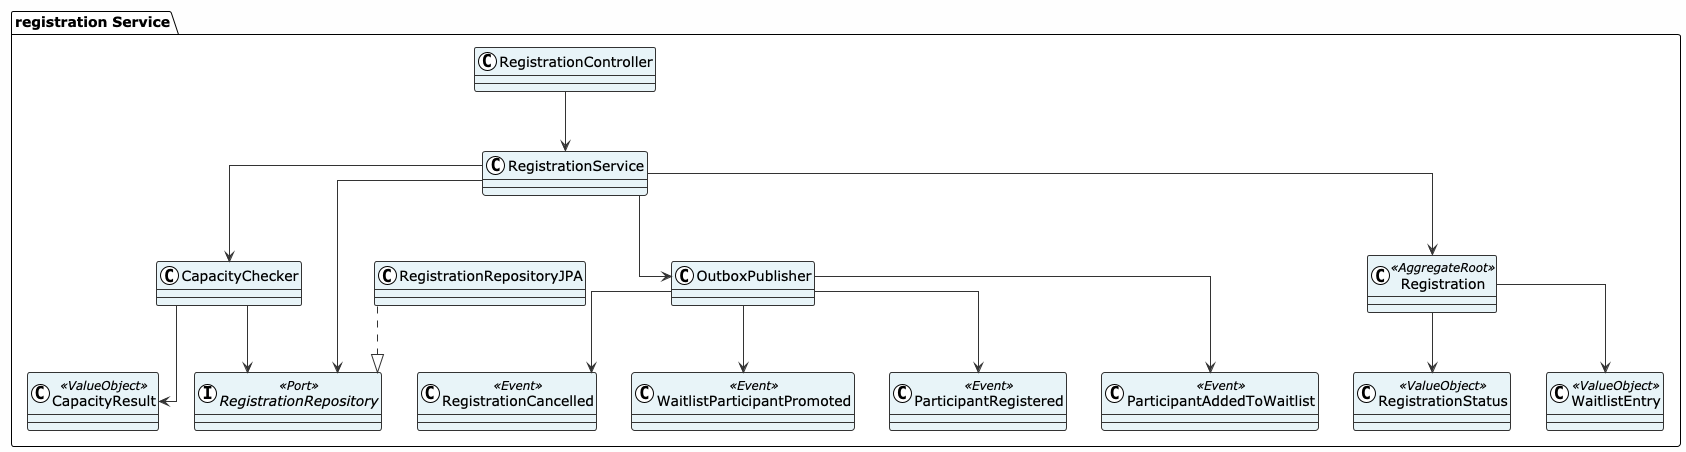
\includegraphics[width=\textwidth]{assets/ebene2_registration_class_diagram}
  \caption{\textit{Ebene~2 -- UML-Klassendiagramm: Interne
  Bausteine des \texttt{registration}-Service inkl.\
    CapacityChecker, OutboxPublisher und Anbindung an
    den Message Broker.}}
  \label{fig:registration}
\end{figure}

Wichtige Klassen / Aggregate:
\begin{itemize}[leftmargin=1.5em]
  \item \textbf{Registration} (Aggregate Root):
  \texttt{registrationId}~(UUID),
  \texttt{executionId} (ExecutionRef),
  \texttt{participantId},
  \texttt{status} (REGISTERED\,|\,CANCELLED),
  \texttt{registeredAt},
  \texttt{version}~(Long, Optimistic Locking).
  \item \textbf{CapacityChecker}: Prüft Kapazität via
  \texttt{SELECT \ldots\ FOR UPDATE} / Optimistic
  Locking. Die detaillierte Logik ist in
  Abschnitt~\ref{sec:baustein-reg-ebene3} dokumentiert.
  \item \textbf{WaitlistEntry}: Value Object mit Position
  (Integer) und Zeitstempel.
  \item \textbf{OutboxPublisher}: Schreibt Domain Events in
  die \texttt{outbox}-Tabelle innerhalb derselben
  DB-Transaktion (Transactional Outbox Pattern,
  ADR-004).
\end{itemize}

\noindent\textbf{Domain Events:}
\begin{itemize}[leftmargin=1.5em, label=\raisebox{0.25ex}{\tiny\(\bullet\)}]
  \item \texttt{ParticipantRegistered} -- Teilnehmer wurde eingeschrieben
  \item \texttt{ParticipantAddedToWaitlist} -- Teilnehmer zur Warteliste hinzugefügt
  \item \texttt{RegistrationCancelled} -- Einschreibung wurde storniert
  \item \texttt{WaitlistParticipantPromoted} -- Wartelisten-Teilnehmer wurde befördert
\end{itemize}

% ──────────────────────────────────────────────
\subsubsection{Ebene~3 -- CapacityChecker und OutboxPublisher
  (Whitebox)}
\label{sec:baustein-reg-ebene3}

Die folgenden beiden Bausteine sind die architekturkritischsten
Komponenten des gesamten Systems. Der \texttt{CapacityChecker}
stellt sicher, dass niemals mehr Einschreibungen akzeptiert
werden als Plätze vorhanden sind -- auch wenn Hunderte von
Anfragen gleichzeitig eintreffen. Der \texttt{OutboxPublisher}
garantiert, dass jedes Domain Event genau dann publiziert wird,
wenn die zugehörige Geschäftstransaktion erfolgreich war
(kein Dual-Write-Problem).

\paragraph{CapacityChecker -- Interne Logik}

Der \texttt{CapacityChecker} schützt sich vor Race Conditions
durch eine Kombination aus pessimistischen Locks und Optimistic
Locking:

\begin{lstlisting}
1. Lese Registration-Aggregate mit version-Feld:
   SELECT * FROM registrations
   WHERE execution_id = ? FOR UPDATE
   ODER: Lese via JPA @Version (Optimistic Locking)

2. Pruefe: currentCapacity > 0
   -> Einschreibung erlaubt
   -> Einschreibung abgelehnt (auf Warteliste)

3. Dekrementiere Kapazitaet; persistiere
   Registration-Entity

4. Bei OptimisticLockingFailure: Retry (max. 3x)
   mit exponentieller Backoff
\end{lstlisting}

\textbf{Szenario:} Zwei Anfragen treffen gleichzeitig ein und
versuchen, die letzte verfügbare Kapazität zu buchen. Die erste
Anfrage erwirbt den Lock via \texttt{FOR UPDATE}, dekrementiert
die Kapazität und committed. Die zweite Anfrage wartet auf den
Lock, liest dann die aktualisierte (nun leere) Kapazität und
lehnt die Einschreibung ab -- Teilnehmer wird auf Warteliste
gesetzt.

\paragraph{OutboxPublisher -- Interne Logik}

Der \texttt{OutboxPublisher} implementiert das Transactional
Outbox Pattern (ADR-004) zur garantierten Event-Publikation:

\begin{lstlisting}
1. Domain Event serialisieren (JSON)

2. INSERT INTO outbox
   (event_type, payload, status=PENDING, created_at)
   INNERHALB derselben JDBC-Transaktion wie
   die Business-Logik

3. Commit der Transaktion:
   - Entweder: Beide (Registration + Event) werden
     persistent
   - Oder: Beide werden rollback (Atomarität)

4. Separater Background-Thread (Polling):
   - Liest PENDING-Events aus der outbox-Tabelle
   - Sendet an RabbitMQ
   - Update Status -> status=SENT (oder status=FAILED)

5. Dead-Letter-Queue (DLQ):
   - Sollte ein Event nach 5 Retry-Versuchen
     noch nicht gesendet sein, landet es in der DLQ
   - Manuelle Intervention erforderlich
\end{lstlisting}

\textbf{Vorteil gegenüber Dual-Write:} Früher hätte man
zuerst die Registration in die DB schreiben und dann das Event
an RabbitMQ senden müssen. Bei Fehler zwischen diesen beiden
Operationen entsteht Inkonsistenz. Mit dem Outbox Pattern ist
beides eine atomare Operation.

% ══════════════════════════════════════════════
\subsection{Ebene~2 -- Bounded Context: \texttt{notification}}
\label{sec:baustein-notification}

Der \texttt{notification}-Service ist der einfachste Service
und hat bewusst keine fachliche Logik: Er konsumiert Domain
Events von anderen Services und versendet E-Mails. Diese
Entkopplung stellt sicher, dass E-Mail-Ausfälle den
Kernprozess (Einschreibung, Planung) nicht blockieren.
Abbildung~\ref{fig:notification} zeigt die internen Bausteine
und deren Zusammenspiel.

\begin{figure}[H]
  \centering
  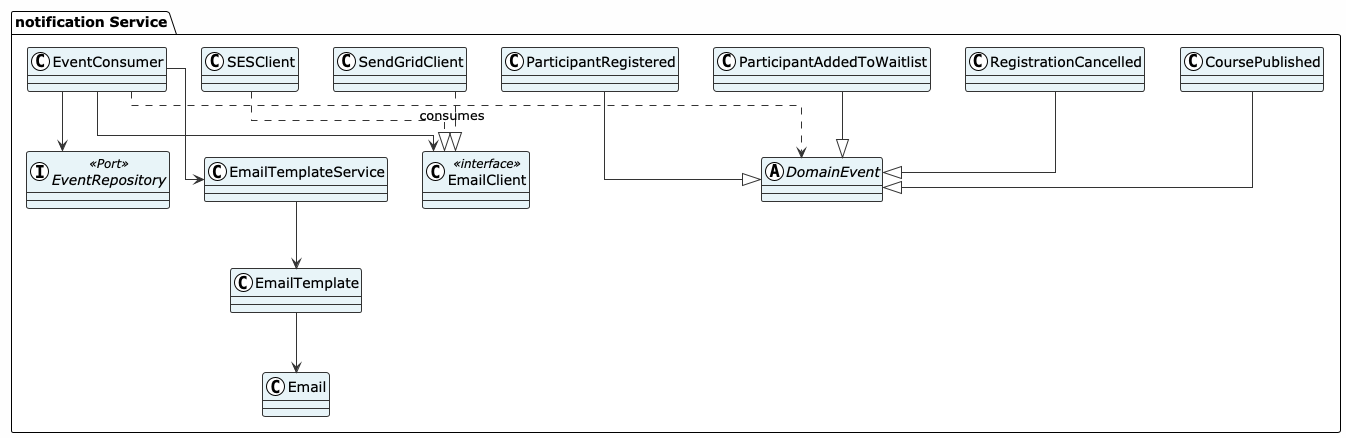
\includegraphics[width=\textwidth]{assets/ebene2_notification_class_diagram}
  \caption{\textit{Ebene~2 -- UML-Klassendiagramm: Interne
  Bausteine des \texttt{notification}-Service.}}
  \label{fig:notification}
\end{figure}

Wichtige Klassen:
\begin{itemize}[leftmargin=1.5em]
  \item \textbf{EventConsumer}: Liest Domain Events aus dem
  Message Broker (RabbitMQ) und delegiert an
  \texttt{EmailTemplateService}.
  \item \textbf{EmailTemplateService}: Wählt das passende
  Template basierend auf Event-Typ und rendert die
  E-Mail mit Event-Daten.
  \item \textbf{TemplateRegistry}: Zentrales Verzeichnis aller
  E-Mail-Templates (z.\,B.\ Bestätigung, Warteliste,
  Stornierung).
  \item \textbf{EmailClient} (Interface): Abstrahiert den
  konkreten E-Mail-Anbieter. Implementierungen:
  \texttt{SESClient} (Amazon SES) oder
  \texttt{SendGridClient} (SendGrid).
  \item \textbf{Email}: Value Object mit Empfänger, Betreff,
  HTML-Body.
\end{itemize}

\noindent\textbf{Domain Events (konsumiert):}
\begin{itemize}[leftmargin=1.5em, label=\raisebox{0.25ex}{\tiny\(\bullet\)}]
  \item \texttt{ParticipantRegistered} -- Bestätigungsmail versenden
  \item \texttt{ParticipantAddedToWaitlist} -- Wartelistenbestätigung versenden
  \item \texttt{RegistrationCancelled} -- Stornierungsbestätigung versenden
  \item \texttt{CoursePublished} -- Ankündigung an Interessenten versenden
\end{itemize}

\paragraph{Event-getriebener Versand}

Der \texttt{notification}-Service ist vollständig
\emph{event-getrieben}: Er hat keine eigene Geschäftslogik,
sondern reagiert nur auf Events, die von anderen Services
publiziert werden. Dies hat mehrere Vorteile:

\begin{itemize}[leftmargin=1.5em]
  \item \textbf{Entkopplung}: Andere Services müssen nicht
  wissen, dass E-Mails versendet werden.
  \item \textbf{Fehlertoleranz}: Sollte der
  \texttt{notification}-Service ausfallen, blockiert
  dies nicht die Einschreibung oder Planung.
  \item \textbf{Skalierbarkeit}: E-Mail-Versand ist
  zeitaufwändig. Durch asynchrone Events kann der
  Service unabhängig skaliert werden.
  \item \textbf{Wartbarkeit}: Template-Änderungen erfordern
  keine Änderungen an anderen Services.
\end{itemize}

% ══════════════════════════════════════════════
\subsection{Ebene~2 -- Bounded Context: \texttt{identity}}
\label{sec:baustein-identity}

Der \texttt{identity}-Service ist ein dünner Adapter zwischen
EduPlanner und dem externen Identity Provider (Keycloak via
OIDC). Er verwaltet keine Passwörter oder Credentials, sondern
delegiert alle Authentifizierung an den IdP und cached nur
Rollen und Berechtigungen. Abbildung~\ref{fig:identity} zeigt
die internen Bausteine und deren Zusammenspiel.

\begin{figure}[H]
  \centering
  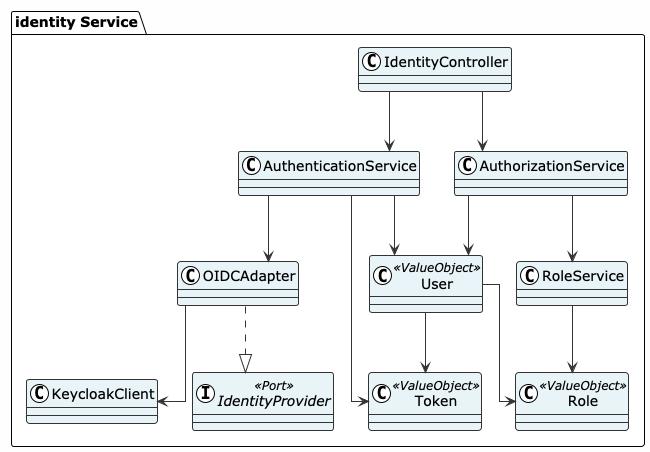
\includegraphics[width=\textwidth]{assets/ebene2_identity_class_diagram}
  \caption{\textit{Ebene~2 -- UML-Klassendiagramm: Interne
  Bausteine des \texttt{identity}-Service.}}
  \label{fig:identity}
\end{figure}

Wichtige Klassen:
\begin{itemize}[leftmargin=1.5em]
  \item \textbf{AuthenticationService}: Orchestriert den
  Authentifizierungsprozess. Delegiert an
  \texttt{OIDCAdapter} und \texttt{TokenValidator}.
  \item \textbf{OIDCAdapter}: Kommuniziert mit dem externen
  Identity Provider (Keycloak). Implementiert das
  OpenID Connect Protokoll.
  \item \textbf{TokenValidator}: Validiert eingehende
  JWT-Tokens auf Signatur, Ablaufdatum und Gültigkeit.
  \item \textbf{AuthorizationService}: Prüft Berechtigungen
  basierend auf Rollen und Permissions.
  \item \textbf{RoleService}: Managed den Cache von
  Benutzerrollen. Wird bei jedem Login aktualisiert.
  \item \textbf{AuthorizationInterceptor}: Wird von anderen
  Services aufgerufen, um Rollen zu prüfen.
\end{itemize}

\paragraph{Authentifizierung vs. Autorisierung}

Der \texttt{identity}-Service trennt zwei kritische Konzepte:

\begin{itemize}[leftmargin=1.5em]
  \item \textbf{Authentifizierung} (``Wer bist du?''):
  Erfolgt via OIDC beim externen IdP (Keycloak).
  Der Service speichert Passwörter \emph{nicht}.
  Stattdessen erhält der Benutzer einen JWT-Token,
  der in allen nachfolgenden Anfragen mitgesendet wird.
  \item \textbf{Autorisierung} (``Darfst du das?''):
  Erfolgt lokal im \texttt{identity}-Service.
  Der Service cached die Rollen des Benutzers
  (z.\,B.\ ``Trainer'', ``Staff'', ``Admin'') und
  prüft, ob diese die angeforderte Aktion erlauben
  (z.\,B.\ ``Darf dieser Benutzer einen Kurs
  löschen?'').
\end{itemize}

\paragraph{Sicherheitsaspekte}

\begin{itemize}[leftmargin=1.5em]
  \item \textbf{Keine Passwörter im System}: Alle
  Authentifizierung erfolgt via Keycloak. EduPlanner
  sieht niemals Passwörter.
  \item \textbf{JWT-Tokens mit Ablaufdatum}: Tokens sind
  zeitlich begrenzt gültig (z.\,B.\ 1~Stunde).
  Nach Ablauf muss der Benutzer sich neu
  authentifizieren.
  \item \textbf{Token-Signatur}: Tokens sind mit einem
  geheimen Schlüssel signiert. Manipulierte Tokens
  werden erkannt.
  \item \textbf{Role-based Access Control (RBAC)}:
  Berechtigungen werden granular auf Rollenebene
  gesteuert. Neue Rollen können im IdP hinzugefügt
  werden, ohne EduPlanner zu ändern.
\end{itemize}

\noindent\textbf{Domain Events:}
\begin{itemize}[leftmargin=1.5em, label=\raisebox{0.25ex}{\tiny\(\bullet\)}]
  \item \texttt{UserCreated} -- Neuer Benutzer wurde angelegt (Admin oder IdP-Sync)
  \item \texttt{UserRoleAssigned} -- Rolle wurde einem Benutzer zugewiesen
\end{itemize}

\begin{hinweis}[Hinweis: Domain Events im \texttt{identity}-Context]
  Diese Events dienen ausschliesslich internen Administrationszwecken
  (z.\,B.\ Audit-Log, Kap.~8.2). Kein anderer Bounded Context konsumiert
  sie im Kernprozess. Sie erscheinen in der vollständigen Event-Übersicht
  (Kap.~12.2 und Anhang~A) der Vollständigkeit halber.
\end{hinweis}

\newpage
\section{Laufzeitsicht}


\subsection{Szenario~1: Teilnehmer schreibt sich ein (Happy Path)}

Das folgende Szenario beschreibt den Normalablauf einer erfolgreichen Kursanmeldung.
Der Ablauf umfasst die Authentifizierung am API Gateway, die Rollenprüfung über den
\texttt{identity}-Service sowie die transaktionale Persistierung der Registrierung
inklusive Outbox-Eintrag. Die anschliessende Event-Publikation und der E-Mail-Versand
erfolgen asynchron und sind damit vom eigentlichen Anmeldeprozess entkoppelt.

\textit{Vorbedingungen:} Gültiger JWT; CourseExecution publiziert und mit freier Kapazität.

\begin{enumerate}[leftmargin=2em]
  \item Teilnehmer sendet \texttt{POST /api/v1/registrations} mit \texttt{\{executionId, userId\}} + JWT.
  \item API Gateway prüft Token-Signatur; bei Fehler: 401~Unauthorized.
  \item Weiterleitung an \texttt{registration}-Service.
  \item Rollenveri\-fi\-kation via \texttt{identity}-Service (PARTICIPANT / STAFF / ADMIN erlaubt).
  \item CapacityChecker liest Kapazität (Optimistic Locking).
  \item Kapazität $>$ 0: Registration-Aggregate persistiert; Kapazitätszähler dekrementiert.
  \item OutboxPublisher schreibt \texttt{ParticipantRegistered} in \texttt{outbox}-Tabelle (gleiche Transaktion).
  \item Antwort: \textbf{201~Created} mit Registrierungs-ID.
  \item Outbox-Relay publiziert Event an Message Broker (asynchron).
  \item \texttt{notification}-Service sendet Bestätigungsmail.
\end{enumerate}

\begin{figure}[H]
  \centering
  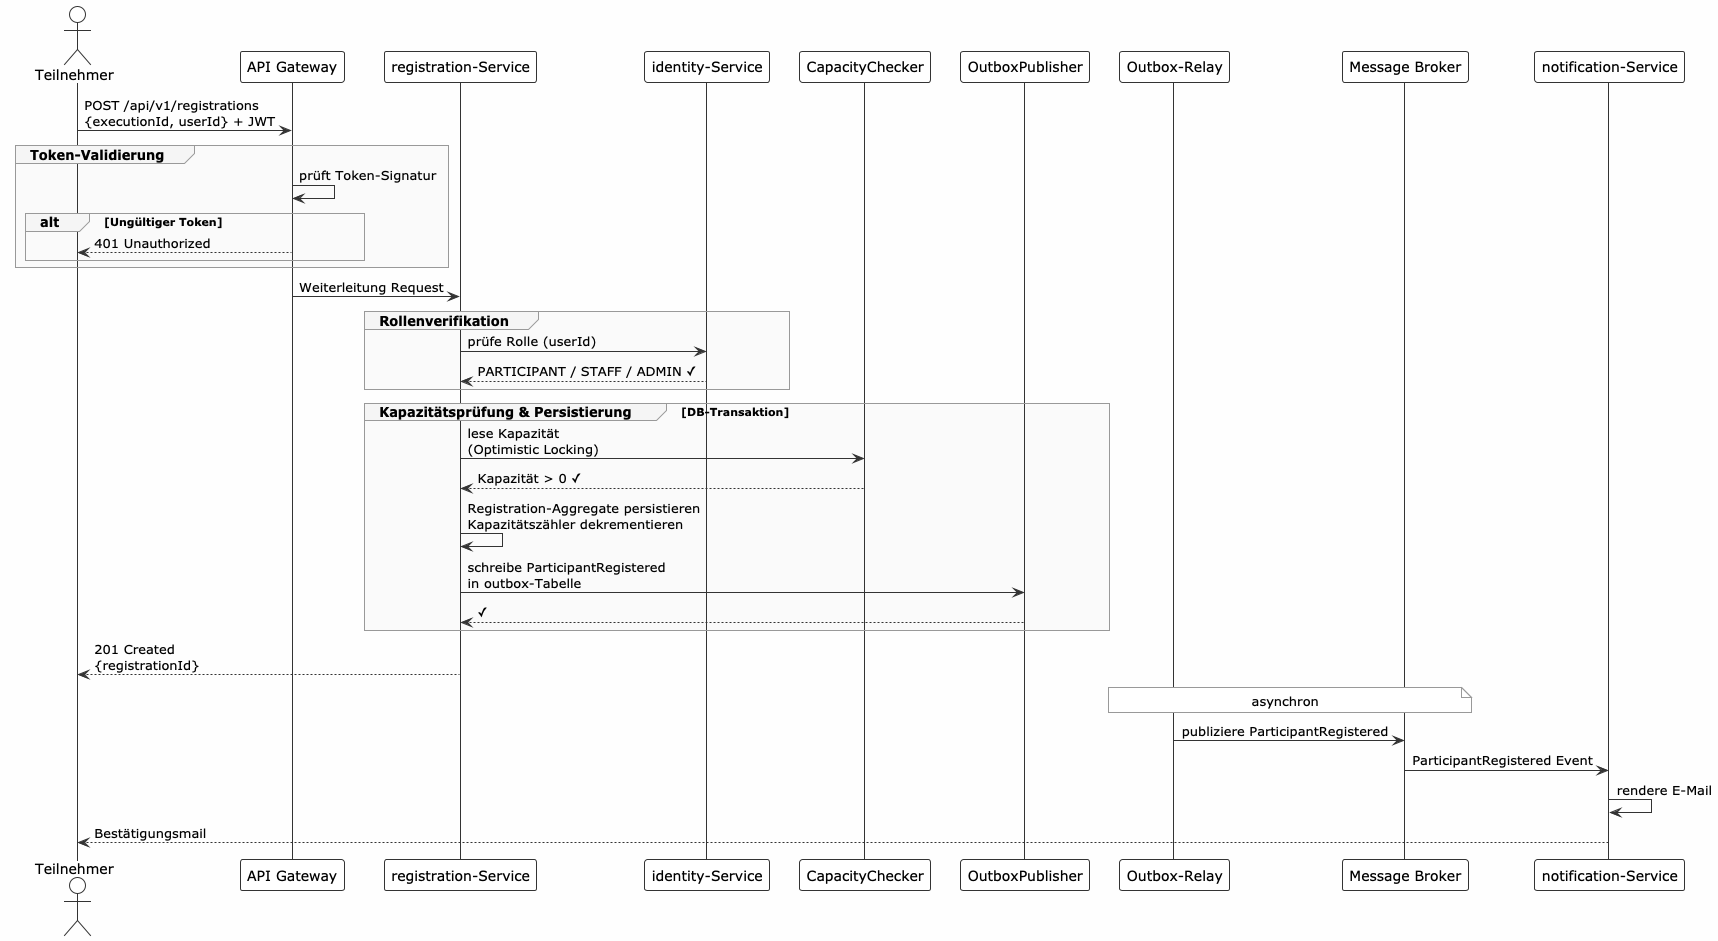
\includegraphics[width=\textwidth]{assets/sequence_diagram_1}
  \caption{\textit{Sequenz Diagramm für Teilnehmer schreibt sich ein (Happy Path)}}
  \label{fig:sequence_diagram_1}
\end{figure}


\subsection{Szenario~2: Kurs ausgebucht -- Warteliste}

Dieses Szenario behandelt den Fall, dass beim Einschreiben keine freie Kapazität mehr
vorhanden ist. Der Ablauf ist identisch mit Szenario~1 bis zur Kapazitätsprüfung;
anstelle einer Registrierung wird ein \texttt{WaitlistEntry} mit Zeitstempel und
Wartelisten-Position persistiert. Der Teilnehmer erhält eine \textbf{202~Accepted}-Antwort
sowie eine asynchrone Benachrichtigungsmail mit seiner Position.

Identisch mit Szenario~1 bis Schritt~5, dann:

\begin{enumerate}[leftmargin=2em, start=6]
  \item Kapazität = 0: WaitlistEntry mit Zeitstempel und nächster freier Position.
  \item Outbox-Event: \texttt{ParticipantAddedToWaitlist} (mit Position).
  \item Antwort: \textbf{202~Accepted} mit Wartelisten-Position.
\end{enumerate}


\begin{figure}[H]
  \centering
  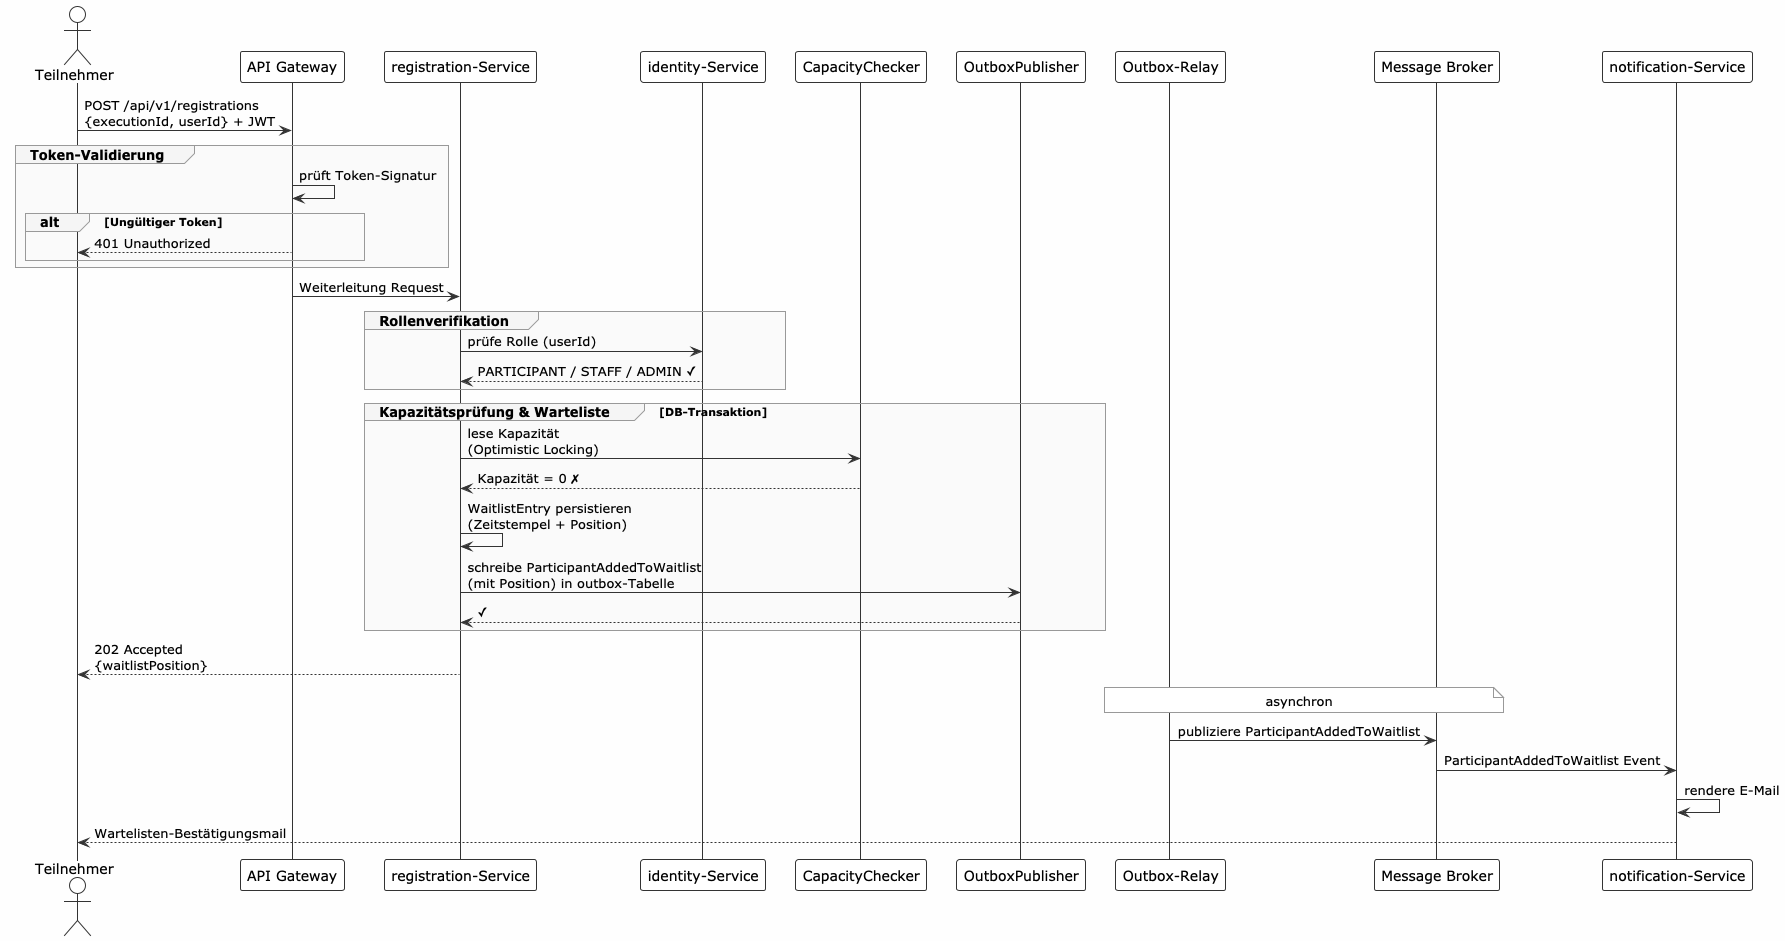
\includegraphics[width=\textwidth]{assets/sequence_diagram_2}
  \caption{\textit{Sequenz Diagramm für Teilnehmer schreibt sich ein, aber keine freien Plätze mehr }}
  \label{fig:sequence_diagram_2}
\end{figure}

\subsection{Szenario~3: Einschreibung stornieren}

Dieses Szenario beschreibt die Stornierung einer bestehenden Kursanmeldung. Nach der
Ownership-Prüfung -- nur eigene Einschreibungen dürfen storniert werden -- wird der
Status transaktional auf \texttt{CANCELLED} gesetzt und die Kapazität wieder freigegeben.
Ist die Warteliste nicht leer, rückt der älteste Eintrag automatisch nach; alle
Benachrichtigungen erfolgen asynchron über den \texttt{notification}-Service.

\begin{enumerate}[leftmargin=2em]
  \item \texttt{DELETE /api/v1/registrations/\{id\}} + JWT.
  \item Ownership-Prüfung: Nur eigene Einschreibungen dürfen storniert werden (403~Forbidden sonst).
  \item Status $\to$ CANCELLED; Kapazität inkrementiert.
  \item Outbox-Event: \texttt{RegistrationCancelled}.
  \item Falls Warteliste nicht leer: ältester Eintrag rückt nach $\to$ \texttt{WaitlistParticipantPromoted} + \texttt{ParticipantRegistered}.
  \item Antwort: \textbf{204~No~Content}.
\end{enumerate}

\begin{figure}[H]
  \centering
  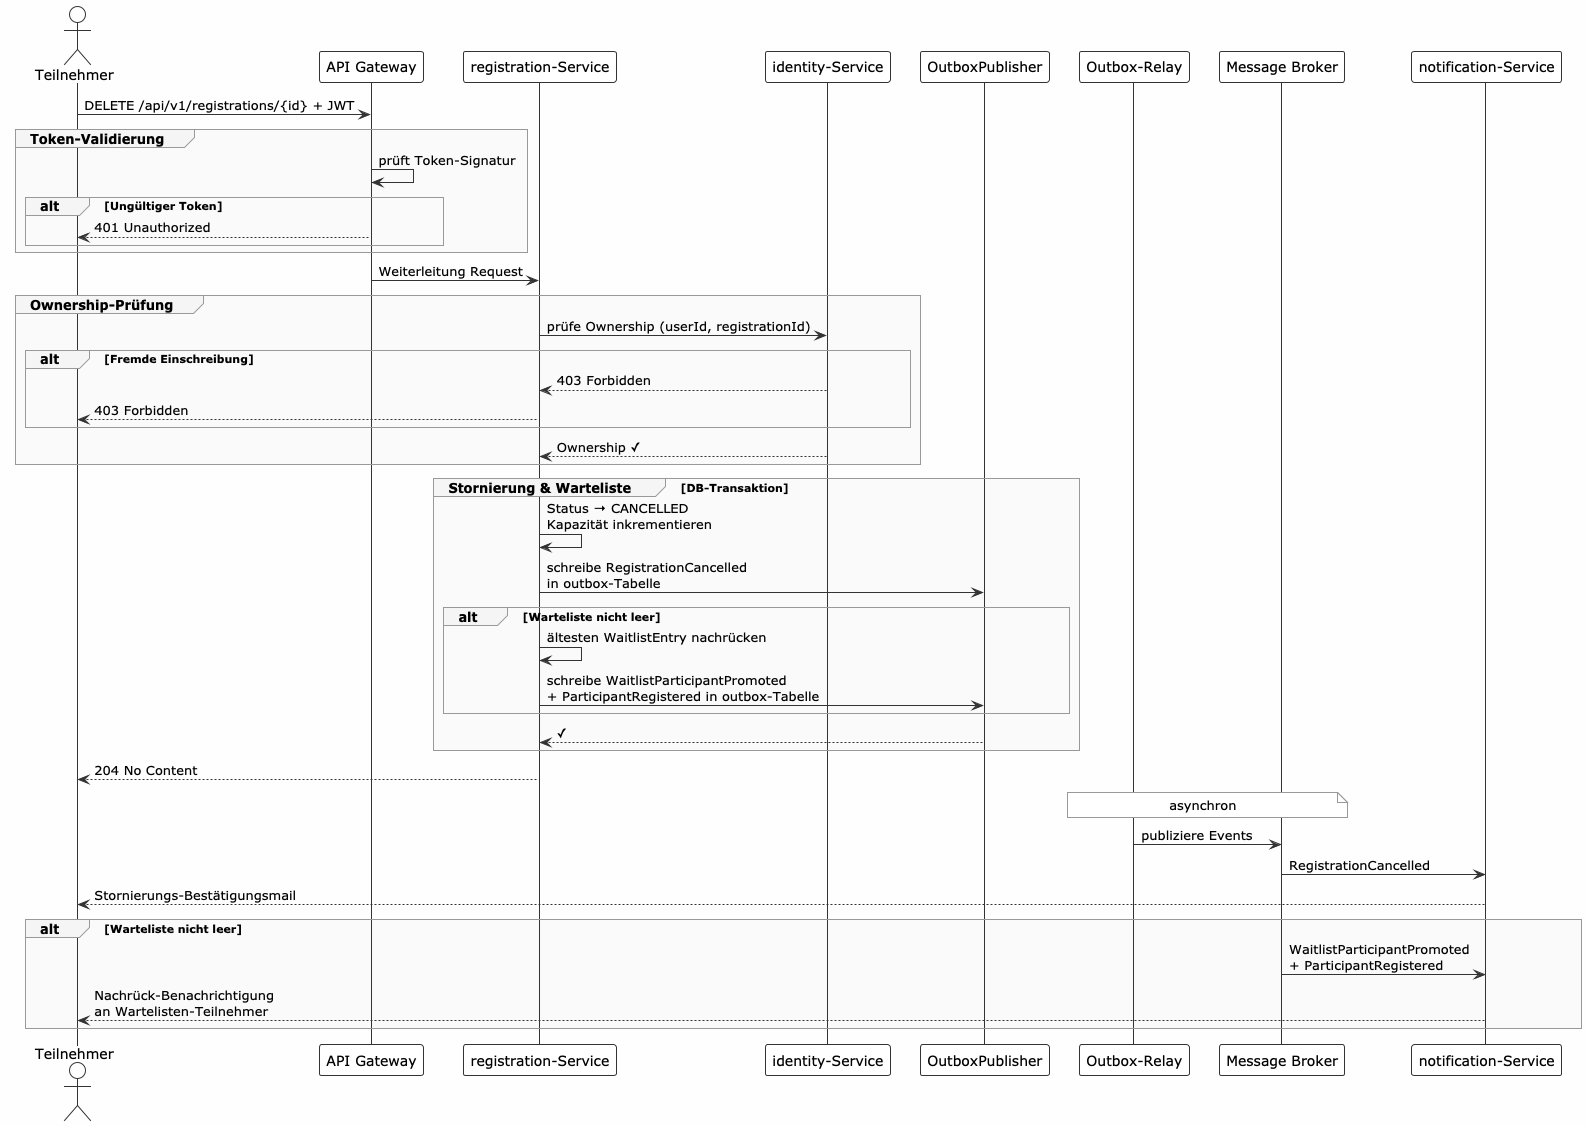
\includegraphics[width=\textwidth]{assets/sequence_diagram_3}
  \caption{\textit{Sequenz Diagramm für die Stornierung einer Kursanmeldung}}
  \label{fig:sequence_diagram_3}
\end{figure}

\subsection{Szenario~4: Admin veröffentlicht einen Kurs}

Dieses Szenario beschreibt die Veröffentlichung eines Kurses durch einen Administrator.
Der Ablauf ist bewusst schlank gehalten: Nach der Rollenprüfung -- ausschliesslich
ADMIN-Rolle ist berechtigt -- wird der \texttt{CourseStatus} transaktional von
\texttt{DRAFT} auf \texttt{PUBLISHED} gesetzt und das \texttt{CoursePublished}-Event
über die Outbox asynchron publiziert. Eine direkte Teilnehmer-Benachrichtigung
ist in diesem Szenario nicht vorgesehen.

\begin{enumerate}[leftmargin=2em]
  \item \texttt{PUT /api/v1/courses/\{id\}/publish} + JWT.
  \item ADMIN-Rolle erforderlich (403~Forbidden für alle anderen).
  \item \texttt{CourseStatus}: DRAFT $\to$ PUBLISHED.
  \item Outbox-Event: \texttt{CoursePublished}.
  \item Antwort: \textbf{200~OK}.
\end{enumerate}

\begin{figure}[H]
  \centering
  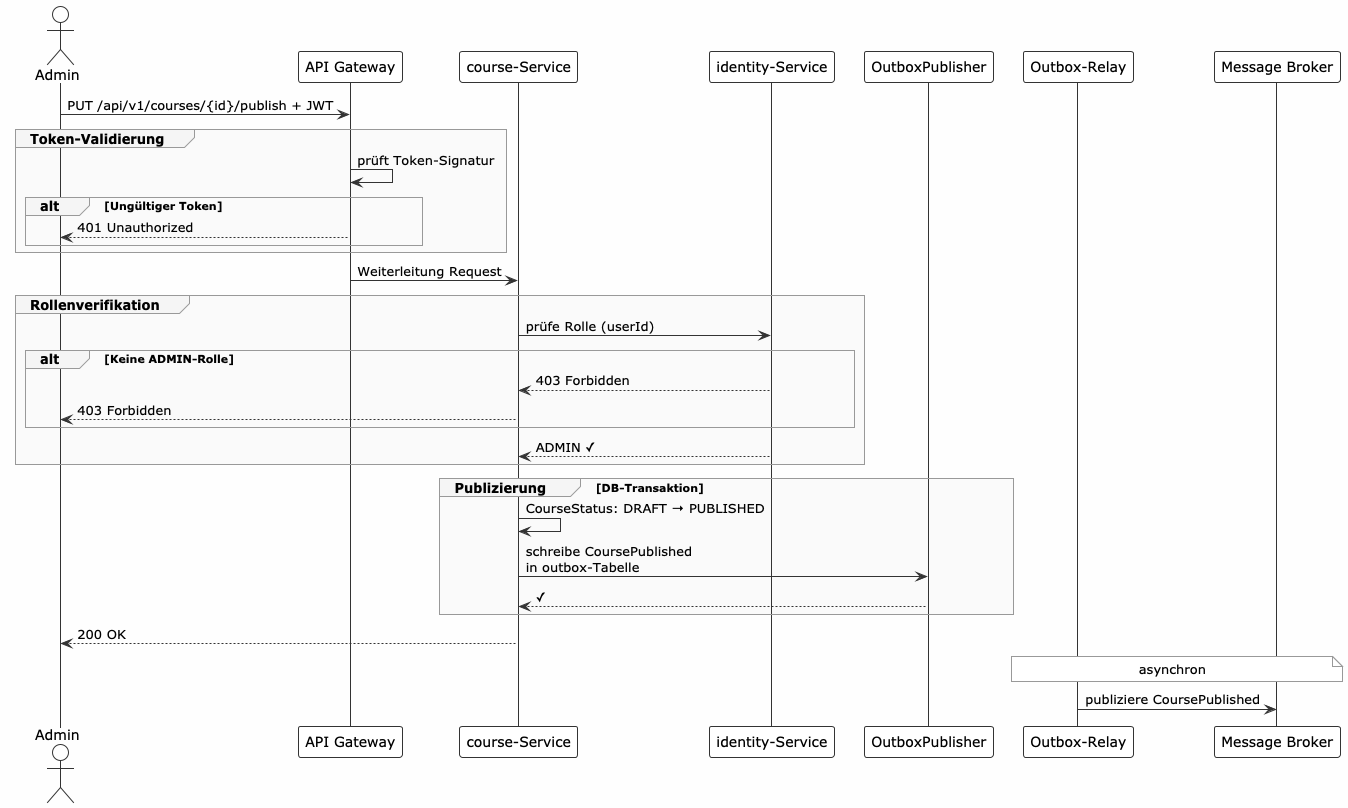
\includegraphics[width=\textwidth]{assets/sequence_diagram_4}
  \caption{\textit{Sequenz Diagramm für Admin veröffentlicht einen Kurs}}
  \label{fig:sequence_diagram_4}
\end{figure}


\subsection{Szenario~5: Cross-Context-Transaktion (Kurs archivieren)}

Dieses Szenario illustriert eine kontextübergreifende Transaktion, bei der das
Archivieren eines Kurses eine Kaskade von Zustandsänderungen in mehreren Services
auslöst. Da keine verteilte Transaktion verwendet wird, koordinieren sich
\texttt{catalog}, \texttt{scheduling}, \texttt{registration} und \texttt{notification}
ausschliesslich über Events -- die vollständige Konsistenz wird erst nach
$\sim$2--5~Sekunden erreicht (Eventual Consistency).

\begin{enumerate}[leftmargin=2em]
  \item \texttt{PUT /api/v1/courses/\{id\}/archive} (Admin).
  \item \texttt{catalog}: Status $\to$ ARCHIVED; Event \texttt{CourseArchived}.
  \item \texttt{scheduling} konsumiert $\to$ alle Executions $\to$ CANCELLED; Events \texttt{CourseExecutionCancelled}.
  \item \texttt{registration} konsumiert $\to$ alle Registrations $\to$ CANCELLED; Events \texttt{RegistrationCancelled}.
  \item \texttt{notification} versendet Massenstornierungsmails.
\end{enumerate}

\textit{Eventual Consistency:} Alle Services nach $\sim$2--5~Sek.\ konsistent.

\begin{figure}[H]
  \centering
  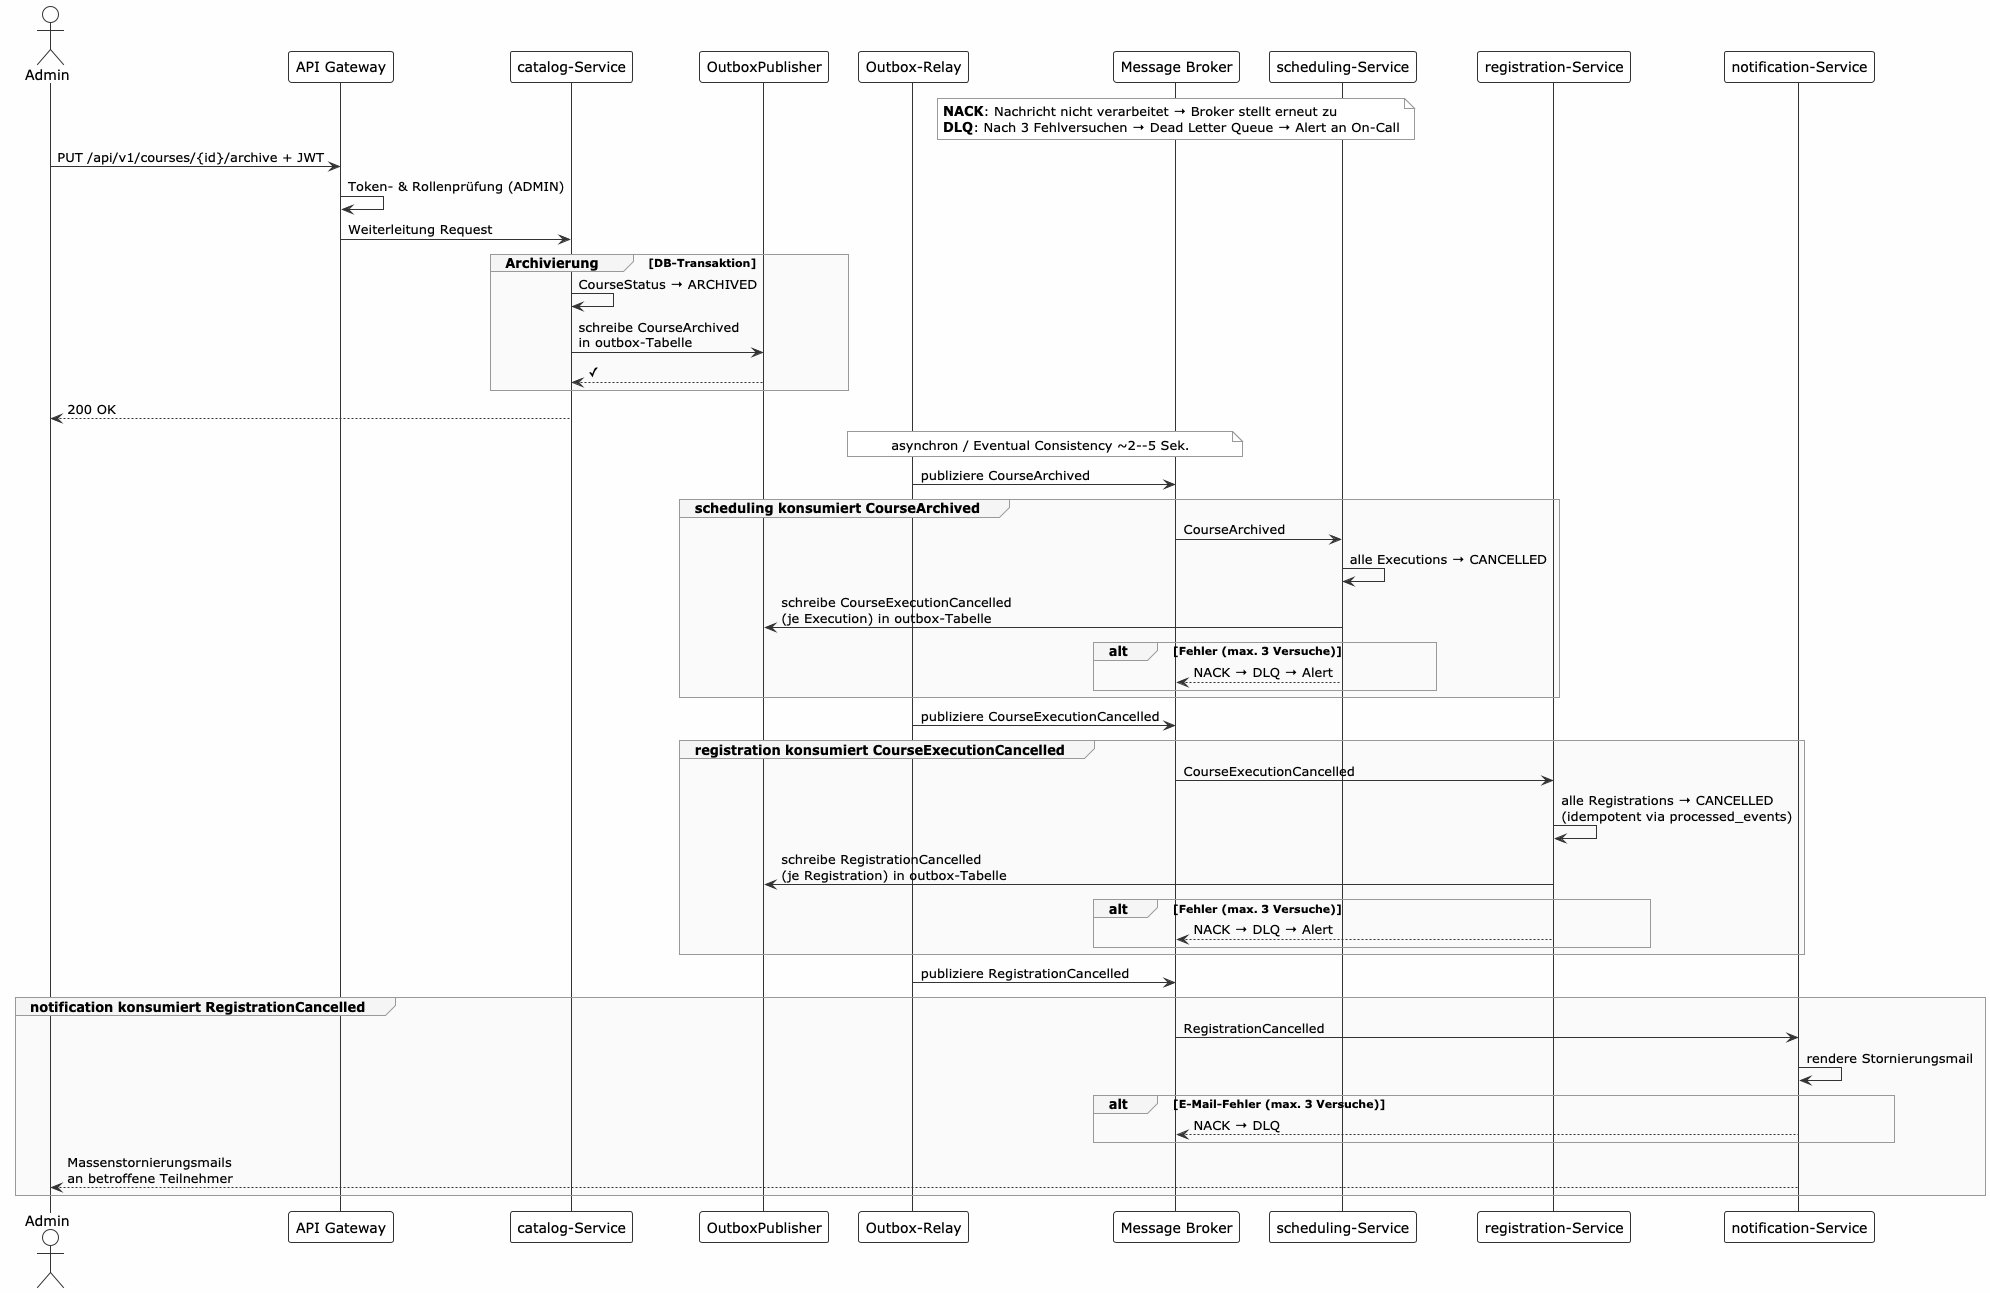
\includegraphics[width=\textwidth]{assets/sequence_diagram_5}
  \caption{\textit{Sequenz Diagramm für Kurs archivieren}}
  \label{fig:sequence_diagram_5}
\end{figure}

\begin{hinweis}[Fehlerbehandlung -- symmetrisch für alle Consumer]
  \textbf{Bei \texttt{registration}} (konsumiert \texttt{CourseExecutionCancelled}): Exception im Event-Handler $\to$
  RabbitMQ stellt erneut zu (at-least-once) $\to$ nach 3~Fehlversuchen DLQ $\to$ Alert $\to$ On-Call-Entwickler.
  Idempotenter Handler verhindert Doppelstornierungen.\\[4pt]
  \textbf{Bei \texttt{scheduling}} (konsumiert \texttt{CourseArchived}): Identischer DLQ-Mechanismus -- alle
  Executions werden auf CANCELLED gesetzt, sobald der Event erfolgreich verarbeitet ist.
  Idempotenz: \texttt{executionId} wird in \texttt{processed\_events}-Tabelle geprüft.\\[4pt]
  \textbf{Bei \texttt{notification}} (konsumiert \texttt{RegistrationCancelled}): Exception im E-Mail-Provider $\to$
  Retry (3x) $\to$ DLQ. Der Prozess (Einschreibung/Stornierung) ist bereits erfolgreich abgeschlossen.
\end{hinweis}
\newpage
\section{Verteilungssicht}

\subsection{Infrastruktur-Übersicht}

Die Produktionsumgebung läuft in der Public Cloud von Microsoft Azure mit Kubernetes
als Orchestrierungsschicht. Alle Microservices werden als containerisierte Workloads
in einem Azure Kubernetes Service (AKS) Cluster betrieben. Die Datenhaltung erfolgt
über verwaltete Azure-Dienste (Azure Database for PostgreSQL), womit Betrieb,
Patching und Backup-Management an den Cloud-Provider delegiert werden.

\begin{figure}[H]
  \centering
  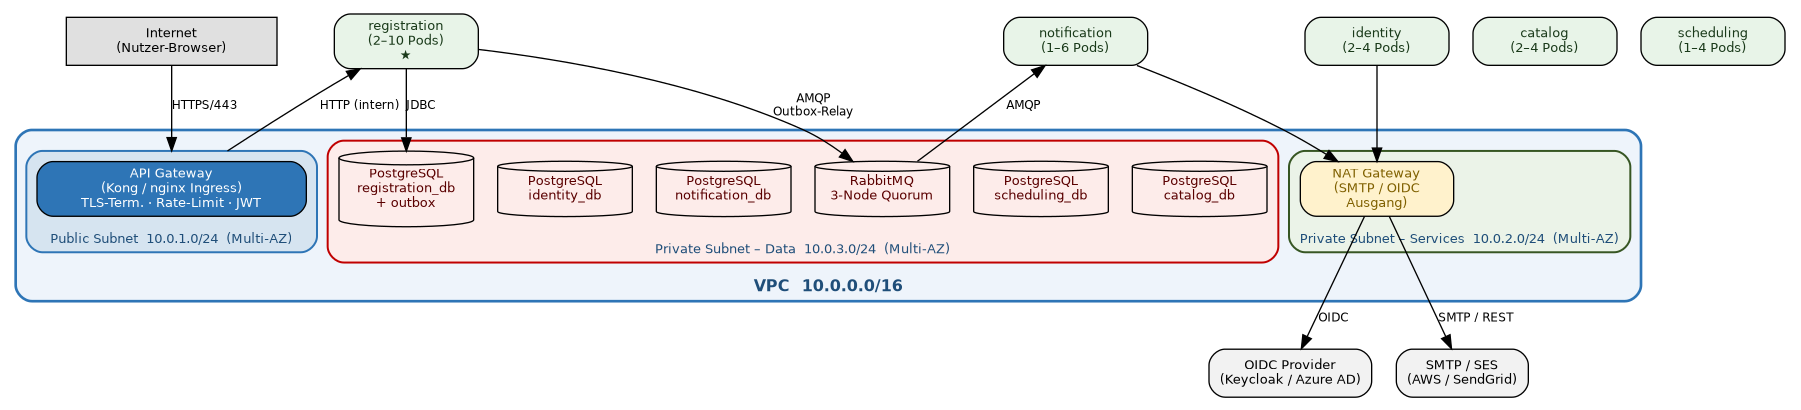
\includegraphics[width=\textwidth]{assets/deployment_diagram}
  \caption{\textit{Deployment-Diagramm: Netzwerk-Topologie (Kubernetes / Azure)}}
  \label{fig:deployment_diagram}
\end{figure}

\subsubsection{Cloud-Provider-Entscheid (ADR-010)}

Der Entscheid fiel zugunsten von \textbf{Microsoft Azure} (ADR-010). Ausschlaggebend waren:

\begin{itemize}
  \item \textbf{DSGVO-Compliance}: Azure-Regionen \textit{Switzerland North} (Zürich) und
  \textit{Switzerland West} (Genf) gewährleisten Datenresidenz in der Schweiz und
  erfüllen die Anforderungen gemäss DSG / DSGVO.
  \item \textbf{Managed Services}: Azure Database for PostgreSQL Flexible Server bietet
  automatisches Failover, PITR und integriertes Monitoring ohne Eigenaufwand.
  \item \textbf{Vendor Lock-in}: Minimiert durch den Einsatz cloud-agnostischer Technologien
  (Kubernetes, PostgreSQL, RabbitMQ) -- ein Anbieterwechsel bleibt möglich (vgl.\ R7).
  \item \textbf{Team-Kenntnisse}: Bestehendes Know-how im Betriebsteam mit Azure-Diensten
  reduziert den Einarbeitungsaufwand und das operative Risiko.
\end{itemize}

\subsection{Deployment-Umgebungen}

Das System durchläuft vier klar voneinander getrennte Umgebungen -- von der lokalen
Entwicklung bis zum produktiven Betrieb. Jede Umgebung ist auf ihren Zweck
zugeschnitten und wird über dieselbe CI/CD-Pipeline versorgt.

\begin{tabularx}{\textwidth}{L{2.5cm} L{2.5cm} X}
  \rowcolor{tableheader}
  \color{white}\textbf{Umgebung} & \color{white}\textbf{Plattform} & \color{white}\textbf{Beschreibung} \\
  Development & Docker Compose & Lokal; alle Services; vereinfachte Konfiguration (kein TLS, lokale DB). Hot-Reload. \\
  \rowcolor{tablegrey}
  Testing & K8s Namespace & Automatisch via CI/CD provisioniert; ephemeral -- nach Tests abgebaut. \\
  Staging & AKS Cluster & Produktionsähnlich; Abnahmetests; anonymisierte Prod-Daten. \\
  \rowcolor{tablegrey}
  Production & AKS Cluster (Multi-AZ) & HPA; automatische Failover-Mechanismen; Blue-Green-Deployment. \\
\end{tabularx}

\subsection{Infrastrukturkomponenten}

Die folgende Tabelle zeigt alle eingesetzten Infrastrukturkomponenten mit ihrer
konkreten Technologiewahl und Konfiguration. Die Kombination aus verwalteten
Azure-Diensten und cloud-agnostischen Open-Source-Technologien minimiert den
Betriebsaufwand bei gleichzeitig geringem Vendor Lock-in.

\begin{tabularx}{\textwidth}{L{3.2cm} L{3cm} X}
  \rowcolor{tableheader}
  \color{white}\textbf{Komponente} & \color{white}\textbf{Technologie} & \color{white}\textbf{Konfiguration} \\
  API Gateway & NGINX Ingress Controller & TLS-Terminierung, Rate-Limiting, JWT-Weiterleitung an Services;
  alternativ Spring Cloud Gateway für reaktive Routing-Logik \\
  \rowcolor{tablegrey}
  Orchestrierung & Azure Kubernetes Service~1.28+ & HPA, Readiness-/Liveness-Probes, Pod Disruption Budgets,
  Azure Monitor Integration \\
  Datenbanken & Azure Database for PostgreSQL~15 Flexible Server & Je Service eine Instanz (Database-per-Service);
  PITR~7~Tage; automatische Backups; Failover $<$~60~Sek. \\
  \rowcolor{tablegrey}
  Message Broker & RabbitMQ~3.12 & 3-Node-Quorum-Cluster; persistente Queues; DLQ; Management-UI
  über internen Ingress \\
  Monitoring & Prometheus + Grafana & RED-Pattern (Rate, Errors, Duration); Alerting bei
  Error-Rate~$>$~1\,\% und Latenz~$>$~500~ms (p99) \\
  \rowcolor{tablegrey}
  Logging & ELK-Stack & Strukturierte JSON-Logs; Correlation-ID über alle Services;
  30~Tage Retention; Index-Rotation täglich \\
  Tracing & OpenTelemetry + Jaeger & Distributed Tracing End-to-End; Sampling-Rate 10\,\%
  in Production, 100\,\% in Staging \\
  \rowcolor{tablegrey}
  CI/CD & GitHub Actions & Pipeline: Build $\to$ Unit-Tests $\to$ Integration-Tests $\to$
  Docker-Image $\to$ AKS-Deploy; automatisches Rollback bei fehlgeschlagenen Probes \\
  Secret Management & Azure Key Vault & Zentrales Secret-Management; Secrets werden zur
  Laufzeit per CSI-Treiber in Pods gemountet \\
\end{tabularx}

\subsection{Disaster Recovery Plan}

Der DR-Plan definiert verbindliche Zielwerte für Wiederherstellungszeit (RTO) und
maximal tolerierbaren Datenverlust (RPO)\footnote{RTO (Recovery Time Objective):
maximale Zeitspanne bis zur Wiederherstellung. RPO (Recovery Point Objective):
maximaler tolerierter Datenverlust in Zeit; RPO = 0~min bedeutet kein Datenverlust.}
je Infrastrukturkomponente. Die Massnahmen sind auf automatisches Failover ausgerichtet
-- manuelle Eingriffe bleiben auf Ausnahmefälle beschränkt.

\begin{tabularx}{\textwidth}{L{3cm} C{1.8cm} C{1.8cm} X}
  \rowcolor{tableheader}
  \color{white}\textbf{Komponente} & \color{white}\textbf{RTO} & \color{white}\textbf{RPO} & \color{white}\textbf{Strategie} \\
  PostgreSQL & 15~min & 5~min & Auto-Failover zu Read Replica; PITR~7~Tage; wöchentliche Restore-Tests (So, 03:00~UTC). \\
  \rowcolor{tablegrey}
  RabbitMQ & 5~min & 0~min & 3-Node Quorum-Cluster; kein Datenverlust. \\
  AKS Cluster & 30~min & N/A & Multi-AZ; Pod Disruption Budgets; Azure Availability Zones. \\
  \rowcolor{tablegrey}
  Application & 2~min & N/A & Blue-Green-Deployment; Liveness-Probes; automatisches Rollback. \\
\end{tabularx}

\begin{reviewbox}[DR-Testverantwortung]
  Der DR-Plan auf Systemebene wird halbjährlich als vollständiger Failover-Test in der Staging-Umgebung
  durchgeführt. Verantwortung: IT-Leiter (Patrick Hari). Protokoll geht an den CISO (Andrea Senn) für
  die Compliance-Dokumentation.
\end{reviewbox}

\subsection{Netzwerk-Topologie}

Das Netzwerk wird in drei Zonen aufgeteilt, die dem Prinzip der minimalen Exposition
folgen: Eingehender Verkehr läuft ausschliesslich über das öffentliche Subnet mit
NGINX Ingress; alle Microservices und Datenbankinstanzen sind in privaten Subnetzen
ohne direkten Internetzugang betrieben. Ausgehende Verbindungen der Services --
etwa für E-Mail-Versand oder OIDC -- werden über ein zentrales NAT Gateway\footnote{%
NAT Gateway (Network Address Translation): übersetzt private IP-Adressen der Services
auf eine öffentliche IP-Adresse für ausgehende Verbindungen -- ohne eingehenden
Zugriff aus dem Internet zu erlauben.} geführt.

\begin{tabularx}{\textwidth}{L{3.5cm} L{3.5cm} X}
  \rowcolor{tableheader}
  \color{white}\textbf{Netzwerkzone} & \color{white}\textbf{CIDR} & \color{white}\textbf{Beschreibung} \\
  VNet & 10.0.0.0/16 & Gesamtes Azure Virtual Network \\
  \rowcolor{tablegrey}
  Public Subnet & 10.0.1.0/24 (Multi-AZ) & NGINX Ingress / API Gateway -- einziger öffentlicher
  Zugangspunkt; Azure DDoS Protection Standard \\
  Private (Services) & 10.0.2.0/24 (Multi-AZ) & Alle Microservices -- kein direkter Internet-Zugang;
  Network Policies zwischen Services aktiv \\
  \rowcolor{tablegrey}
  Private (Data) & 10.0.3.0/24 (Multi-AZ) & PostgreSQL-Instanzen und RabbitMQ --
  nur aus Service-Subnet erreichbar; Private Endpoints \\
  NAT Gateway & Azure NAT Gateway & Ausgehende Verbindungen der Services (SMTP via
  SendGrid, OIDC-Endpunkte) \\
\end{tabularx}
\newpage
\section{Querschnittliche Konzepte}

Dieser Abschnitt beschreibt Konzepte und Entscheidungen, die nicht einem einzelnen
Service zugeordnet sind, sondern das gesamte System betreffen. Sie bilden die
gemeinsame technische Basis für Sicherheit, Betrieb, Datenhaltung und Qualitätssicherung.

\subsection{Sicherheitskonzept}

Das Sicherheitskonzept basiert auf dem Prinzip der minimalen Rechte: Authentifizierung
und Autorisierung sind konsequent voneinander getrennt, zentral über den
\texttt{identity}-Service koordiniert und in jedem Service durchgesetzt.

\subsubsection{Authentifizierung}

Die Authentifizierung ist vollständig an einen externen OIDC-Provider delegiert.
Das System selbst speichert keine Passwörter -- es vertraut ausschliesslich
signierten JWT-Tokens, deren Gültigkeit am API Gateway geprüft wird.

\begin{itemize}[leftmargin=1.5em]
  \item OIDC / OAuth~2.0: Authentifizierung vollständig extern (z.\,B.\ Keycloak, Azure~AD).
  \item JWT-Access-Token (RS256-signiert, 15~Min.), Refresh-Token (8~h).
  \item API Gateway validiert JWT-Signatur via JWKS-Endpoint; ungültig $\to$ 401.
  \item Silent Refresh: Frontend erneuert Token automatisch.
\end{itemize}

\subsubsection{Autorisierung (RBAC)}

Die Zugriffskontrolle erfolgt rollenbasiert (RBAC). Rollen werden als Claims im
JWT übertragen und von jedem Service eigenständig ausgewertet -- ein zentraler
Autorisierungs-Roundtrip entfällt damit pro Request. Der folgende
Payload-Ausschnitt zeigt die Struktur eines dekodiertes JWT:

\begin{lstlisting}
{
  "sub": "user-uuid-123",
  "roles": ["PARTICIPANT"],
  "locale": "de",
  "tenant_id": "skillbridge",
  "exp": 1700000900
}
\end{lstlisting}

E-Mail ist im OIDC-Token vorhanden, wird aber nie geloggt (PII-Schutz, Kap.~8.6).

Die folgende Tabelle zeigt, welche Aktionen den einzelnen Rollen erlaubt sind:

\begin{tabularx}{\textwidth}{X C{1.8cm} C{1.8cm} C{1.8cm} C{2.2cm}}
  \rowcolor{tableheader}
  \color{white}\textbf{Aktion} & \color{white}\textbf{Admin} & \color{white}\textbf{Staff} & \color{white}\textbf{Trainer} & \color{white}\textbf{Participant} \\
  Kurs erstellen & \yes & \yes & \no & \no \\
  \rowcolor{tablegrey}
  Kurs veröffentlichen & \yes & \no & \no & \no \\
  Kurs archivieren & \yes & \no & \no & \no \\
  \rowcolor{tablegrey}
  Durchführung planen & \yes & \yes & \no & \no \\
  Sich einschreiben & \yes & \yes & \yes & \yes \\
  \rowcolor{tablegrey}
  Eigene Stornierung & \yes & \yes & \yes & \yes \\
  Alle Einschreibungen sehen & \yes & \yes & \no & \no \\
  \rowcolor{tablegrey}
  Nutzer verwalten & \yes & \no & \no & \no \\
\end{tabularx}

\begin{hinweis}[RBAC -- Einschreiberecht für TRAINER]
  Die Berechtigung \emph{„Sich einschreiben"} für die Rolle TRAINER ist bewusst gewählt: Trainer können
  Weiterbildungsangebote ihrer Kollegen als Teilnehmer besuchen (Beispiel: ein Java-Trainer schreibt sich
  in einen Python-Kurs ein). Diese Rollenakkumulation ist im \texttt{identity}-Service durch die
  Multi-Rollen-Unterstützung abgebildet (\texttt{"roles": ["TRAINER", "PARTICIPANT"]} im JWT möglich).
  Falls ein Kursanbieter dies nicht wünscht, kann die Berechtigung per Konfiguration deaktiviert werden.
\end{hinweis}

Die folgende Tabelle beschreibt die eingesetzten Resilience-Muster, die das System
gegenüber transienten Fehlern und Kaskadenausfällen absichern:

\begin{tabularx}{\textwidth}{L{3.5cm} X}
  \rowcolor{tableheader}
  \color{white}\textbf{Muster} & \color{white}\textbf{Beschreibung} \\
  Circuit Breaker & Resilience4j: 5~Fehler in 10\,s $\to$ Open; Half-Open nach 30\,s. \\
  \rowcolor{tablegrey}
  Retry + Exp.\ Backoff & Bis zu 3×; Backoff: 100\,ms / 500\,ms / 2\,s. \\
  Dead-Letter-Queue & Nach 3~Fehlversuchen; Alerting bei DLQ-Tiefe $>$ 0. \\
  \rowcolor{tablegrey}
  Graceful Degradation & Ausfall von \texttt{notification} blockiert nie die Einschreibung. \\
  Idempotente Handler & EventId-Prüfung in \texttt{notification\_log}; Duplikate werden ignoriert. \\
  \rowcolor{tablegrey}
  Timeout & Connect-Timeout 2\,s; Read-Timeout 5\,s. \\
  Bulkhead & Separate Thread-Pools für \texttt{identity}- und \texttt{catalog}-Aufrufe. \\
\end{tabularx}



\textbf{Akzeptiertes Restrisiko: Kein mTLS in v1.0 (TS1)}

In v1.0 läuft die Service-zu-Service-Kommunikation innerhalb des
Kubernetes-Clusters über \textbf{unverschlüsseltes HTTP}.
Ein Angreifer mit Zugang zum internen Netz (z.\,B.\ durch einen
kompromittierten Pod) könnte den Datenverkehr zwischen Services mitlesen.

\textbf{Warum ist das für v1.0 tolerierbar?}
\begin{itemize}[leftmargin=1.5em]
  \item Das interne Kubernetes-Netzwerk ist durch \textbf{Network Policies}
  segmentiert: Jeder Service kommuniziert nur mit explizit erlaubten Peers.
  \item Der Perimeter ist durch TLS am API Gateway gesichert;
  kein externer Traffic erreicht die Services direkt.
  \item Das Betriebsteam hat in v1.0 kein ausreichendes Know-how für
  Sidecar-Proxies und Zertifikatsrotation (Budget- und Zeitrahmen MVP).
\end{itemize}

\textbf{Unter welchen Bedingungen muss nachgebessert werden?}
\begin{itemize}[leftmargin=1.5em]
  \item Vor Go-Live eines zweiten Tenants (Multi-Tenancy v2.0, ADR-008):
  Datentrennung auf Netzwerkebene wird dann zwingend.
  \item Bei einem Security-Audit-Befund, der dieses Muster als
  Critical/High einstuft (Kap.~1.1, Go-Live-Kriterium).
  \item Spätestens mit Einführung von v2.0:
  Linkerd ersetzt das fehlende mTLS vollständig (ADR-007, TS1).
\end{itemize}
Dieses Risiko ist als technische Schuld \textbf{TS1} erfasst und im
Tilgungsplan verankert (Kap.~11).

\subsection{Logging und Observability}

Observability ist als Querschnittsanforderung in allen Services einheitlich
umgesetzt. Strukturierte Logs, verteiltes Tracing und Prometheus-Metriken bilden
zusammen die Grundlage für Fehleranalyse, Alerting und Kapazitätsplanung im Betrieb.

\begin{tabularx}{\textwidth}{L{3cm} X}
  \rowcolor{tableheader}
  \color{white}\textbf{Aspekt} & \color{white}\textbf{Beschreibung} \\
  Strukturiertes Logging & JSON-Format (Logback + SLF4J): \texttt{timestamp, level, service, correlationId, message, exception}. \\
  \rowcolor{tablegrey}
  Correlation-ID & UUID (\texttt{X-Correlation-ID}) wird als HTTP-Header propagiert und in alle Logs geschrieben. \\
  PII-Schutz & E-Mail und Name werden vor dem Logging maskiert (Log-Scrubbing-Middleware). \\
  \rowcolor{tablegrey}
  Metriken & Prometheus (RED-Muster); exportiert via \texttt{/actuator/prometheus}. \\
  Distributed Tracing & OpenTelemetry; Traces in Jaeger; \texttt{traceparent}-Header-Propagation. \\
  \rowcolor{tablegrey}
  Alerting & Error-Rate $>$ 1\,\%, P99-Latenz $>$ 1\,s, Queue-Tiefe $>$ 500, DLQ $>$ 0, DB-Pool $>$ 90\,\%, SSL-Expiry $<$ 30~Tage. \\
\end{tabularx}

\subsection{Datenpersistenz}

Jeder Service verwaltet seine Daten vollständig autonom in einer eigenen
PostgreSQL-Instanz. Kein Service greift direkt auf die Datenbank eines anderen
zu -- Datenaustausch erfolgt ausschliesslich über Events. Dieses Muster
garantiert lose Kopplung und ermöglicht unabhängige Schema-Migrationen.

\begin{tabularx}{\textwidth}{L{3.5cm} X}
  \rowcolor{tableheader}
  \color{white}\textbf{Konzept} & \color{white}\textbf{Beschreibung} \\
  Database per Service & Eigene PostgreSQL-DB je BC; kein Cross-Service-Zugriff. \\
  \rowcolor{tablegrey}
  Optimistic Locking & \texttt{version}-Feld im Aggregate; Konflikt $\to$ 409~Conflict + Client-Retry. \\
  Transactional Outbox & Events atomar mit Domänenänderung; Relay-Prozess publiziert asynchron (vgl.\ ADR-009). \\
  \rowcolor{tablegrey}
  Schema-Migration & Flyway; versionierte SQL-Skripte; idempotent und rückwärtskompatibel. \\
  Backups & Täglich; PITR~7~Tage; wöchentliche Restore-Tests. \\
\end{tabularx}

\subsection{API-Design-Richtlinien}

Alle Services folgen denselben API-Design-Richtlinien, um eine konsistente
Schnittstelle für Clients und Service-zu-Service-Kommunikation sicherzustellen.
Grundlage ist ein \textbf{Contract-First-Ansatz} (ADR-011): Die
OpenAPI-Spezifikation (\texttt{openapi/}\allowbreak \texttt{eduplanner-}\allowbreak \texttt{api.yaml}) ist die
\emph{einzige Quelle der Wahrheit} -- Interfaces und Server-Stubs werden
daraus generiert, nicht umgekehrt.
Die vollständige Spezifikation liegt in Anhang~D.

\subsubsection{Contract-First-Workflow}

Im Contract-First-Ansatz wird die Reihenfolge gegenüber Code-First
umgekehrt: Zuerst entsteht der Vertrag, dann der Code.

\begin{enumerate}[leftmargin=2em]
  \item \textbf{Spec schreiben:} Die Datei
  \texttt{openapi/}\allowbreak \texttt{eduplanner-}\allowbreak \texttt{api.yaml} wird manuell gepflegt und
  in Git versioniert. Sie ist der einzige Ort, an dem API-Änderungen
  initiiert werden.
  \item \textbf{Stubs generieren:} Der \texttt{openapi-}\allowbreak \texttt{generator-}\allowbreak \texttt{maven-}\allowbreak \texttt{plugin}
  erzeugt beim Build automatisch Spring-Boot-Interfaces (Server-Stubs)
  aus der Spec:
\begin{lstlisting}
<!-- pom.xml (Auszug) -->
<plugin>
  <groupId>org.openapitools</groupId>
  <artifactId>openapi-generator-maven-plugin</artifactId>
  <configuration>
    <inputSpec>
      ${project.basedir}/../../openapi/eduplanner-api.yaml
    </inputSpec>
    <generatorName>spring</generatorName>
    <configOptions>
      <interfaceOnly>true</interfaceOnly>
      <useSpringBoot3>true</useSpringBoot3>
      <useTags>true</useTags>
    </configOptions>
  </configuration>
</plugin>
\end{lstlisting}
  \item \textbf{Implementieren:} Das Dev-Team implementiert die
  generierten Interfaces (\texttt{CoursesApi}, \texttt{RegistrationsApi}
  usw.). Der Compiler erzwingt Konformität -- eine Abweichung vom
  Vertrag führt zu einem Build-Fehler.
  \item \textbf{Swagger~UI bereitstellen:} Jeder Service stellt die
  interaktive Swagger~UI unter
  \texttt{/swagger-ui/index.html} bereit (via
  \texttt{springdoc-}\allowbreak \texttt{openapi-}\allowbreak \texttt{starter-}\allowbreak \texttt{webmvc-}\allowbreak \texttt{ui}).
  Die zugrundeliegende YAML-Datei ist unter
  \texttt{/v3/api-docs.yaml} abrufbar.
  \item \textbf{CI-Validierung:} Die Pipeline validiert die Spec vor
  jedem Merge mit \texttt{vacuum} (Linting) und
  \texttt{openapi-generator} (Generierbarkeit). Ein ungültiger
  Vertrag blockiert den Build.
\end{enumerate}

\begin{reviewbox}[Contract-First -- Vorteile für EduPlanner]
  \textbf{Frühe Einigung:} Frontend- und Backend-Team können parallel
  entwickeln, sobald der Vertrag feststeht -- kein Warten auf
  funktionierende Implementierungen.\\[4pt]
  \textbf{Konsistenz:} Generierte Stubs und DTOs sind immer synchron
  mit der Spec. Manuelle Abweichungen sind nicht möglich.\\[4pt]
  \textbf{Contract Testing (TS2):} Pact-Tests validieren, dass
  Consumer und Provider denselben Vertrag einhalten
  (Tilgung Sprint~8, Kap.~11.2).
\end{reviewbox}

\subsubsection{API-Design-Regeln}

\begin{itemize}[leftmargin=1.5em]
  \item \textbf{RESTful:} Ressourcenorientierte URLs, korrekte HTTP-Verben
  (GET\,/\,POST\,/\,PUT\,/\,DELETE).
  \item \textbf{Versionierung:} \texttt{/api/v1/...} --
  Breaking Changes führen zu einer neuen Major-Version
  (\texttt{/api/v2/...}). Additive Änderungen sind rückwärtskompatibel.
  \item \textbf{Swagger~UI:} Erreichbar unter
  \texttt{/swagger-ui/index.html} pro Service. Zugriffsschutz in
  Produktion via API-Gateway-Policy (nur internes Netz).
  \item \textbf{Fehlerantworten:} RFC~7807 Problem Details
  (\texttt{application/problem+json}) mit \texttt{type},
  \texttt{title}, \texttt{status}, \texttt{detail}, \texttt{instance}
  und optionalem \texttt{errors}-Array für Validierungsfehler.
  \item \textbf{Pagination:} Cursor-basiert
  (\texttt{?cursor=\ldots\&limit=20}, max.\ 100).
  Kein Offset-Paging (inkonsistent bei hoher Schreiblast).
  \item \textbf{Idempotency-Key:} Optionaler \texttt{Idempotency-Key}-Header
  (UUID) bei allen POST-Endpunkten -- verhindert Doppeleinschreibungen
  bei Netzwerkfehlern (vgl.\ Kap.~5.4).
  \item \textbf{Authentifizierung:} RS256-signierter JWT Bearer Token;
  Validierung am API Gateway; Services vertrauen dem weitergeleiteten
  Header (Defense in Depth via lokales RBAC).
\end{itemize}

\begin{hinweis}[Beispiel: RFC~7807 Fehlerantwort]
\begin{lstlisting}
{
  "type":     "https://eduplanner.skillbridge.ch/problems/validation-error",
  "title":    "Validation Error",
  "status":   400,
  "detail":   "Das Feld 'title' darf nicht leer sein.",
  "instance": "/api/v1/courses",
  "errors":   [{ "field": "title", "message": "Darf nicht leer sein." }]
}
\end{lstlisting}
\end{hinweis}

\subsection{Teststrategie (Ebene 1--3)}

Die Teststrategie folgt der Testpyramide: Schnelle, isolierte Unit-Tests bilden
die Basis; Integration- und Contract-Tests sichern das Zusammenspiel der
Komponenten; E2E- und Performance-Tests validieren das Systemverhalten unter
realistischen Bedingungen. Security- und Chaos-Tests ergänzen die Strategie
um Robustheit und Angriffssicherheit.

\begin{tabularx}{\textwidth}{L{2.2cm} L{2.5cm} X L{3.0cm}}
  \rowcolor{tableheader}
  \color{white}\textbf{Testtyp} & \color{white}\textbf{Umfang} & \color{white}\textbf{Ziel} & \color{white}\textbf{Tool / Tooling} \\
  Unit Tests & Einzelne Klassen / Aggregate & Functional Correctness; Business-Logik-Abdeckung $>$ 80\,\% & JUnit~5, Mockito. \\
  \rowcolor{tablegrey}
  Integration Tests & Slice (Controller $\to$ Repo) & Prüfung DB-Interaktion, JPA-Mappings, JSON-Serialisierung & Testcontainers (PostgreSQL). \\
  Contract Tests & Service-Schnittstellen (CDC) & API-Kompatibilität zwischen catalog/sched/reg (Tilgung TS2) & Pact (geplant ab Sprint~8). \\
  \rowcolor{tablegrey}
  E2E Tests & Krit.\ Journeys & Staging-Deploy bricht bei Fehler & Cypress; Einschreibung, Stornierung, Veröffentlichung. \\
  Performance & P95 $<$ 500\,ms & Staging-Alert bei Überschreitung & k6, 1\,000 concurrent users, wöchentlich. \\
  \rowcolor{tablegrey}
  Chaos Engineering & Wöchentlich & Ergebnisse im Wiki & Pod-Kills, Network-Delays (Chaos Mesh). \\
  Security Tests & Vor Release & Release blockiert bei Critical/High & OWASP ZAP, Trivy, Snyk. \\
\end{tabularx}
\newpage
\section{Architekturentscheidungen (ADRs)}

Architecture Decision Records (ADRs)\footnote{%
  \textit{Architecture Decision Record (ADR)}: Ein ADR ist ein kurzes, strukturiertes Dokument,
  das eine einzelne, architekturrelevante Entscheidung samt Kontext, betrachteten Alternativen
  und Begründung festhält. Das Format geht auf Michael Nygard zurück
  (\url{https://cognitect.com/blog/2011/11/15/documenting-architecture-decisions}).}
dokumentieren wichtige Architekturentscheidungen mit Kontext, Alternativen und Konsequenzen.
Jeder ADR ist unveränderlich – er wird nicht überschrieben, sondern durch einen neuen ADR
abgelöst oder ergänzt. Die nachfolgenden ADRs decken alle in diesem Dokument referenzierten
Entscheidungen vollständig ab.

% ── ADR-001 ──────────────────────────────────────────────────
\subsection{ADR-001: Microservices entlang der Bounded Contexts}

\begin{tabularx}{\textwidth}{L{3.5cm} X}
  \rowcolor{tableheader}
  \color{white}\textbf{Feld} & \color{white}\textbf{Inhalt} \\
  Status & Akzeptiert -- 2026-01-20 \\
  \rowcolor{tablegrey}
  Qualitätsziele & Maintainability (primär), Reliability-Availability, Performance Efficiency \\
  Entscheidungstreiber & Unabhängige Deploybarkeit der Teams; unterschiedliche Skalierungsbedarfe je BC; langfristige Wartbarkeit durch klare fachliche Grenzen (DDD). \\
  \rowcolor{tablegrey}
  Kontext & 5~klar abgrenzbare fachliche Domänen mit unterschiedlichen Änderungsraten, Skalierungsbedarfen und Team-Verantwortlichkeiten. \\
  Entscheidung & Jeder Bounded Context als eigenständiger Microservice mit eigenem Repository und eigener Datenbank. \\
  \rowcolor{tablegrey}
  Alternativen & (1)~\emph{Modularer Monolith} -- ernsthaft evaluiert:
  geringere Betriebskomplexität, einfachere lokale Entwicklung,
  ACID-Transaktionen über Modulgrenzen. Für ein 5--8-köpfiges Team und
  einen 6-Monats-MVP ist dies die objektiv einfachere Wahl.
  Abgelehnt wegen (a)~unterschiedlicher Skalierungsbedarfe:
  \texttt{registration} muss zur Spitzenzeit unabhängig skalieren;
  (b)~Erfahrung zeigt, dass Modulgrenzen im Monolithen mit der Zeit
  erodieren (``Big Ball of Mud''); (c)~Lernziel: Microservices
  realitätsnah dokumentieren.
  Fallback explizit geplant: falls Betriebsaufwand das Team überfordert,
  Rückbau auf modularen Monolithen (Risiko~R5).
  (2)~Zwei Services -- abgelehnt: fachliche Grenzen verwischen. \\
  Konsequenzen & (+)~Unabhängige Deployments. (+)~Team-Autonomie. (+)~Separate Skalierbarkeit. (-)~Erhöhte Betriebskomplexität. (-)~Eventual Consistency. \\
\end{tabularx}

% ── ADR-002 ──────────────────────────────────────────────────
\subsection{ADR-002: Asynchrone Kommunikation via Message Broker}

\begin{tabularx}{\textwidth}{L{3.5cm} X}
  \rowcolor{tableheader}
  \color{white}\textbf{Feld} & \color{white}\textbf{Inhalt} \\
  Status & Akzeptiert -- 2026-01-22 \\
  \rowcolor{tablegrey}
  Qualitätsziele & Reliability-Availability (primär), Maintainability, Functional Correctness \\
  Entscheidungstreiber & Resilienz bei Teilausfällen; Entkopplung von Sender und Empfänger; kein Kaskadenausfall durch synchrone Abhängigkeiten. \\
  \rowcolor{tablegrey}
  Entscheidung & Domain Events über RabbitMQ (Pub/Sub). \\
  Alternativen & (1)~Direkter REST-Aufruf -- abgelehnt: starke Kopplung, Kaskadenfehler. (2)~Polling der DB -- abgelehnt: ineffizient. (3)~Kafka -- zurückgestellt: Overkill für aktuelles Volumen. \\
  \rowcolor{tablegrey}
  Konsequenzen & (+)~Lose Kopplung. (+)~Resilienz. (-)~Eventual Consistency. (-)~Zusätzliche Infrastruktur. \\
\end{tabularx}

% ── ADR-003 ──────────────────────────────────────────────────
\subsection{ADR-003: Externer Identity Provider}

\begin{tabularx}{\textwidth}{L{3.5cm} X}
  \rowcolor{tableheader}
  \color{white}\textbf{Feld} & \color{white}\textbf{Inhalt} \\
  Status & Akzeptiert -- 2026-01-25 \\
  \rowcolor{tablegrey}
  Qualitätsziele & Security (primär), Maintainability \\
  Entscheidungstreiber & Kein eigenes Passwort-Management (Sicherheitsrisiko); MFA und SSO ohne Eigenentwicklung; DSGVO-konforme Datenhaltung beim IdP. \\
  \rowcolor{tablegrey}
  Entscheidung & Externer OIDC-konformer IdP (z.\,B.\ Keycloak). EduPlanner verwaltet keine Passwörter. \\
  Alternativen & (1)~Eigener Auth-Service -- abgelehnt: hohes Sicherheitsrisiko. (2)~Auth0/Okta -- in Evaluierung für v2.0. \\
  \rowcolor{tablegrey}
  Konsequenzen & (+)~Security-Best-Practices, MFA, SSO, DSGVO. (-)~Externe Abhängigkeit (R3). \\
\end{tabularx}

% ── ADR-004 ──────────────────────────────────────────────────
\subsection{ADR-004: Transactional Outbox für zuverlässige Events}

\begin{tabularx}{\textwidth}{L{3.5cm} X}
  \rowcolor{tableheader}
  \color{white}\textbf{Feld} & \color{white}\textbf{Inhalt} \\
  Status & Akzeptiert -- 2026-02-01 \\
  \rowcolor{tablegrey}
  Qualitätsziele & Functional Correctness (primär), Reliability-Availability \\
  Entscheidungstreiber & Atomizität zwischen DB-Schreibvorgang und Event-Publikation; Vermeidung von Dual-Write-Problem; Garantie: kein verlorenes Event. \\
  \rowcolor{tablegrey}
  Entscheidung & Events atomar mit DB-Änderung in \texttt{outbox}-Tabelle; Relay-Prozess publiziert asynchron (Technologie: ADR-009). \\
  Alternativen & (1)~Dual Write -- abgelehnt: kein Two-Phase-Commit. (2)~Event-Sourcing -- zu komplex. \\
  \rowcolor{tablegrey}
  Konsequenzen & (+)~Keine verlorenen Events. (+)~Atomare Konsistenz. (-)~Idempotente Handler erforderlich. \\
\end{tabularx}

% ── ADR-005 ──────────────────────────────────────────────────
\subsection{ADR-005: Angular SPA als Frontend-Technologie}

\begin{tabularx}{\textwidth}{L{3.5cm} X}
  \rowcolor{tableheader}
  \color{white}\textbf{Feld} & \color{white}\textbf{Inhalt} \\
  Status & Akzeptiert -- 2026-02-05 \\
  \rowcolor{tablegrey}
  Qualitätsziele & Usability (primär), Maintainability \\
  Entscheidungstreiber & Team-Kenntnisse in Vue.js und Angular vorhanden; SPA ermöglicht reaktive UX ohne Server-Round-Trip; TypeScript erhöht Wartbarkeit. \\
  \rowcolor{tablegrey}
  Entscheidung & Angular, TypeScript. \\
  Alternativen & (1)~Next.js -- zurückgestellt (v2.0). (2)~Vue.js -- als gleichwertige Alternative evaluiert; Angular gewählt aufgrund stärkerer Typisierung und integriertem Framework-Ökosystem. \\
  \rowcolor{tablegrey}
  Konsequenzen & (+)~Bekanntes Ökosystem. (+)~Starke Typisierung via TypeScript. (-)~Bundle-Grösse (Code Splitting erforderlich). (-)~SEO-Aufwand (kein SSR in v1.0). \\
\end{tabularx}

% ── ADR-006 ──────────────────────────────────────────────────
\subsection{ADR-006: PostgreSQL als primäre Datenbank}

\begin{tabularx}{\textwidth}{L{3.5cm} X}
  \rowcolor{tableheader}
  \color{white}\textbf{Feld} & \color{white}\textbf{Inhalt} \\
  Status & Akzeptiert -- 2026-02-08 \\
  \rowcolor{tablegrey}
  Qualitätsziele & Functional Correctness (primär), Reliability-Availability \\
  Entscheidungstreiber & ACID-Garantien für Transaktionen; JSONB-Support\footnote{JSONB
    (JSON Binary): speichert JSON-Daten binär dekomprimiert -- im Gegensatz zu JSON indizierbar
    (GIN-Index) und deutlich schneller abfragbar.} für flexible Payloads;
  Flyway-Kompatibilität; breite Java-Ökosystem-Unterstützung. \\
  \rowcolor{tablegrey}
  Entscheidung & PostgreSQL~15 (Managed) für alle Services. \\
  Alternativen & (1)~MySQL -- abgelehnt (JSONB-Support, Lizenz). (2)~MongoDB -- abgelehnt (ACID-Transaktionen). \\
  \rowcolor{tablegrey}
  Konsequenzen & (+)~Starke Konsistenz. (+)~JSONB-Flexibilität. (-)~Skalierbarkeit nur vertikal (Read-Replicas helfen). \\
\end{tabularx}

% ── ADR-007 ──────────────────────────────────────────────────
\subsection{ADR-007: Kein Service Mesh in v1.0}

Dieses ADR begründet den bewussten Verzicht auf ein Service Mesh (z.\,B.\ Linkerd oder Istio)
in der ersten Produktionsversion. Es korrespondiert direkt mit der technischen Schuld TS1 und
wird in v2.0 durch die Einführung von Linkerd abgelöst.

\begin{tabularx}{\textwidth}{L{3.5cm} X}
  \rowcolor{tableheader}
  \color{white}\textbf{Feld} & \color{white}\textbf{Inhalt} \\
  Status & Akzeptiert -- 2026-02-10 \\
  \rowcolor{tablegrey}
  Qualitätsziele & Maintainability (primär); Security (nachrangig) \\
  Entscheidungstreiber & Geringes Team-Know-how mit Service Mesh; erhöhter Betriebsaufwand für Sidecar-Infrastruktur übersteigt den Nutzen in v1.0; Budget- und Zeitrahmen des MVP. \\
  \rowcolor{tablegrey}
  Kontext & Ein Service Mesh ergänzt Kubernetes um mTLS\footnote{%
    \textit{mTLS (Mutual TLS):} Gegenseitige TLS-Authentifizierung, bei der sich beide Seiten
    (Client \textit{und} Server) mit einem Zertifikat ausweisen. Im Gegensatz zu einfachem TLS,
    das nur den Server authentifiziert, stellt mTLS sicher, dass auch der aufrufende Service
    vertrauenswürdig ist -- ein wichtiges Konzept zur Absicherung der Service-zu-Service-Kommunikation
    in Microservice-Architekturen.}
  zwischen Services, L7-Observability und automatisches Retry. Ohne Service Mesh kommunizieren
  Services intern über unverschlüsseltes HTTP innerhalb des privaten Kubernetes-Netzwerks. \\
  Entscheidung & Kein Service Mesh in v1.0. Netzwerk-Sicherheit wird durch Kubernetes Network Policies und TLS am API Gateway kompensiert. Tilgung: Linkerd in v2.0 (TS1). \\
  \rowcolor{tablegrey}
  Alternativen & (1)~Linkerd -- zurückgestellt auf v2.0: geringerer Overhead als Istio, bevorzugte Option. (2)~Istio -- abgelehnt: zu hohe operative Komplexität für Team-Grösse. \\
  Konsequenzen & (+)~Reduzierte Betriebskomplexität in v1.0. (+)~Schnellerer MVP-Launch. (-)~Kein mTLS intern (Sicherheitsrisiko TS1). (-)~Eingeschränkte L7-Observability. \\
\end{tabularx}

% ── ADR-008 ──────────────────────────────────────────────────
\subsection{ADR-008: Single-Tenant-Architektur in v1.0}

Dieses ADR begründet den bewussten Verzicht auf Multi-Tenancy in der ersten Version.
Es korrespondiert mit der technischen Schuld TS4 und wird in v2.0 durch ein
Schema-per-Tenant-Modell abgelöst (vgl.\ Kap.~14.3).

\begin{tabularx}{\textwidth}{L{3.5cm} X}
  \rowcolor{tableheader}
  \color{white}\textbf{Feld} & \color{white}\textbf{Inhalt} \\
  Status & Akzeptiert -- 2026-02-12 \\
  \rowcolor{tablegrey}
  Qualitätsziele & Maintainability (primär, kurzfristig); Functional Correctness \\
  Entscheidungstreiber & Zeitrahmen MVP (6 Monate); Multi-Tenancy erfordert durchgängige \texttt{tenant\_id}-Spalten, separates IdP-Realm und Tenant-Routing -- zu aufwändig für v1.0. Erste Zielgruppe: ein einzelner Kursanbieter (SkillBridge AG). \\
  \rowcolor{tablegrey}
  Kontext & Multi-Tenancy bezeichnet die Fähigkeit einer SaaS-Plattform, mehrere Mandanten (Kursanbieter) auf derselben Infrastruktur mit strikter Datentrennung zu betreiben. In v1.0 wird EduPlanner für einen einzigen Kursanbieter betrieben. \\
  Entscheidung & Single-Tenant-Betrieb in v1.0. Alle Services teilen eine gemeinsame Deployment-Instanz ohne mandantenbezogene Datentrennung. \\
  \rowcolor{tablegrey}
  Alternativen & (1)~Schema-per-Tenant von Anfang an -- abgelehnt: zu komplex für MVP-Zeitrahmen. (2)~Database-per-Tenant -- abgelehnt: zu hohe Infrastrukturkosten in v1.0. \\
  Konsequenzen & (+)~Deutlich vereinfachte Datenbankschicht in v1.0. (+)~Schnellerer MVP-Launch. (-)~Technische Schulden für v2.0 (TS4). (-)~Migration auf Multi-Tenancy erfordert Schema-Änderungen an allen Tabellen (R11). \\
\end{tabularx}

% ── ADR-009 ──────────────────────────────────────────────────
\subsection{ADR-009: Outbox Relay -- Technologiewahl}

Dieses ADR spezifiziert die konkrete Implementierung des Relay-Prozesses, der die
\texttt{outbox}-Tabelle aus ADR-004 ausliest und Events an RabbitMQ publiziert.

\begin{tabularx}{\textwidth}{L{3.5cm} X}
  \rowcolor{tableheader}
  \color{white}\textbf{Feld} & \color{white}\textbf{Inhalt} \\
  Status & Akzeptiert -- 2026-02-15 \\
  \rowcolor{tablegrey}
  Qualitätsziele & Functional Correctness (primär), Reliability-Availability \\
  Entscheidungstreiber & Einfache, wartbare Lösung ohne zusätzliche externe Abhängigkeiten; muss \textit{at-least-once}-Delivery garantieren; muss idempotent konsumierbar sein. \\
  \rowcolor{tablegrey}
  Kontext & Der Relay-Prozess ist ein Background-Thread innerhalb jedes Services, der periodisch die \texttt{outbox}-Tabelle nach \texttt{PENDING}-Einträgen abfragt, diese an RabbitMQ sendet und den Status auf \texttt{SENT} setzt. Bei Fehlern nach 5 Versuchen landet das Event in der Dead-Letter-Queue (DLQ). \\
  Entscheidung & Polling-basierter Relay-Thread (Spring \texttt{@Scheduled}, Intervall 500\,ms) innerhalb jedes Services. Kein separater Prozess, keine externe Abhängigkeit. \\
  \rowcolor{tablegrey}
  Alternativen & (1)~Debezium\footnote{\textit{Debezium}: Open-Source-Plattform für Change Data Capture (CDC), die Datenbankänderungen aus dem Transaction Log ausliest und als Events publiziert. Leistungsfähiger als Polling, aber deutlich komplexer im Betrieb.} (CDC) -- zurückgestellt auf v2.0: leistungsfähiger, aber höhere operative Komplexität. (2)~Separater Relay-Service -- abgelehnt: unnötige Infrastruktur für aktuelles Volumen. \\
  Konsequenzen & (+)~Keine zusätzliche Infrastruktur. (+)~Einfach zu debuggen. (-)~Polling-Latenz ($\leq$\,500\,ms). (-)~Erhöhte DB-Last bei hohem Event-Volumen. \\
\end{tabularx}

% ── ADR-010 ──────────────────────────────────────────────────
\subsection{ADR-010: Cloud-Provider -- Microsoft Azure}

Dieses ADR dokumentiert die Wahl von Microsoft Azure als Cloud-Provider für alle
Produktions- und Staging-Umgebungen von EduPlanner (vgl.\ Kap.~7.1.1).

\begin{tabularx}{\textwidth}{L{3.5cm} X}
  \rowcolor{tableheader}
  \color{white}\textbf{Feld} & \color{white}\textbf{Inhalt} \\
  Status & Akzeptiert -- 2026-02-20 \\
  \rowcolor{tablegrey}
  Qualitätsziele & Reliability-Availability (primär), Security, Maintainability \\
  Entscheidungstreiber & DSGVO/DSG-Compliance mit Datenresidenz Schweiz; Managed Services für PostgreSQL und Kubernetes; bestehendes Team-Know-how mit Azure; Budget $\leq$ CHF~800/Monat. \\
  \rowcolor{tablegrey}
  Kontext & EduPlanner muss personenbezogene Daten ausschliesslich in der EU bzw.\ der Schweiz speichern (Kap.~2.3). Nicht alle Cloud-Provider bieten Schweizer Regionen mit vollständigem Managed-Service-Angebot an. \\
  Entscheidung & Microsoft Azure mit primärer Region \textit{Switzerland North} (Zürich) und Failover-Region \textit{Switzerland West} (Genf). Eingesetzte Managed Services: Azure Kubernetes Service (AKS~1.28+), Azure Database for PostgreSQL~15 Flexible Server, Azure Key Vault, Azure Monitor. \\
  \rowcolor{tablegrey}
  Alternativen & (1)~AWS -- abgelehnt: Schweizer Region (\textit{eu-central-2}) verfügbar, aber geringeres Team-Know-how; höhere Migrationskosten. (2)~Google Cloud -- abgelehnt: kein Schweizer Rechenzentrum zum Entscheidungszeitpunkt. (3)~On-Premise -- ausgeschlossen durch Randbedingung (Kap.~2.1). \\
  Konsequenzen & (+)~Datenresidenz Schweiz erfüllt DSGVO/DSG. (+)~Managed PostgreSQL: automatisches Failover, PITR, integriertes Monitoring. (+)~Team-Know-how reduziert Einarbeitungsaufwand. (-)~Gewisser Vendor Lock-in (mitigiert durch cloud-agnostische Tools: K8s, PostgreSQL, RabbitMQ -- vgl.\ R7). \\
\end{tabularx}

% ── ADR-011 ──────────────────────────────────────────────────
\subsection{ADR-011: Contract-First mit OpenAPI~3.1 und Swagger~UI}

Dieses ADR begründet den Contract-First-Ansatz mit OpenAPI~3.1.0 als
verbindliche Entwicklungsstrategie für alle REST-Schnittstellen von
EduPlanner sowie die Bereitstellung der interaktiven Swagger~UI pro Service.
Die konsolidierte Spezifikation liegt in Anhang~D.

\begin{tabularx}{\textwidth}{L{3.5cm} X}
  \rowcolor{tableheader}
  \color{white}\textbf{Feld} & \color{white}\textbf{Inhalt} \\
  Status & Akzeptiert -- 2026-02-22 \\
  \rowcolor{tablegrey}
  Qualitätsziele & Maintainability (primär), Functional Correctness, Usability \\
  Entscheidungstreiber &
  API-First als verbindliche Randbedingung (Kap.~2.1);
  vollständige OpenAPI-Dokumentation als Go-Live-Kriterium v1.0 (Kap.~1.1);
  Contract Testing (TS2) setzt maschinenlesbare Spec voraus;
  parallele Frontend-/Backend-Entwicklung ohne Warten auf Implementierung. \\
  \rowcolor{tablegrey}
  Kontext &
  Im \emph{Code-First}-Ansatz (z.\,B.\ Springdoc-Annotationen) entsteht
  die Spec nachgelagert aus dem Code -- sie beschreibt, was implementiert
  wurde, nicht was vereinbart wurde. Dies führt zu Drift zwischen Spec
  und Implementierung sowie zu blockierter Frontend-Entwicklung.
  Im \emph{Contract-First}-Ansatz ist die YAML-Datei die einzige
  Quelle der Wahrheit: Sie entsteht zuerst, wird in Git versioniert,
  und Server-Stubs werden daraus generiert. Der Compiler erzwingt
  Konformität. \\
  Entscheidung &
  \textbf{Contract-First} mit OpenAPI~3.1.0 (YAML).
  Die Datei \texttt{openapi/}\allowbreak \texttt{eduplanner-}\allowbreak \texttt{api.yaml} wird manuell gepflegt.
  Server-Stubs (Spring-Boot-Interfaces) werden via
  \texttt{openapi-generator-}\allowbreak\texttt{maven-plugin} generiert
  (\texttt{interfaceOnly=true},\newline\texttt{useSpringBoot3=true}).
  Das Dev-Team implementiert ausschliesslich die generierten Interfaces.
  Jeder Service stellt die interaktive Swagger~UI unter
  \texttt{/swagger-ui/}\allowbreak\texttt{index.html} bereit
  (\texttt{springdoc-openapi-}\allowbreak\texttt{starter-webmvc-ui});
  in Produktion nur aus dem internen Netz erreichbar.
  Die Spec wird in der CI-Pipeline mit \texttt{vacuum} (Linting) und
  \texttt{openapi-generator} (Generierbarkeit) validiert --
  ein ungültiger Vertrag blockiert den Build. \\
  \rowcolor{tablegrey}
  Alternativen &
  (1)~\emph{Code-First / Springdoc:} abgelehnt -- Spec entsteht
  nachgelagert, Frontend-Entwicklung blockiert, Drift möglich.
  (2)~\emph{GraphQL:} zurückgestellt auf v2.0 als optionale Schicht
  neben REST (Kap.~14.3).
  (3)~\emph{AsyncAPI:} evaluiert für Domain Events (RabbitMQ);
  zurückgestellt auf v1.1 -- ergänzt OpenAPI, ersetzt es nicht.
  (4)~\emph{Keine formale Spec:} abgelehnt -- Contract Testing (TS2)
  und externes Onboarding nicht möglich. \\
  Konsequenzen &
  (+)~Spec und Implementierung sind strukturell nie aus dem Sync
  (Compiler-Enforcement). \newline
  (+)~Frontend kann mit generierten TypeScript-Clients parallel
  entwickeln. \newline
  (+)~Swagger~UI (\texttt{/swagger-ui/index.html}) bietet
  interaktives API-Testing ohne externes Tool. \newline
  (+)~Basis für Pact Contract Tests (TS2-Tilgung Sprint~8). \newline
  (-)~Initiale Spec-Erstellung erfordert Disziplin; kein ``quick
  and dirty'' Endpoint möglich. \newline
  (-)~OpenAPI beschreibt nur synchrone REST -- für asynchrone
  Domain Events ist AsyncAPI ergänzend nötig (v1.1). \\
\end{tabularx}

\newpage
\section{Qualitätsanforderungen}

Dieses Kapitel beschreibt die nichtfunktionalen Anforderungen an EduPlanner anhand von ISO/IEC~25010 Qualitätskategorien. Die Anforderungen werden zunächst als hierarchischer Qualitätsbaum strukturiert und anschließend in messbaren Szenarien konkretisiert, die als Grundlage für Architekturentscheidungen und Akzeptanztests dienen.

\subsection{Qualitätsbaum}

Der Qualitätsbaum (arc42~v9: Pflicht) gibt eine hierarchische Übersicht aller relevanten Qualitätseigenschaften von EduPlanner, gegliedert nach ISO/IEC~25010 Hauptkategorien. Er dient als Navigation in die konkreten Szenarien in Kap.~10.2 und ermöglicht die schnelle Priorisierung im ATAM-light-Prozess.

\begin{figure}[H]
  \centering
  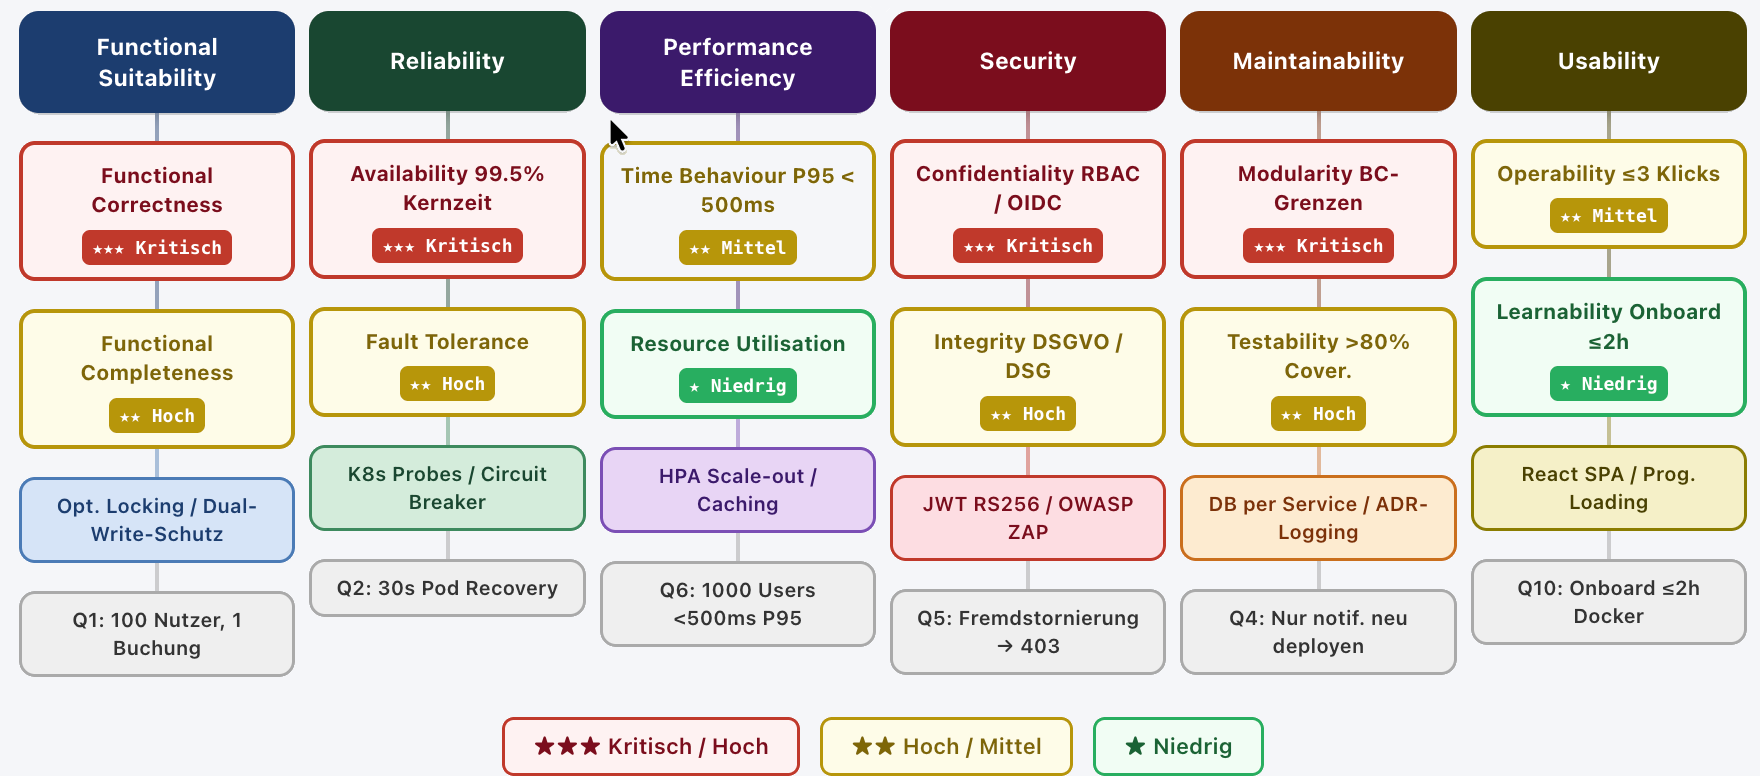
\includegraphics[width=\textwidth]{assets/QualityTree}
  \caption{\textit{Qualitätsbaum: EduPlanner Qualitätsanforderungen}}
  \label{fig:QualityTree}
\end{figure}

\textbf{ATAM-light -- Wesentliche Trade-offs in EduPlanner:}\footnote{%
  \textit{Architecture Tradeoff Analysis Method (ATAM):} Strukturierte Methode zur Architekturbewertung,
  die konkurrierende Qualitätsziele systematisch analysiert und Trade-offs explizit macht.
  „ATAM-light" bezeichnet hier eine vereinfachte, projektangepasste Variante ohne vollständigen ATAM-Workshop.}

\begin{description}[leftmargin=0pt, style=nextline]

  \item[Microservices (ADR-001):
    $\uparrow$~Maintainability,\;$\uparrow$~Scalability,\;$\downarrow$~Betriebskomplexität]
  Jeder Bounded Context wird als eigenständiger Service deployt.
  \textit{Gewinn:} Ein Team kann den \texttt{registration}-Service ändern und deployen,
  ohne dass andere Services neu gestartet werden müssen -- das erhöht die
  Wartbarkeit erheblich. Ausserdem kann der \texttt{registration}-Service zur
  Einschreibungsfrist auf 10~Pods hochskaliert werden, während
  \texttt{catalog} bei 1~Pod bleibt.
  \textit{Preis:} Das System besteht nun aus fünf laufenden Prozessen, fünf
  Datenbanken, einem Message Broker und einem API Gateway -- all das muss
  überwacht, gepatcht und betrieben werden. Ein Entwickler, der lokal arbeitet,
  startet nicht mehr eine Applikation, sondern eine ganze Landschaft via Docker
  Compose. Dieser Overhead ist das bewusst eingegangene Risiko für die
  gewonnene Unabhängigkeit (vgl.\ Risiko R5).

  \item[Asynchrones Messaging (ADR-002):
    $\uparrow$~Availability,\;$\uparrow$~Maintainability,\;$\downarrow$~Eventual Consistency]
  Zustandsändernde Ereignisse zwischen Services (z.\,B.\ ``Teilnehmer eingeschrieben'')
  werden nicht per direktem REST-Aufruf übermittelt, sondern als Domain Event über
  RabbitMQ publiziert.
  \textit{Gewinn:} Fällt der \texttt{notification}-Service aus, scheitert
  deshalb \emph{nicht} die Einschreibung -- das Event wartet in der Queue,
  bis der Service wieder läuft. Die Services sind entkoppelt und können
  unabhängig voneinander geändert werden.
  \textit{Preis:} Das System ist nicht sofort konsistent. Nach dem Archivieren
  eines Kurses sind die abhängigen Durchführungen und Einschreibungen erst nach
  ca.\ 2--5~Sekunden ebenfalls auf ``storniert'' gesetzt. Ein Admin, der
  unmittelbar nach dem Archivieren nachschaut, könnte kurzzeitig noch offene
  Einschreibungen sehen. Dieses Verhalten (Eventual Consistency) muss im
  Frontend und in der Dokumentation explizit kommuniziert werden.

  \item[Single-Tenant v1.0 (ADR-008):
    $\uparrow$~Maintainability kurzfristig,\;$\downarrow$~Technische Schulden v2.0]
  In v1.0 wird EduPlanner für \emph{einen einzigen} Kursanbieter betrieben.
  Jede Datenbanktabelle enthält keine \texttt{tenant\_id}-Spalte; das Routing
  auf verschiedene Mandanten entfällt.
  \textit{Gewinn:} Die Datenbankschicht ist erheblich einfacher -- keine
  mandantenbezogenen Abfragen, kein Tenant-Routing, kein separates
  IdP-Realm pro Kursanbieter. Das beschleunigt den MVP deutlich.
  \textit{Preis:} Sobald in v2.0 mehrere Kursanbieter auf derselben
  Infrastruktur betrieben werden sollen (echtes SaaS), muss \emph{jede}
  Tabelle um eine \texttt{tenant\_id}-Spalte ergänzt werden. Das ist eine
  aufwändige, riskante Datenmigration an allen Services gleichzeitig
  (Risiko R11, Tilgung TS4).

  \item[Kein Service Mesh in v1.0 (ADR-007):
    $\uparrow$~Betriebseinfachheit,\;$\downarrow$~Security (kein mTLS intern)]
  Ein Service Mesh (z.\,B.\ Linkerd) würde automatisch verschlüsselte
  Verbindungen zwischen allen Services herstellen (mTLS: gegenseitige
  TLS-Authentifizierung) sowie L7-Observability und automatische Retries liefern.
  \textit{Gewinn des Verzichts:} Das Team muss sich in v1.0 nicht mit
  Sidecar-Proxies, Zertifikatsrotation und Mesh-Konfiguration befassen.
  Der Betriebsaufwand bleibt im Rahmen des Budgets und der Teamgrösse.
  \textit{Preis:} Die Service-zu-Service-Kommunikation innerhalb des
  Kubernetes-Clusters läuft über unverschlüsseltes HTTP. Ein Angreifer,
  der Zugang zum internen Netz erlangt (z.\,B.\ durch einen kompromittierten
  Pod), könnte den Datenverkehr mitlesen. Dieses Risiko wird durch
  Kubernetes Network Policies mitigiert, ist aber als technische Schuld
  TS1 explizit erfasst und wird in v2.0 durch Linkerd geschlossen.

\end{description}

\subsection{Qualitätsszenarien}

Die nachfolgende Tabelle konkretisiert die im Qualitätsbaum identifizierten
Eigenschaften als messbare Szenarien nach dem arc42-Schema.

\begin{hinweis}[Methodischer Aufbau der Szenarien]
  Jedes Szenario folgt drei klar getrennten Schritten:
  \begin{enumerate}[leftmargin=2em, topsep=2pt]
  \item \textbf{Stimulus:} Was passiert -- die auslösende Situation oder
  der Auslöser (Nutzeraktion, Systemereignis, Fehler).
  \item \textbf{Erwartete Reaktion:} Was das System daraufhin tun muss --
  das architektonisch verankerte Verhalten.
  \item \textbf{Nachweis (Spalte ``Messbar''):} Wie die Erfüllung
  objektiv überprüft wird -- Testwerkzeug, Logdatei,
  Audit-Report o.\,ä. Erst durch den Nachweis wird ein Szenario
  im Architekturreview belastbar.
  \end{enumerate}
  Die Szenarien bilden die Akzeptanzkriterien für Architekturreviews
  und sind die Basis für Lasttests (Kap.~8.5) und den Security-Audit
  (Go-Live-Kriterium v1.0, Kap.~1.1).
\end{hinweis}

% Paket in der Präambel: \usepackage{xltabular}
\begin{xltabular}{\textwidth}{@{}
    >{\centering\arraybackslash}p{0.7cm}   % #
    >{\raggedright\arraybackslash}p{2.2cm}  % Attribut
  X                                        % Stimulus  (dehnt sich)
  X                                        % Erwartete Reaktion (dehnt sich)
    >{\raggedright\arraybackslash}p{3.2cm}  % Messbar
  @{}}
  \rowcolor{tableheader}
  \color{white}\textbf{\#} &
  \color{white}\textbf{Attribut} &
  \color{white}\textbf{Stimulus} &
  \color{white}\textbf{Erwartete Reaktion} &
  \color{white}\textbf{Messbar} \\
  \endfirsthead

  \rowcolor{tableheader}
  \color{white}\textbf{\#} &
  \color{white}\textbf{Attribut} &
  \color{white}\textbf{Stimulus} &
  \color{white}\textbf{Erwartete Reaktion} &
  \color{white}\textbf{Messbar} \\
  \endhead

  Q1 & Functional Correctness &
  100 Nutzer buchen letzten Platz gleichzeitig &
  Genau 1 Einschreibung; 99 Wartelisteneinträge; keine Überbuchung &
  k6\footnote{%
    \textit{k6} ist ein Open-Source-Lasttest-Tool (Grafana Labs), mit dem HTTP-Szenarien
    in JavaScript definiert und automatisiert gegen APIs ausgeführt werden.
    „Assertions" prüfen dabei automatisch die Korrektheit der Antworten.}
  Lasttest mit Assertions (ADR-004) \\

  \rowcolor{tablegrey}
  Q2 & Reliability -- Avail. &
  Pod-Neustart von \texttt{registration} &
  System reagiert in 30\,s; 2.\ Instanz übernimmt &
  K8s-Probe-Logs (ADR-001) \\

  Q3 & Reliability -- Avail. &
  \texttt{notification} fällt aus &
  Einschreibungen möglich; E-Mails nach Recovery ($\leq$ 10\,min) &
  Chaos~Engineering (ADR-002) \\

  \rowcolor{tablegrey}
  Q4 & Maintainability &
  Neues E-Mail-Template hinzufügen &
  Nur \texttt{notification}-Deploy; kein Re-Deploy anderer Services &
  Deploy-Log (ADR-001) \\

  Q5 & Security &
  Fremdstornierung durch Teilnehmer &
  403~Forbidden; Audit-Log; keine Datenänderung &
  Penetrationstest (Kap.~8.1) \\

  \rowcolor{tablegrey}
  Q6 & Performance Eff. &
  1\,000 concurrent Nutzer, Kurskatalog &
  P95 $<$ 500\,ms; Error-Rate $<$ 0,1\,\% &
  k6 Lasttest \\

  Q7 & Security &
  Abgelaufenes JWT &
  401 in $<$ 100\,ms; kein Datenzugriff &
  Automat.\ Test (Kap.~8.1.1) \\

  \rowcolor{tablegrey}
  Q8 & Privacy / Security &
  Nutzer beantragt Löschung &
  PII\footnote{%
    \textit{Personally Identifiable Information (PII):} Alle Daten, die eine natürliche Person
    direkt oder indirekt identifizierbar machen, z.\,B.\ Name, E-Mail-Adresse oder IP-Adresse
    (vgl.\ Art.~4 Nr.~1 DSGVO).}
  in 30~Tagen gelöscht/anonymisiert &
  Manueller Akzeptanztest (Kap.~8.6) \\

  Q9 & Functional Corr. &
  Stornierung + gleichzeitiges Nachrücken &
  Genau 1~Nachrücker; keine Doppelbuchung &
  Concurrency-Test (Kap.~6.6) \\

  \rowcolor{tablegrey}
  Q10 & Maintainability &
  Neuer Entwickler ongeboardet &
  Docker Compose lauffähig in $\leq$ 2\,h &
  Onboarding-Checkliste \\

  Q11 & Performance Eff. &
  10\,000 Einschreibungen/Stunde\footnote{%
    Dieser Wert modelliert ein Spitzenlastszenario, wie es z.\,B.\ zum Semesterstart auftreten kann,
    wenn viele Studierende gleichzeitig Kurse buchen. Er entspricht ca.\ 2{,}8 Einschreibungen pro Sekunde
    und ist damit als realistisches Worst-Case-Szenario für EduPlanner zu verstehen.} &
  P95 $<$ 1\,s; HPA skaliert auf max.\ 10~Pods &
  k6 in Staging (Kap.~4.6) \\

  \rowcolor{tablegrey}
  Q12 & Compliance &
  DSGVO-Audit &
  Controls dokumentiert; Löschkonzept nachgewiesen &
  Audit-Report (Kap.~8.6) \\

  Q13 & Maintainability &
  6.\ Service ``payment'' hinzufügen &
  Kein Refactoring bestehender Services; $\leq$ 2~Sprints &
  Architecture Review (ADR-001) \\

  \rowcolor{tablegrey}
  Q14 & Maintainability &
  \texttt{registration} isoliert testen &
  Unit Tests ohne Netzwerk/DB; Integration Tests $<$ 5\,min &
  CI-Laufzeit (Kap.~8.5) \\

  Q15 & Maintainability &
  Neuer externer API-Konsument onboarded &
  Swagger~UI unter \texttt{/swagger-ui/index.html} erreichbar; Server-Stub aus Spec generierbar; Client-Stub in $\leq$ 30~min &
  Contract-First CI-Validierung; \texttt{openapi-generator} (ADR-011, Anhang~D) \\

\end{xltabular}


\newpage
\section{Risiken und technische Schulden}

Dieses Kapitel dokumentiert die identifizierten Architektur- und Projektrisiken sowie die bewusst eingegangenen technischen Schulden von EduPlanner. Ziel ist es, Risiken frühzeitig sichtbar zu machen, ihre Eintrittswahrscheinlichkeit und ihren potenziellen Schaden zu bewerten und konkrete Gegenmassnahmen festzuhalten. Technische Schulden werden priorisiert und mit einem Tilgungsplan versehen, um einen kontrollierten Abbau im Projektverlauf sicherzustellen.

\subsection{Identifizierte Risiken}

Die nachfolgende Tabelle erfasst alle bekannten Risiken und bewertet sie anhand zweier Dimensionen: Wahrscheinlichkeit~(W) und Impact~(I), jeweils auf einer vierstufigen Skala (Niedrig~/ Mittel~/ Hoch~/ Kritisch). Zu jedem Risiko ist eine konkrete Gegenmassnahme definiert. Die Risikobewertungsmatrix in Abb.~\ref{fig:RiskMatrix} visualisiert die Verteilung aller Risiken und macht kritische Cluster auf einen Blick erkennbar.

\begin{figure}[H]
  \centering
  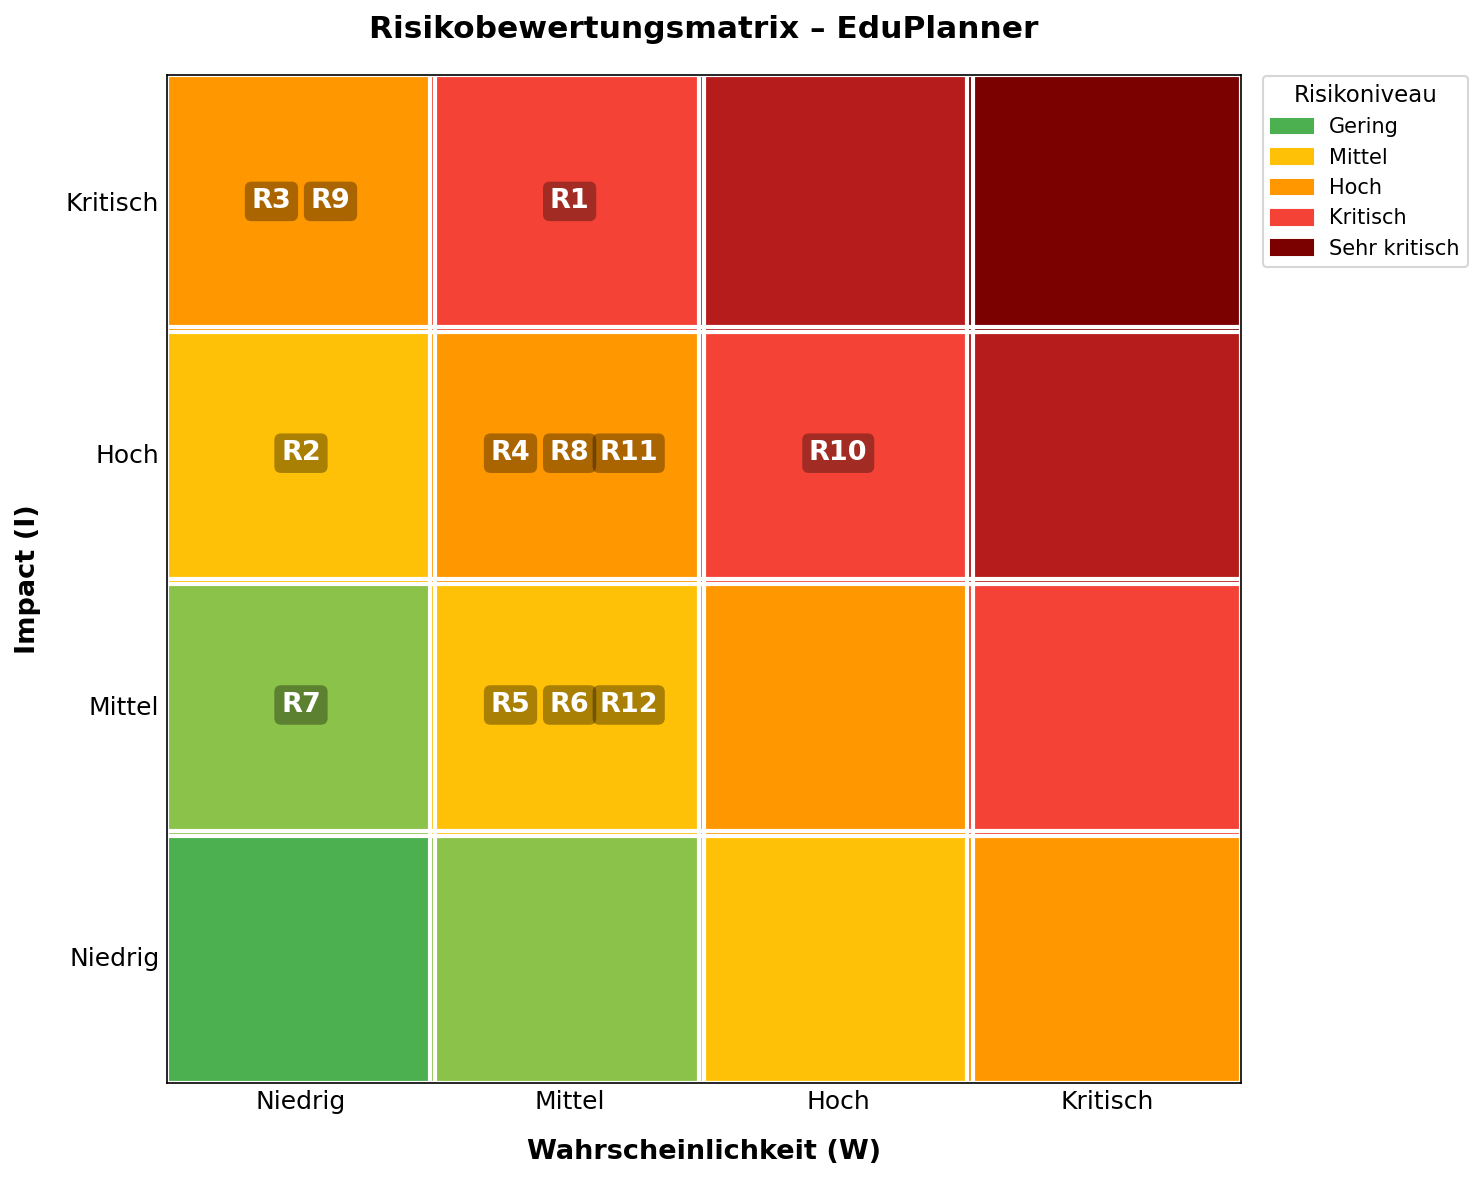
\includegraphics[width=\textwidth]{assets/RiskMatrix}
  \caption{\textit{Risikobewertungsmatrix: Wahrscheinlichkeit vs.\ Impact (R1--R12)}}
  \label{fig:RiskMatrix}
\end{figure}

\textbf{Bewertungsmatrix:} W~=~Wahrscheinlichkeit, I~=~Impact (jeweils: Niedrig / Mittel / Hoch / Kritisch)

\begin{longtable}{C{0.5cm} L{3.5cm} C{1.5cm} C{1.5cm} L{5.5cm}}
  \rowcolor{tableheader}
  \color{white}\textbf{\#} & \color{white}\textbf{Risiko} & \color{white}\textbf{W} & \color{white}\textbf{I} & \color{white}\textbf{Massnahme} \\
  \endfirsthead
  \rowcolor{tableheader}
  \color{white}\textbf{\#} & \color{white}\textbf{Risiko} & \color{white}\textbf{W} & \color{white}\textbf{I} & \color{white}\textbf{Massnahme} \\
  \endhead

  R1 & Race Condition bei Kapazitätsprüfung & Mittel & Kritisch & Optimistic Locking + DB-Unique-Constraint; Lasttests vor Go-Live. Validiert durch Q1. \\
  \rowcolor{tablegrey}
  R2 & RabbitMQ als Single Point of Failure & Niedrig & Hoch & 3-Node Quorum-Cluster; Monitoring; auto.\ Failover getestet. \\
  R3 & Ausfall des Identity Providers & Niedrig & Kritisch & SLA $\geq$ 99,9\,\%; Read-Only-Fallback; JWT-Cache (24\,h). \\
  \rowcolor{tablegrey}
  R4 & PII gelangt in Logs & Mittel & Hoch & Log-Scrubbing; PII-Scanner im CI (detect-secrets). \\
  R5 & Microservice-Overhead überfordert Team & Mittel & Mittel & Modularer Monolith als Fallback definiert; Entscheidung nach MVP. \\
  \rowcolor{tablegrey}
  R6 & Event-Schema-Änderungen brechen Consumer & Mittel & Mittel & Schema Registry evaluieren; nur additive Änderungen. \\
  R7 & Vendor Lock-in & Niedrig & Mittel & Cloud-agnostische Tools (K8s, PostgreSQL, RabbitMQ). \\
  \rowcolor{tablegrey}
  R8 & Key-Person-Abhängigkeit & Mittel & Hoch & Pair-Programming; ADRs als Gedächtnis; Architektur-Workshops. \\
  R9 & DB-Korruption / fehlgeschlagene Migration & Niedrig & Kritisch & Wöchentliche Restore-Tests; Flyway rückwärtskompatibel. \\
  \rowcolor{tablegrey}
  R10 & Team-Burnout \textit{[PM-Risiko]} & Hoch & Hoch & Hiring-Plan Q3; On-Call-Rotation max.\ 1~Wo/Monat. \textit{Anm.: primär Projektmanagement-Risiko, zur Diskussion als Lehrbeispiel.} \\
  R11 & Datenmigration bei Schema-Änderungen & Mittel & Hoch & Expand-Contract-Pattern; Zero-Downtime-Migrations via mehrphasiges Deployment; Staging-Test zwingend. \\
  \rowcolor{tablegrey}
  R12 & Budgetüberschreitung bei Lastspitzen & Mittel & Mittel & Cloud-Kosten variabel bei ungeplantem Traffic. Gegenmassnahme: Reserved Instances für Basisload (CHF~80 Einsparung = 10\,\% Puffer); HPA-Limits verhindern unkontrolliertes Scale-out; monatliches Capacity Review. \\
\end{longtable}

\subsection{Technische Schulden}

Technische Schulden bezeichnen bewusste architektonische Vereinfachungen, die kurzfristig Entwicklungsgeschwindigkeit ermöglichen, langfristig aber Wartungsaufwand oder Sicherheitslücken erzeugen können. Die nachfolgende Tabelle listet alle bekannten Schulden von EduPlanner, bewertet ihre Priorität und definiert einen konkreten Tilgungsplan. Schulden hoher Priorität sind für die nächsten Sprints eingeplant; Schulden niedriger Priorität werden spätestens vor dem v2.0-Release adressiert.

\begin{tabularx}{\textwidth}{C{0.5cm} L{3.5cm} C{1.8cm} X}
  \rowcolor{tableheader}
  \color{white}\textbf{\#} & \color{white}\textbf{Schuld} & \color{white}\textbf{Prio} & \color{white}\textbf{Erläuterung und Tilgungsplan} \\
  TS1 & Kein Service Mesh & Mittel & mTLS intern fehlt. Tilgung: Linkerd in v2.0 (ADR-007). \\
  \rowcolor{tablegrey}
  TS2 & Kein Contract Testing (Pact) & Hoch & API-Kompatibilität manuell koordiniert. Tilgung: Sprint~8. \\
  TS3 & E-Mail-Templates im Container & Niedrig & Änderungen erfordern Re-Deploy. Tilgung: Template-UI in v1.1. \\
  \rowcolor{tablegrey}
  TS4 & Fehlende Multi-Tenancy & Mittel & Single-Tenant (ADR-008). Tilgung: Schema-per-Tenant in v2.0. \\
  TS5 & Kein API-Versionsmanagement $>$~v1 & Niedrig & Tilgung: API-Versionierungsstrategie vor erstem externem API-Zugang -- geplant Sprint~12 (vor v1.0-Release). \\
  \rowcolor{tablegrey}
  TS6 & Keine Accessibility-Tests & Niedrig & WCAG~2.1 AA nicht geprüft. Tilgung: axe-core in v1.1. \\
  TS7 & Rate-Limiting nicht nach Rolle & Niedrig & Alle Rollen gleiche Limits. Tilgung: Kong-Konfig. Sprint~10. \\
\end{tabularx}
\newpage
\section{Glossar}

Das Glossar definiert die Ubiquitous Language von EduPlanner.

\subsection{Fachliche Begriffe}

\begin{longtable}{L{3cm} L{2cm} p{\dimexpr\linewidth-5cm-6\tabcolsep\relax}}
  \rowcolor{tableheader}
  \color{white}\textbf{Begriff} & \color{white}\textbf{Kontext} & \color{white}\textbf{Definition} \\
  \endfirsthead
  \rowcolor{tableheader}
  \color{white}\textbf{Begriff} & \color{white}\textbf{Kontext} & \color{white}\textbf{Definition} \\
  \endhead
 Course & [catalog] & Weiterbildungsangebot mit Titel, Beschreibung und Lernzielen. Beschreibt \emph{was} gelehrt wird. Bsp.: ``Python für Einsteiger''. \\
  \rowcolor{tablegrey}
  CourseStatus & [catalog] & Zustand eines Kurses: DRAFT $\to$ PUBLISHED $\to$ ARCHIVED. Nur diese Übergänge erlaubt (State Machine). \\
  TrainerProfile & [catalog] & Stammdaten eines Trainers inkl.\ Fachgebiete. \\
  \rowcolor{tablegrey}
  CourseExecution & [scheduling] & Konkrete, zeitlich geplante Instanz eines Kurses. Bsp.: ``Python Apr~2025, Bern, max.\ 12~TN''. \\
  ExecutionStatus & [scheduling] & PLANNED $\to$ PUBLISHED $\to$ CANCELLED. Nur PUBLISHED offen für Einschreibungen. \\
  \rowcolor{tablegrey}
  Capacity & [scheduling, reg.] & Maximale Teilnehmeranzahl. Kapazität = 0 $\to$ Warteliste. \\
  Registration & [registration] & Verbindliche Anmeldung eines Teilnehmers zu einer Execution. Bsp.: Max Muster meldet sich an $\to$ \texttt{status=REGISTERED}. \\
  \rowcolor{tablegrey}
  WaitlistEntry & [registration] & Wartelisteneintrag mit Position (1 = erster) und Zeitstempel. \\
  Participant & [identity] & Natürliche Person, die sich einschreiben kann. Systemrolle: PARTICIPANT. \\
  \rowcolor{tablegrey}
  Trainer & [identity] & Kursleiter. Systemrolle: TRAINER. \\
  Staff & [identity] & Mitarbeitende des Kursanbieters. Systemrolle: STAFF. \\
  \rowcolor{tablegrey}
  Admin & [identity] & Nutzer mit erweiterten Systemrechten. Systemrolle: ADMIN. \\
  Domain Event & -- & Unveränderliche Zustandsänderung als Fakt (Vergangenheitsform). Bsp.: \texttt{ParticipantRegistered} (nicht \texttt{RegisterParticipant}). \\
  \rowcolor{tablegrey}
  Bounded Context & -- & Klar abgegrenzter Bereich mit eigener Fachsprache. Bsp.: ``Trainer'' in [catalog] hat andere Bedeutung als in [scheduling]. \\
  Aggregate & -- & Gruppe von Domain-Objekten als konsistente Einheit. Aggregate Root ist einziger Einstiegspunkt. Bsp.: Registration-Aggregate verhindert Überbuchung. \\
  \rowcolor{tablegrey}
  Ubiquitous Language & -- & Gemeinsame fachliche Sprache innerhalb eines BC. Code-Bezeichner verwenden exakt dieselben Begriffe wie die Fachsprache. \\
\end{longtable}

\subsection{Domain Events -- Vollständige Übersicht}

\begin{tabularx}{\textwidth}{L{5cm} L{2.5cm} X}
  \rowcolor{tableheader}
  \color{white}\textbf{Domain Event} & \color{white}\textbf{Kontext} & \color{white}\textbf{Auslöser} \\
  CourseCreated & catalog & Staff legt Kurs an \\
  \rowcolor{tablegrey}
  CourseTitleUpdated & catalog & Staff aktualisiert Kurstitel \\
  TrainerAssignedToCourse & catalog & Staff ordnet Trainer zu \\
  \rowcolor{tablegrey}
  CoursePublished & catalog & Admin veröffentlicht \\
  CourseArchived & catalog & Admin archiviert \\
  \rowcolor{tablegrey}
  CourseExecutionScheduled & scheduling & Staff plant Durchführung \\
  TrainerAssignedToExecution & scheduling & Staff weist Trainer zu \\
  \rowcolor{tablegrey}
  CourseExecutionPublished & scheduling & Admin gibt frei \\
  CourseExecutionCancelled & scheduling & Admin / System storniert \\
  \rowcolor{tablegrey}
  ParticipantRegistered & registration & Teilnehmer schreibt sich ein \\
  ParticipantAddedToWaitlist & registration & Kurs voll \\
  \rowcolor{tablegrey}
  RegistrationCancelled & registration & Teilnehmer / Staff storniert \\
  WaitlistParticipantPromoted & registration & Nachrücker von Warteliste \\
  \rowcolor{tablegrey}
  EmailNotificationSent & notification & System hat E-Mail versendet \\
  UserCreated & identity & Admin / IdP legt Benutzer an \\
  \rowcolor{tablegrey}
  UserRoleAssigned & identity & Admin weist Rolle zu \\
\end{tabularx}

\newpage
\section{Betrieb und Deployment -- Runbook}

\begin{hinweis}[Erweiterung des arc42-Templates]
Dieses Kapitel ist \emph{keine} Bestandteil des offiziellen arc42-Templates~v9,
das mit Kapitel~12 (Glossar) endet. Es ergänzt die Architekturdokumentation um
operative Aspekte, die für den produktiven Betrieb von EduPlanner notwendig sind.
In einem realen Projekt würde dieses Runbook typischerweise als eigenständiges
Dokument (z.\,B.\ im Team-Wiki) gepflegt und laufend aktualisiert.
\end{hinweis}

Dieses Kapitel dient als operatives Nachschlagewerk für den laufenden Betrieb von EduPlanner. Es beschreibt verbindliche Checklisten vor jedem Deployment, definiert Reaktionszeiten und Eskalationsstufen für Incidents sowie die regelmässig anfallenden Wartungsarbeiten. Das Runbook richtet sich an das Entwicklungs- und Betriebsteam und ist bei jeder Änderung am Deploymentprozess aktuell zu halten.

\subsection{Pre-Deployment Checklist}

Vor jedem produktiven Deployment ist die nachfolgende Checkliste vollständig abzuarbeiten. Kein Deployment darf ohne grüne CI-Pipeline und dokumentierten Rollback-Plan erfolgen. Bei Breaking Changes gegenüber bestehenden API-Konsumenten ist zusätzlich die frühzeitige Stakeholder-Kommunikation obligatorisch.

\begin{tabularx}{\textwidth}{C{0.6cm} X}
  \rowcolor{tableheader}
  \color{white}\textbf{\#} & \color{white}\textbf{Prüfpunkt} \\
  1 & Code Review abgeschlossen (min.\ 1~Approval) \\
  \rowcolor{tablegrey}
  2 & Alle Unit- und Integrationstests grün (CI~Pipeline) \\
  3 & Security Scan erfolgreich (Trivy: keine Critical/High) \\
  \rowcolor{tablegrey}
  4 & Schema-Migration in Staging getestet (Flyway dryrun) \\
  5 & OpenAPI-Spezifikation aktualisiert (falls API-Änderung) \\
  \rowcolor{tablegrey}
  6 & Pact Contract Tests grün (ab Sprint~8) \\
  7 & Docker Image mit Immutable Tag (Git SHA) \\
  \rowcolor{tablegrey}
  8 & Release Notes erstellt \\
  9 & Rollback-Plan dokumentiert \\
  \rowcolor{tablegrey}
  10 & Stakeholder informiert (bei Breaking Changes) \\
\end{tabularx}

\subsection{Incident Response}

Tritt ein Störfall auf, wird dieser anhand der nachfolgenden Severity-Stufen klassifiziert. Die Einstufung bestimmt die maximale Reaktionszeit sowie den Eskalationspfad. SEV-1- und SEV-2-Incidents sind umgehend im internen Kommunikationskanal zu melden; für SEV-1 gilt zusätzlich die sofortige Benachrichtigung der Projektleitung. Nach jedem SEV-1- oder SEV-2-Incident ist ein Post-Mortem-Bericht innerhalb von 48~Stunden zu erstellen.

\begin{tabularx}{\textwidth}{C{1.5cm} L{3.5cm} C{2.2cm} X}
  \rowcolor{tableheader}
  \color{white}\textbf{Severity} & \color{white}\textbf{Beschreibung} & \color{white}\textbf{Reaktionszeit} & \color{white}\textbf{Beispiele} \\
  SEV-1 & System nicht verfügbar & 15~min & Komplettausfall; Datenverlust; Sicherheitsvorfall \\
  \rowcolor{tablegrey}
  SEV-2 & Kernfunktion eingeschränkt & 1~h & Einschreibungen nicht möglich \\
  SEV-3 & Nicht-kritische Funktion & 4~h & E-Mail-Versand verzögert \\
  \rowcolor{tablegrey}
  SEV-4 & Kosmetisch / Minor & Nächster Sprint & UI-Darstellungsfehler \\
\end{tabularx}

\subsection{Routine-Wartungsarbeiten}

Neben dem reaktiven Incident-Management sind folgende Wartungsarbeiten proaktiv und nach festgelegtem Rhythmus durchzuführen. Sie dienen der langfristigen Systemstabilität, der Datensicherheit und der Kostenkontrolle. Die Verantwortung für die termingerechte Durchführung liegt beim jeweils zuständigen Teammitglied; die Ergebnisse sind im internen Betriebslog zu dokumentieren.

\begin{tabularx}{\textwidth}{L{3.5cm} L{2.5cm} X}
  \rowcolor{tableheader}
  \color{white}\textbf{Aufgabe} & \color{white}\textbf{Frequenz} & \color{white}\textbf{Beschreibung} \\
  DB-Backup-Validierung & Wöchentlich & Auto-Restore in Testing; Datenintegrität validieren \\
  \rowcolor{tablegrey}
  Dependency Updates & 2-wöchentlich & Dependabot PRs; Security Patches priorisieren \\
  Certificate Renewal & Monatlich prüfen & Let's Encrypt autorenew; 30~Tage vor Ablauf prüfen \\
  \rowcolor{tablegrey}
  Capacity Review & Monatlich & Cloud-Kosten; Reserved Instances evaluieren \\
  Security Scan & Wöchentlich & Trivy, Snyk \\
  \rowcolor{tablegrey}
  Chaos Engineering & Wöchentlich & Pod-Kills, Network-Delays in Staging \\
  DR-Systemtest & Halbjährlich & Vollständiger Failover-Test; Verantwortung: Patrick Hari \\
\end{tabularx}
\newpage
\section{Roadmap und Evolution}

\begin{hinweis}[Erweiterung des arc42-Templates]
Auch dieses Kapitel ist \emph{kein} Bestandteil des offiziellen arc42-Templates~v9.
Zukunftspläne und technische Weiterentwicklung sind im arc42-Standard unter
Kapitel~11 (Risiken und technische Schulden) angesiedelt. Eine dedizierte Roadmap
geht darüber hinaus und ist hier als Lehrbeispiel für die Planung von
Architekturevolution dokumentiert. In der Praxis lebt ein solches Dokument
typischerweise als Product-Roadmap im Projektmanagement-Tool (z.\,B.\ Jira, Linear).
\end{hinweis}

Dieses Kapitel beschreibt die geplante Entwicklung von EduPlanner über die kommenden Versionen. Die Roadmap orientiert sich an den identifizierten technischen Schulden (Kap.~11), den Qualitätszielen (Kap.~10) sowie den geschäftlichen Anforderungen. Die Umsetzung beginnt im April~2026; alle Zeitangaben sind als Planungsziele zu verstehen und werden im Rahmen des regulären Sprint-Reviews angepasst.

\subsection{Versionsübersicht}

Die folgende Tabelle gibt einen kompakten Überblick über alle geplanten Versionen und ihre zentralen Meilensteine. Die Versionen bauen aufeinander auf: Das MVP legt die technische Basis, v1.0 konsolidiert und stabilisiert, v1.1 tilgt priorisierte technische Schulden, und v2.0 transformiert EduPlanner zu einer mandantenfähigen SaaS-Plattform.

\begin{tabularx}{\textwidth}{L{2.5cm} C{2.5cm} X}
  \rowcolor{tableheader}
  \color{white}\textbf{Version} & \color{white}\textbf{Zeitraum} & \color{white}\textbf{Meilenstein} \\
  MVP (v0.1--v0.9) & Q2 2026 & Kernfunktionen: Katalog, Einschreibung, E-Mail, RBAC \\
  \rowcolor{tablegrey}
  v1.0 & Q3 2026 & Vollständiger Release: API-Doku, Performance-Tests, Security-Audit \\
  v1.1 & Q4 2026 & Polish: Contract Tests, Template-UI, Accessibility, Rate-Limiting \\
  \rowcolor{tablegrey}
  v2.0 & Q1--Q2 2027 & SaaS / Multi-Tenancy: Schema-per-Tenant, Service Mesh, Payment \\
\end{tabularx}

\subsection{v1.1 -- Polish und Stabilität (Q4 2026)}

Version~1.1 fokussiert sich auf die Tilgung der höchstpriorisierten technischen Schulden aus Kap.~11 sowie auf eine verbesserte Nutzererfahrung. Die in dieser Phase umgesetzten Massnahmen sind Voraussetzung für den stabilen Betrieb und bilden die Basis für die umfangreichen Erweiterungen in v2.0. Alle Punkte sind bereits in der Backlog-Priorisierung berücksichtigt.

\begin{tabularx}{\textwidth}{C{0.8cm} L{4cm} X}
  \rowcolor{tableheader}
  \color{white}\textbf{\#} & \color{white}\textbf{Feature / Tilgung} & \color{white}\textbf{Details} \\
  TS2 & Contract Testing & Pact-Tests für alle Service-Schnittstellen \\
  \rowcolor{tablegrey}
  TS3 & Template-Management-UI & E-Mail-Templates über Admin-UI konfigurierbar \\
  TS6 & Accessibility & axe-core in Cypress; WCAG~2.1~AA \\
  \rowcolor{tablegrey}
  TS7 & Differenziertes Rate-Limiting & Unterschiedliche Limits pro Rolle \\
  -- & iCal-Export & Durchführungstermine als iCal-Feed \\
\end{tabularx}

\subsection{v2.0 -- Multi-Tenancy und SaaS (Q1--Q2 2027)}

Version~2.0 stellt den grössten Evolutionsschritt von EduPlanner dar: Die Plattform wird von einer Single-Tenant-Applikation zu einer vollwertigen SaaS-Lösung mit Mandantenfähigkeit weiterentwickelt. Diese Phase erfordert tiefgreifende Änderungen an Datenbankschicht, Authentifizierung und Infrastruktur. R11 (Datenmigration, Kap.~11.1) ist das grösste Risiko dieser Phase und wird durch das Expand-Contract-Pattern sowie zwingende Staging-Tests mitigiert.

\begin{korrektur}[Architekturhinweis v2.0]
  v2.0 erfordert signifikante Änderungen an der Datenbankschicht (ADR-008~Tilgung) und der Authentifizierung.
  R11 (Datenmigration) ist das grösste Risiko dieser Phase.
\end{korrektur}

\begin{tabularx}{\textwidth}{L{3.5cm} X}
  \rowcolor{tableheader}
  \color{white}\textbf{Feature} & \color{white}\textbf{Beschreibung} \\
  Multi-Tenancy & Schema-per-Tenant; \texttt{tenant\_id} in allen Tabellen; Tenant-Routing; separates IdP-Realm. (Tilgung TS4, ADR-008) \\
  \rowcolor{tablegrey}
  Service Mesh & Linkerd für mTLS, L7-Observability, auto.\ Retry. (Tilgung TS1, ADR-007) \\
  Payment Gateway & Stripe-Integration; Rechnungsstellung; Gutschein-System. \\
  \rowcolor{tablegrey}
  Mobile App & React~Native für iOS/Android; Push-Notifications. \\
  Advanced Analytics & Data Warehouse; BI-Dashboard; ML-Kursempfehlungen. \\
  \rowcolor{tablegrey}
  LMS-Integration & API-Schnittstellen zu Moodle, Canvas. \\
  GraphQL API & Optionale GraphQL-Schicht neben REST. \\
\end{tabularx}
\newpage

% ── ANHANG & REFERENZEN ───────────────────────────────────────
\appendix
\section{Anhang~A: Event~Storming -- Ergebnisse}

Dieser Anhang dokumentiert die Ergebnisse des Event-Storming-Workshops, der zu Beginn der Architekturarbeit durchgeführt wurde. Event~Storming\footnote{%
  \textit{Event Storming} wurde von Alberto Brandolini entwickelt und erstmals in seinem Buch
  \textit{Introducing EventStorming} (Leanpub, 2021, \url{https://leanpub.com/introducing_eventstorming})
  beschrieben. Weitere Informationen unter \url{https://www.eventstorming.com}.}
ist eine kollaborative Workshop-Technik aus dem Domain-Driven Design (DDD), bei der Fachexperten und Entwickler gemeinsam die relevanten Ereignisse (Events) eines Geschäftsbereichs auf farbcodierten Haftnotizen erarbeiten. Ziel ist es, ein gemeinsames Verständnis der Domäne zu schaffen, Bounded~Contexts zu identifizieren und die Grundlage für eine ereignisorientierte Architektur zu legen -- ohne technische Implementierungsdetails vorwegzunehmen.

\subsection{Methodik}

Das Event~Storming wurde nach der Methode von Alberto Brandolini durchgeführt. Der Workshop gliedert sich in sechs aufeinander aufbauende Phasen, die vom bewusst unstrukturierten Sammeln von Ereignissen bis hin zur Identifikation fachlicher Grenzen (Bounded~Contexts) führen.

\begin{enumerate}[leftmargin=2em]
  \item \textbf{Chaotische Exploration} ($\sim$30~min): Alle Teilnehmer schreiben Domain~Events auf orangefarbene Haftnotizen.
  \item \textbf{Timeline}: Events werden in zeitlicher Reihenfolge angeordnet.
  \item \textbf{Hotspots}: Rote Karten für unklare Stellen.
  \item \textbf{Kommandos}: Blaue Karten für Nutzeraktionen vor dem Event.
  \item \textbf{Akteure und Systeme}: Gelbe Karten für Auslöser.
  \item \textbf{Bounded Contexts}: Natürliche Gruppen werden eingerahmt.
\end{enumerate}

\subsection{Vollständige Domain-Event-Liste}

Die nachfolgende Tabelle listet alle im Workshop erarbeiteten Domain~Events von EduPlanner. Jedes Event ist einem auslösenden Akteur (Staff, Admin, Participant oder System) sowie einem Bounded~Context zugeordnet. Die Bounded~Contexts entsprechen direkt den Microservices der Zielarchitektur (vgl.\ Kap.~5).

\begin{tabularx}{\textwidth}{L{5cm} L{3.5cm} X}
  \rowcolor{tableheader}
  \color{white}\textbf{Domain Event} & \color{white}\textbf{Auslöser (Akteur)} & \color{white}\textbf{Bounded Context} \\
  CourseCreated & Staff & catalog \\
  \rowcolor{tablegrey}
  CourseTitleUpdated & Staff & catalog \\
  TrainerAssignedToCourse & Staff & catalog \\
  \rowcolor{tablegrey}
  CoursePublished & Admin & catalog \\
  CourseArchived & Admin & catalog \\
  \rowcolor{tablegrey}
  CourseExecutionScheduled & Staff & scheduling \\
  TrainerAssignedToExecution & Staff & scheduling \\
  \rowcolor{tablegrey}
  CourseExecutionPublished & Admin & scheduling \\
  CourseExecutionCancelled & Admin / System & scheduling \\
  \rowcolor{tablegrey}
  ParticipantRegistered & Participant & registration \\
  ParticipantAddedToWaitlist & System & registration \\
  \rowcolor{tablegrey}
  RegistrationCancelled & Participant / Staff & registration \\
  WaitlistParticipantPromoted & System & registration \\
  \rowcolor{tablegrey}
  EmailNotificationSent & System & notification \\
  UserCreated & Admin / IdP & identity \\
  \rowcolor{tablegrey}
  UserRoleAssigned & Admin & identity \\
\end{tabularx}
\newpage
% ============================================================
% ANHANG B – Diagramme in A4 Querformat (Grossansicht)
% ============================================================
% Voraussetzung im Preamble: \usepackage{pdflscape}
% ============================================================

\section{Anhang~B: Diagramme in A4\,Quer -- Grossansicht}
\label{sec:anhang-diagramme}

\begin{hinweis}[Hinweis zur Lesbarkeit]
Die folgenden Diagramme sind identisch mit den im Fliesstext eingebetteten
Abbildungen, werden hier jedoch auf A4-Querformat dargestellt, um die
Detaillesbarkeit zu verbessern.
\end{hinweis}

% ── C4 Kontextdiagramm ──────────────────────────────────────
\begin{landscape}
\begin{figure}[p]
  \centering
  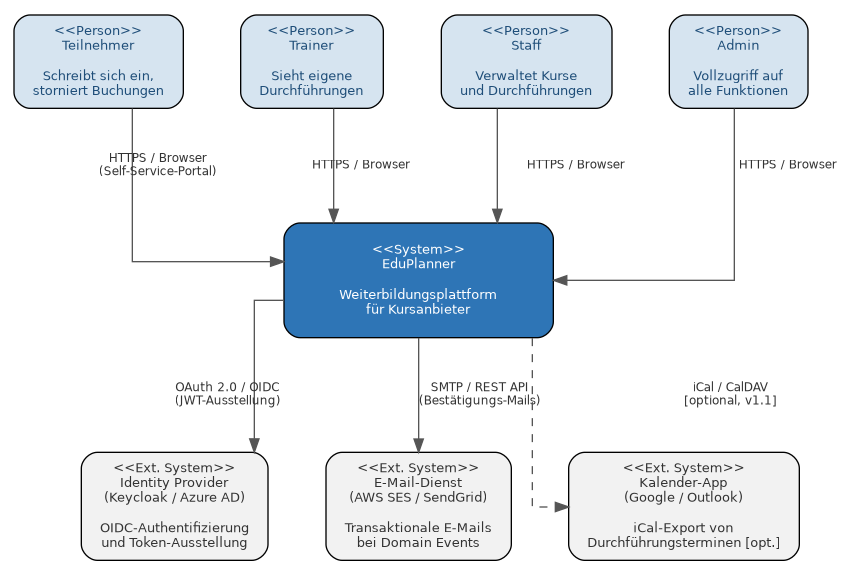
\includegraphics[width=0.95\linewidth]{assets/context_diagram}
  \caption{Grossansicht -- \textit{C4-Kontextdiagramm EduPlanner}
    (vgl.\ Kap.~3.1, Abb.~\ref{fig:context_diagram})}
\end{figure}
\end{landscape}

% ── DDD Context Map ─────────────────────────────────────────
\begin{landscape}
\begin{figure}[p]
  \centering
  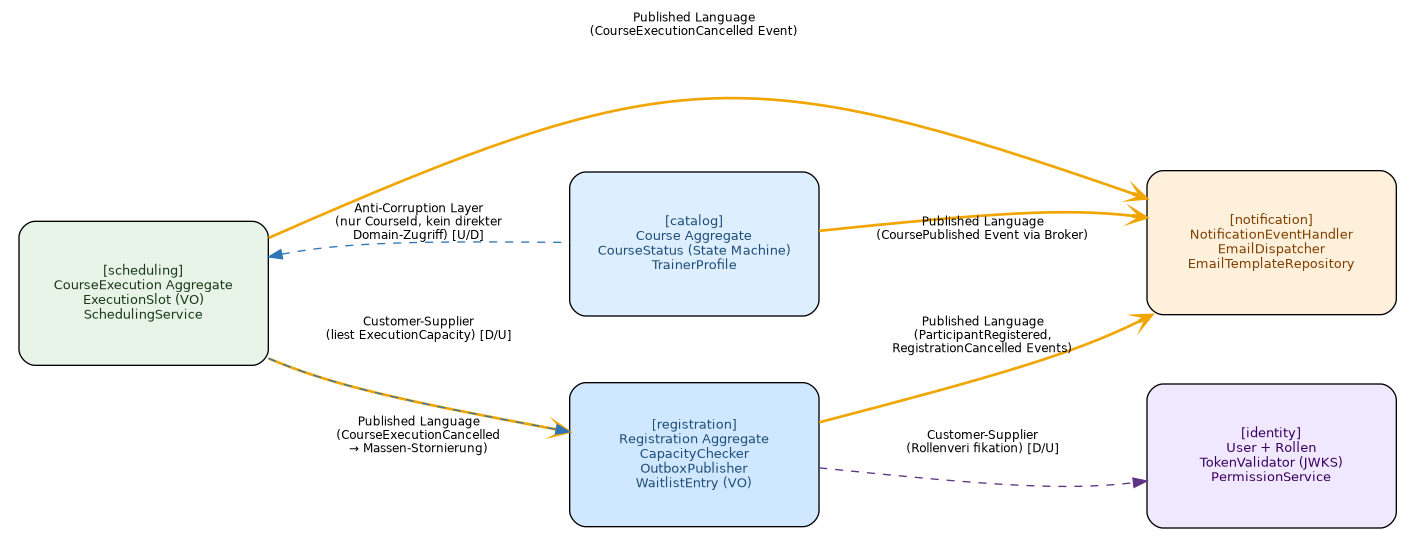
\includegraphics[width=0.95\linewidth]{assets/context_map}
  \caption{Grossansicht -- \textit{DDD Context Map: Bounded Contexts und Beziehungen}
    (vgl.\ Kap.~4.2.2, Abb.~\ref{fig:context_map})}
\end{figure}
\end{landscape}

% ── C4 Container Diagramm (Ebene 1) ─────────────────────────
\begin{landscape}
\begin{figure}[p]
  \centering
  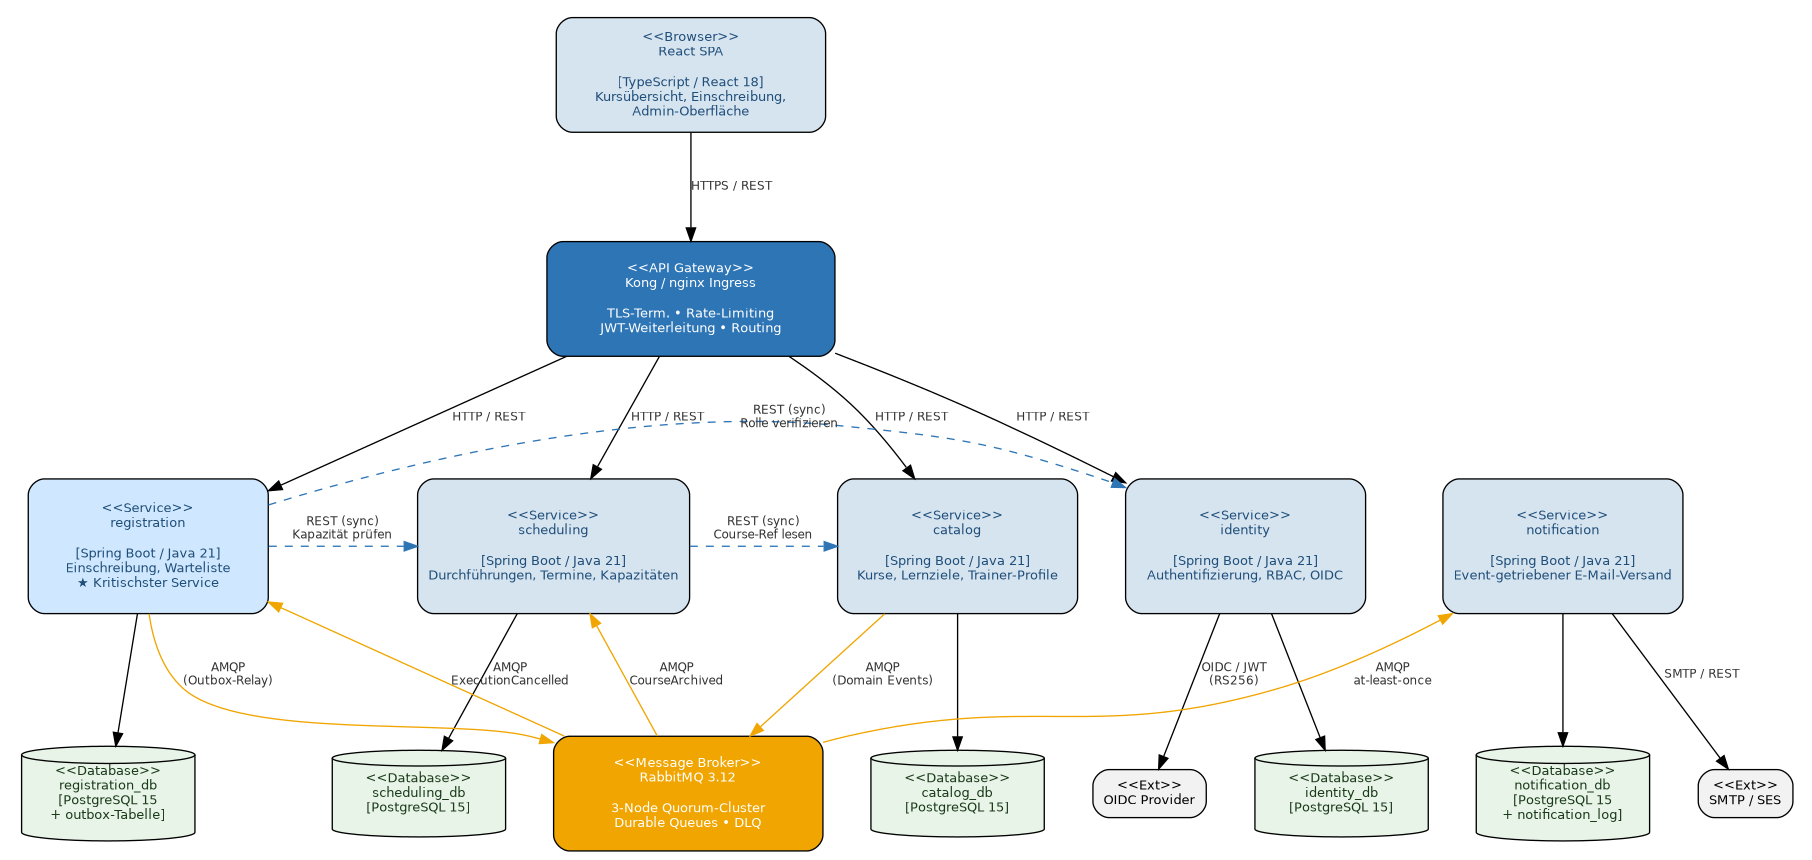
\includegraphics[width=0.95\linewidth]{assets/ebene1_container_diagram}
  \caption{Grossansicht -- \textit{C4-Container-Diagramm: Gesamtsystem EduPlanner}
    (vgl.\ Kap.~5.1, Abb.~\ref{fig:container})}
\end{figure}
\end{landscape}

% ── catalog Service ──────────────────────────────────────────
\begin{landscape}
\begin{figure}[p]
  \centering
  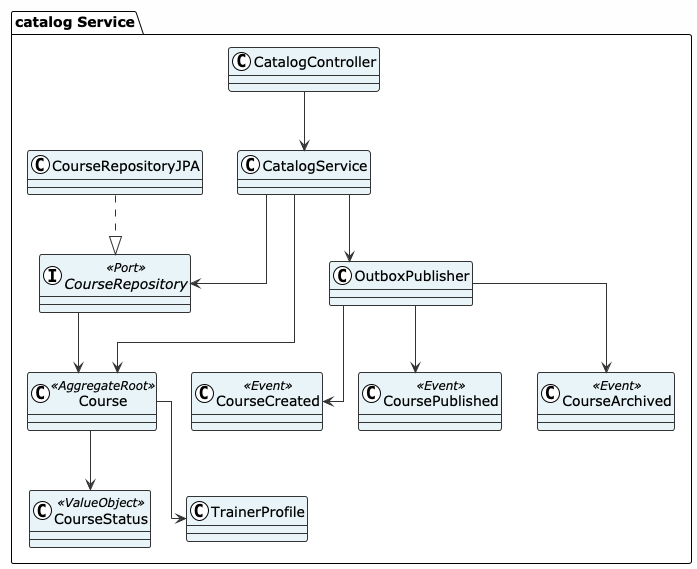
\includegraphics[width=0.85\linewidth]{assets/ebene2_catalog_class_diagram}
  \caption{Grossansicht -- \textit{UML-Klassendiagramm: \texttt{catalog}-Service}
    (vgl.\ Kap.~5.2, Abb.~\ref{fig:catalog})}
\end{figure}
\end{landscape}

% ── CourseStatus Zustandsdiagramm ───────────────────────────
\begin{landscape}
\begin{figure}[p]
  \centering
  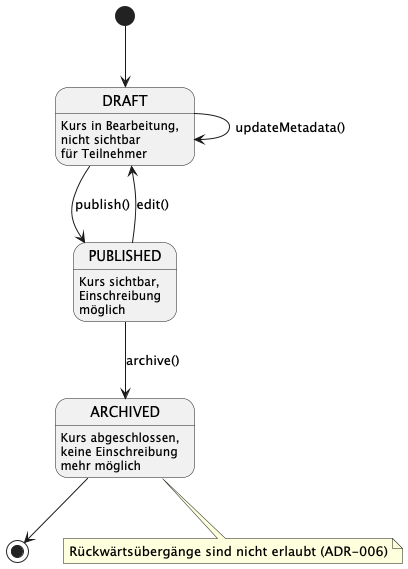
\includegraphics[width=0.70\linewidth]{assets/catalog_course_state_machine}
  \caption{Grossansicht -- \textit{Zustandsübergangsdiagramm \texttt{CourseStatus}}
    (vgl.\ Kap.~5.2.1, Abb.~\ref{fig:course-state})}
\end{figure}
\end{landscape}

% ── scheduling Service ───────────────────────────────────────
\begin{landscape}
\begin{figure}[p]
  \centering
  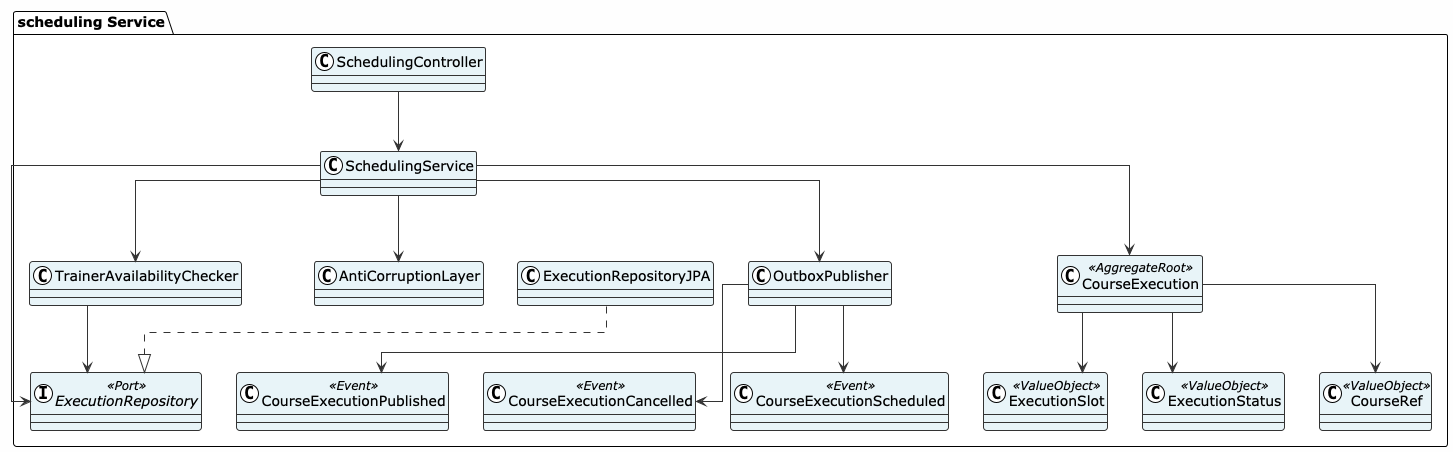
\includegraphics[width=0.95\linewidth]{assets/ebene2_scheduling_class_diagram}
  \caption{Grossansicht -- \textit{UML-Klassendiagramm: \texttt{scheduling}-Service
    inkl.\ Anti-Corruption Layer}
    (vgl.\ Kap.~5.3, Abb.~\ref{fig:scheduling})}
\end{figure}
\end{landscape}

% ── registration Service ─────────────────────────────────────
\begin{landscape}
\begin{figure}[p]
  \centering
  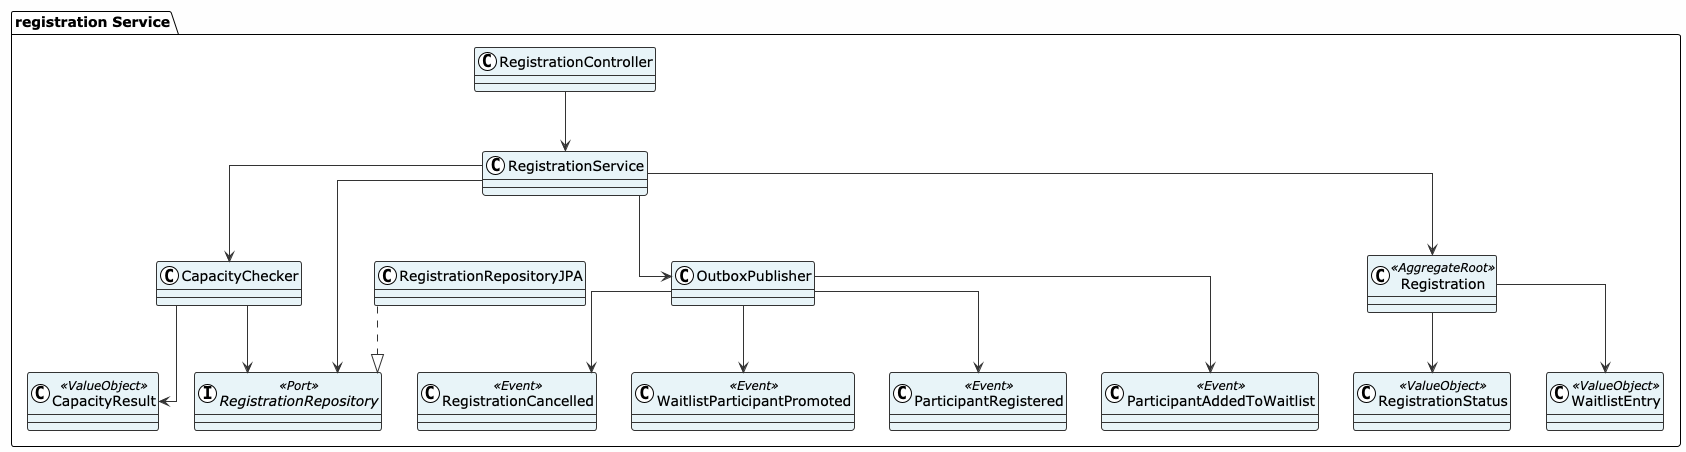
\includegraphics[width=0.95\linewidth]{assets/ebene2_registration_class_diagram}
  \caption{Grossansicht -- \textit{UML-Klassendiagramm: \texttt{registration}-Service}
    (vgl.\ Kap.~5.4, Abb.~\ref{fig:registration})}
\end{figure}
\end{landscape}

% ── notification Service ─────────────────────────────────────
\begin{landscape}
\begin{figure}[p]
  \centering
  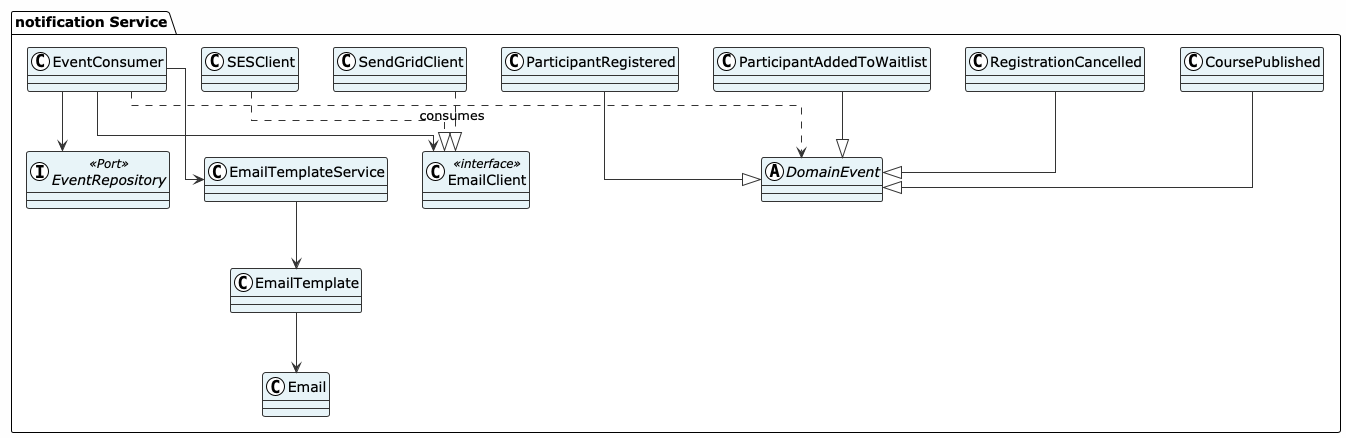
\includegraphics[width=0.85\linewidth]{assets/ebene2_notification_class_diagram}
  \caption{Grossansicht -- \textit{UML-Klassendiagramm: \texttt{notification}-Service}
    (vgl.\ Kap.~5.5, Abb.~\ref{fig:notification})}
\end{figure}
\end{landscape}

% ── identity Service ─────────────────────────────────────────
\begin{landscape}
\begin{figure}[p]
  \centering
  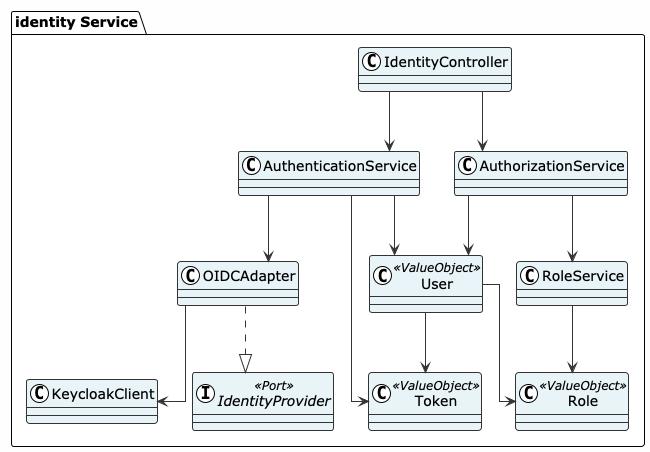
\includegraphics[width=0.85\linewidth]{assets/ebene2_identity_class_diagram}
  \caption{Grossansicht -- \textit{UML-Klassendiagramm: \texttt{identity}-Service}
    (vgl.\ Kap.~5.6, Abb.~\ref{fig:identity})}
\end{figure}
\end{landscape}

% ── Sequenzdiagramm 1 ────────────────────────────────────────
\begin{landscape}
\begin{figure}[p]
  \centering
  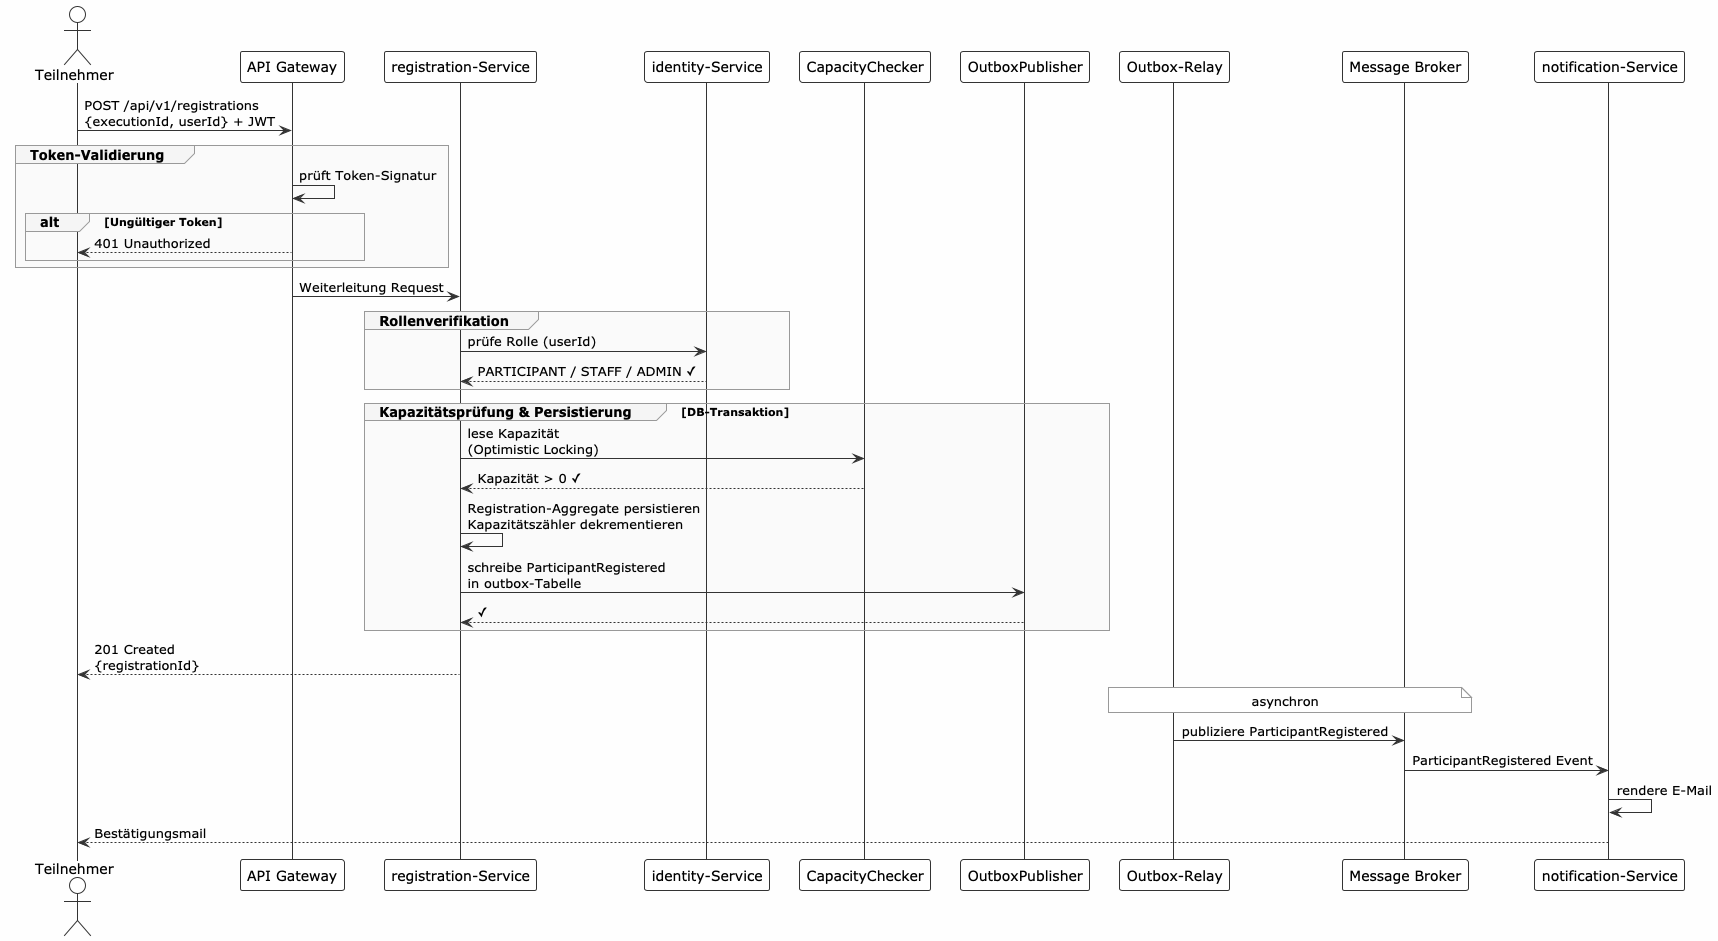
\includegraphics[width=0.95\linewidth]{assets/sequence_diagram_1}
  \caption{Grossansicht -- \textit{Szenario~1: Teilnehmer schreibt sich ein (Happy Path)}
    (vgl.\ Kap.~6.1, Abb.~\ref{fig:sequence_diagram_1})}
\end{figure}
\end{landscape}

% ── Sequenzdiagramm 2 ────────────────────────────────────────
\begin{landscape}
\begin{figure}[p]
  \centering
  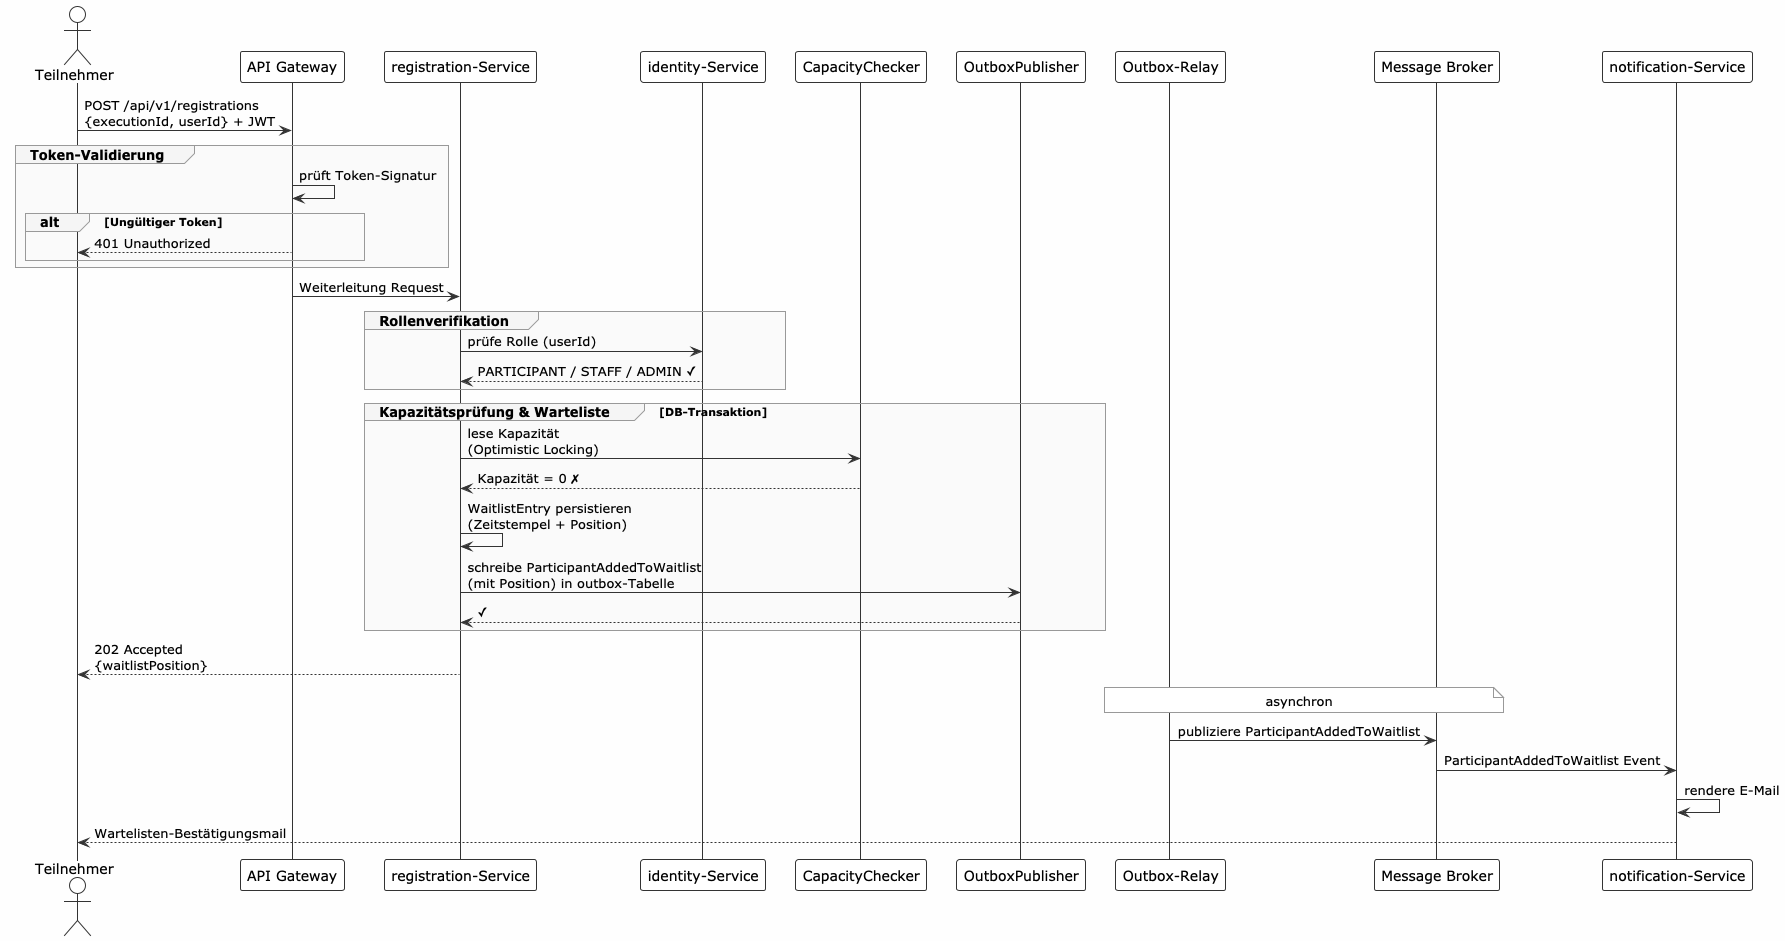
\includegraphics[width=0.95\linewidth]{assets/sequence_diagram_2}
  \caption{Grossansicht -- \textit{Szenario~2: Kurs ausgebucht -- Warteliste}
    (vgl.\ Kap.~6.2, Abb.~\ref{fig:sequence_diagram_2})}
\end{figure}
\end{landscape}

% ── Sequenzdiagramm 3 ────────────────────────────────────────
\begin{landscape}
\begin{figure}[p]
  \centering
  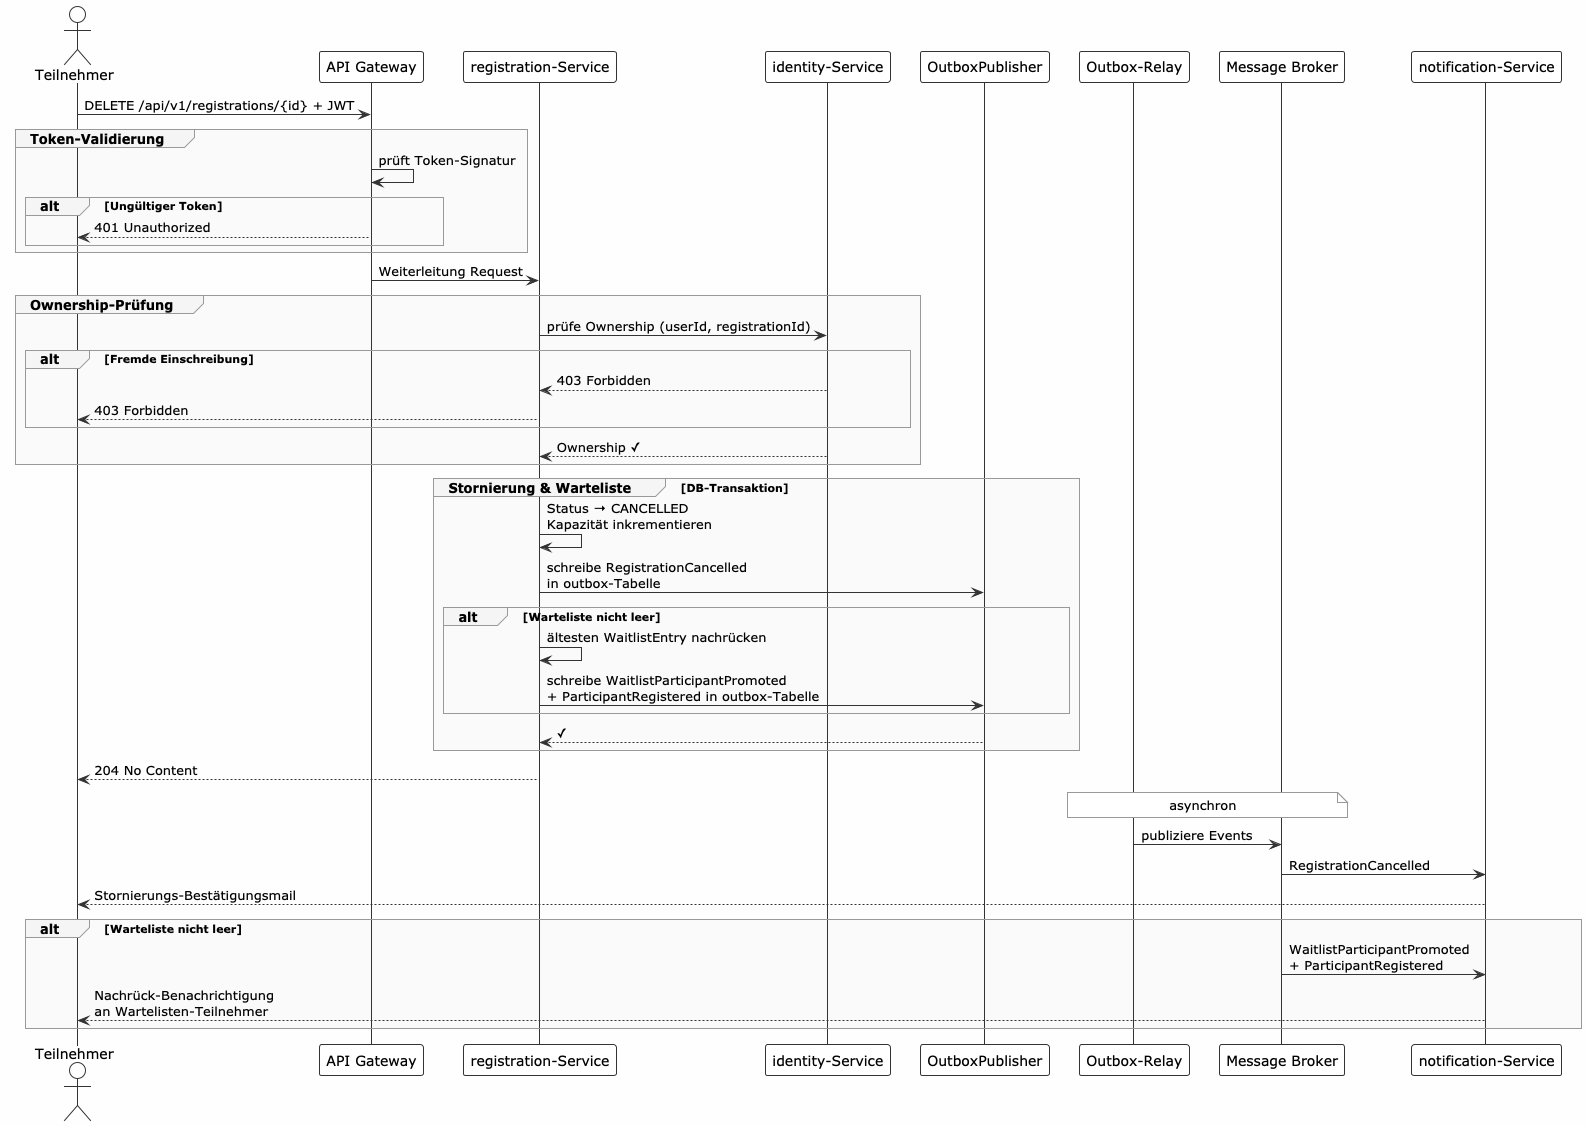
\includegraphics[width=0.95\linewidth]{assets/sequence_diagram_3}
  \caption{Grossansicht -- \textit{Szenario~3: Einschreibung stornieren}
    (vgl.\ Kap.~6.3, Abb.~\ref{fig:sequence_diagram_3})}
\end{figure}
\end{landscape}

% ── Sequenzdiagramm 4 ────────────────────────────────────────
\begin{landscape}
\begin{figure}[p]
  \centering
  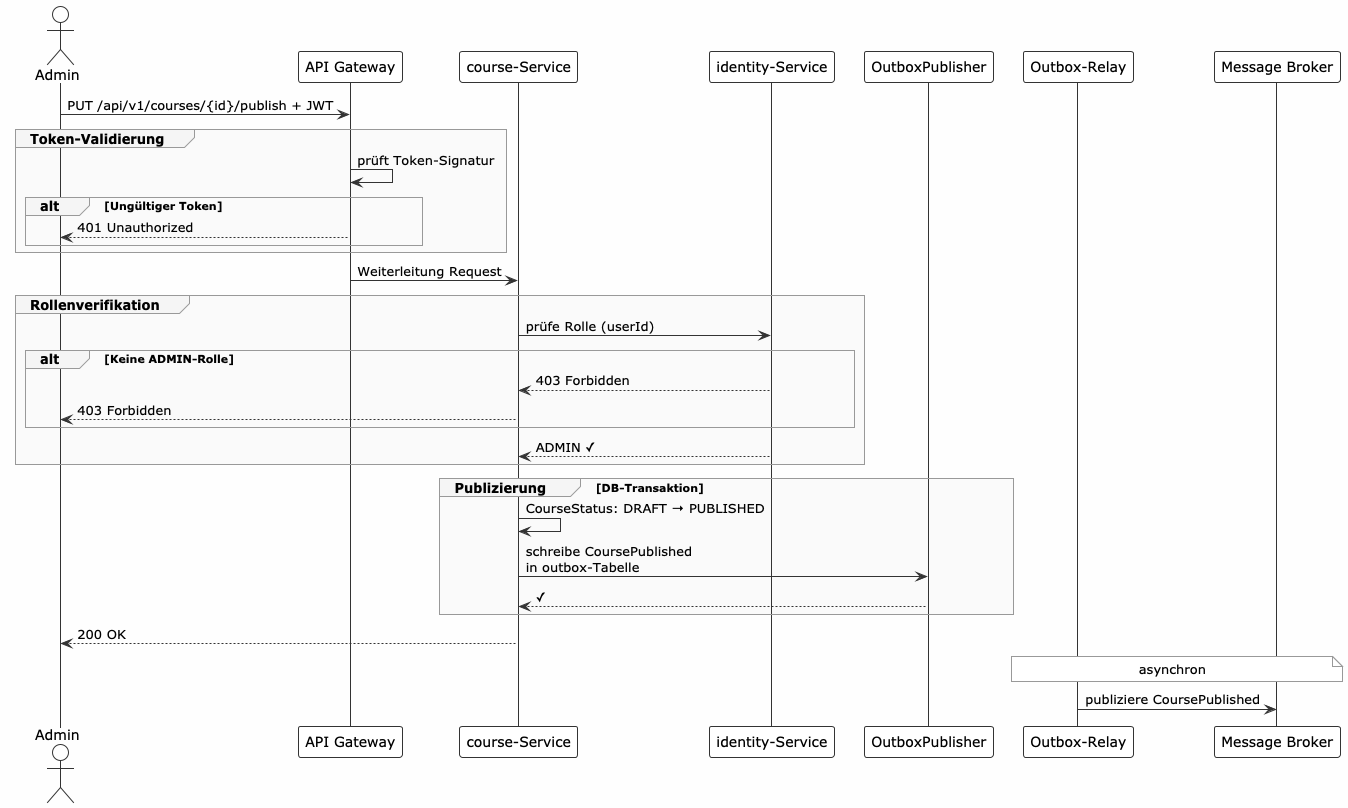
\includegraphics[width=0.95\linewidth]{assets/sequence_diagram_4}
  \caption{Grossansicht -- \textit{Szenario~4: Admin veröffentlicht einen Kurs}
    (vgl.\ Kap.~6.4, Abb.~\ref{fig:sequence_diagram_4})}
\end{figure}
\end{landscape}

% ── Sequenzdiagramm 5 ────────────────────────────────────────
\begin{landscape}
\begin{figure}[p]
  \centering
  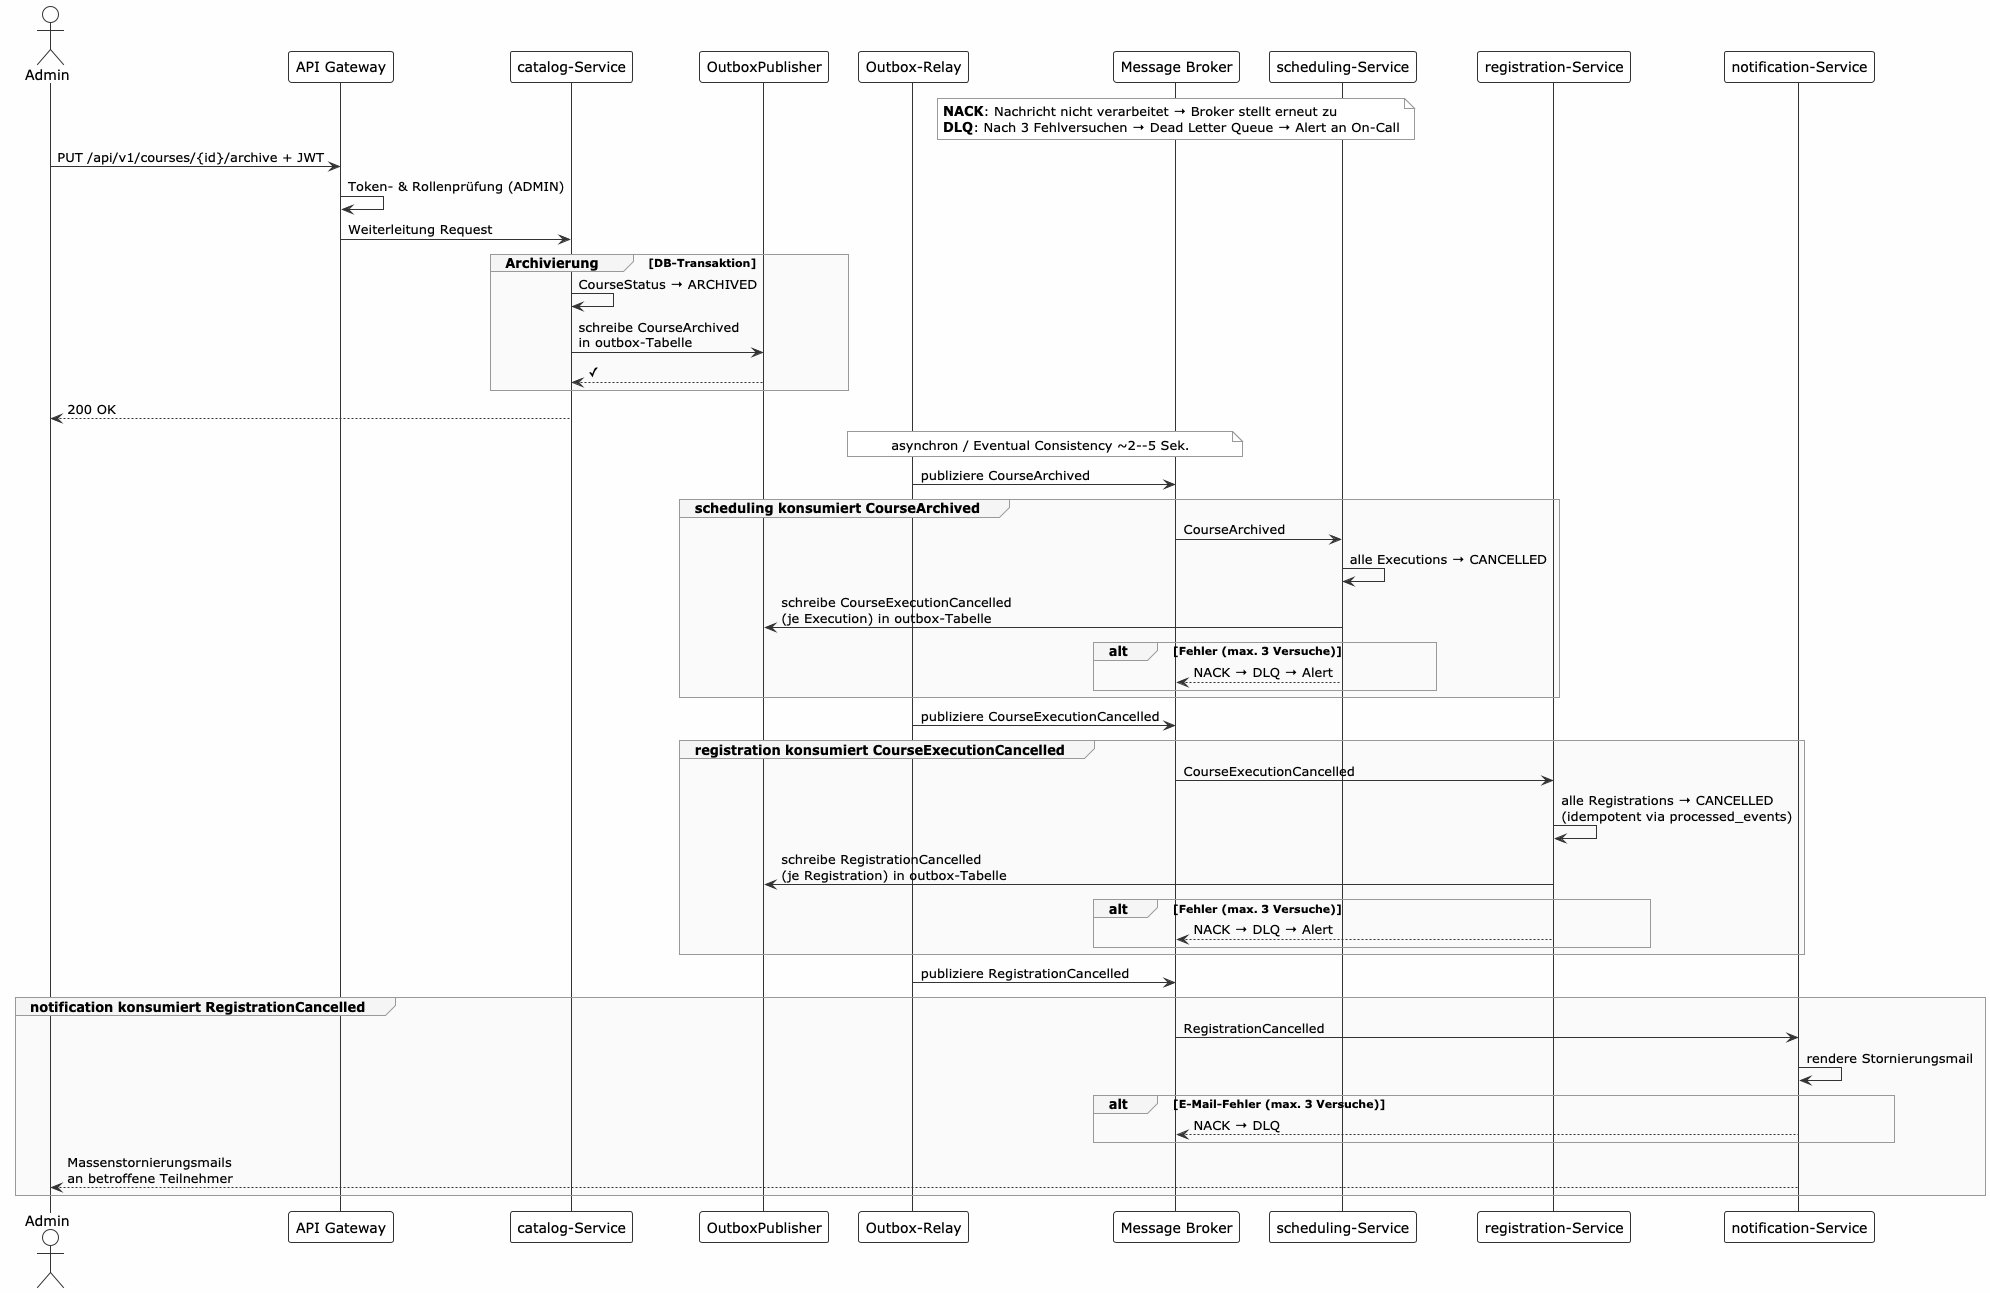
\includegraphics[width=0.95\linewidth]{assets/sequence_diagram_5}
  \caption{Grossansicht -- \textit{Szenario~5: Cross-Context-Transaktion (Kurs archivieren)}
    (vgl.\ Kap.~6.5, Abb.~\ref{fig:sequence_diagram_5})}
\end{figure}
\end{landscape}

% ── Deployment-Diagramm ──────────────────────────────────────
\begin{landscape}
\begin{figure}[p]
  \centering
  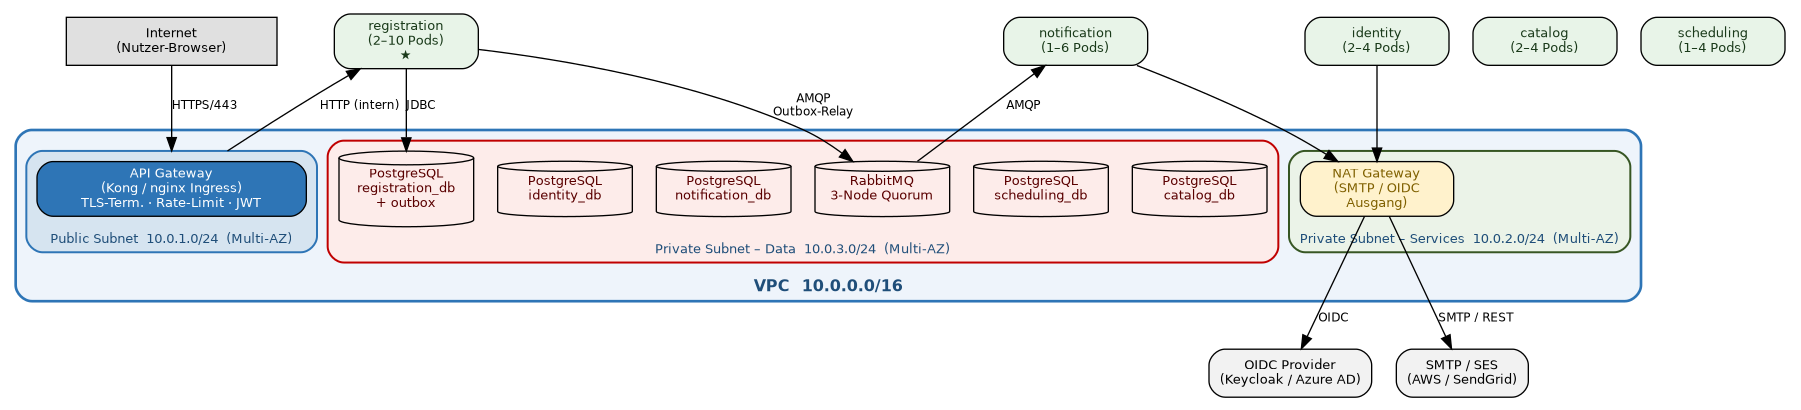
\includegraphics[width=0.95\linewidth]{assets/deployment_diagram}
  \caption{Grossansicht -- \textit{Deployment-Diagramm: Netzwerk-Topologie Kubernetes / Azure}
    (vgl.\ Kap.~7.1, Abb.~\ref{fig:deployment_diagram})}
\end{figure}
\end{landscape}

% ── Qualitätsbaum ────────────────────────────────────────────
\begin{landscape}
\begin{figure}[p]
  \centering
  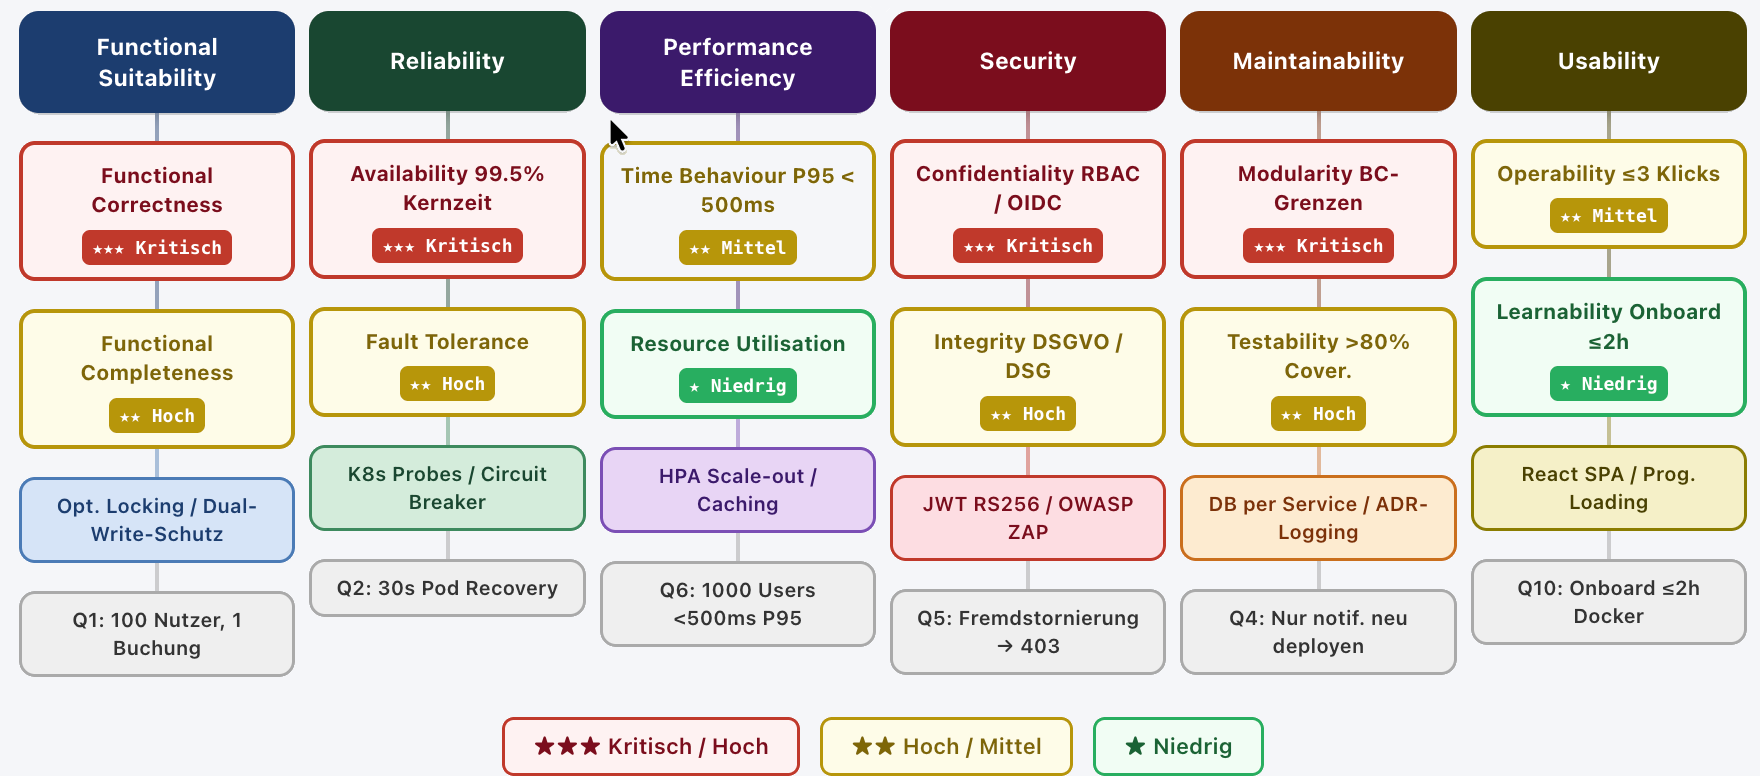
\includegraphics[width=0.95\linewidth]{assets/QualityTree}
  \caption{Grossansicht -- \textit{Qualitätsbaum: EduPlanner Qualitätsanforderungen}
    (vgl.\ Kap.~10.1, Abb.~\ref{fig:QualityTree})}
\end{figure}
\end{landscape}

% ── Risikobewertungsmatrix ───────────────────────────────────
\begin{landscape}
\begin{figure}[p]
  \centering
  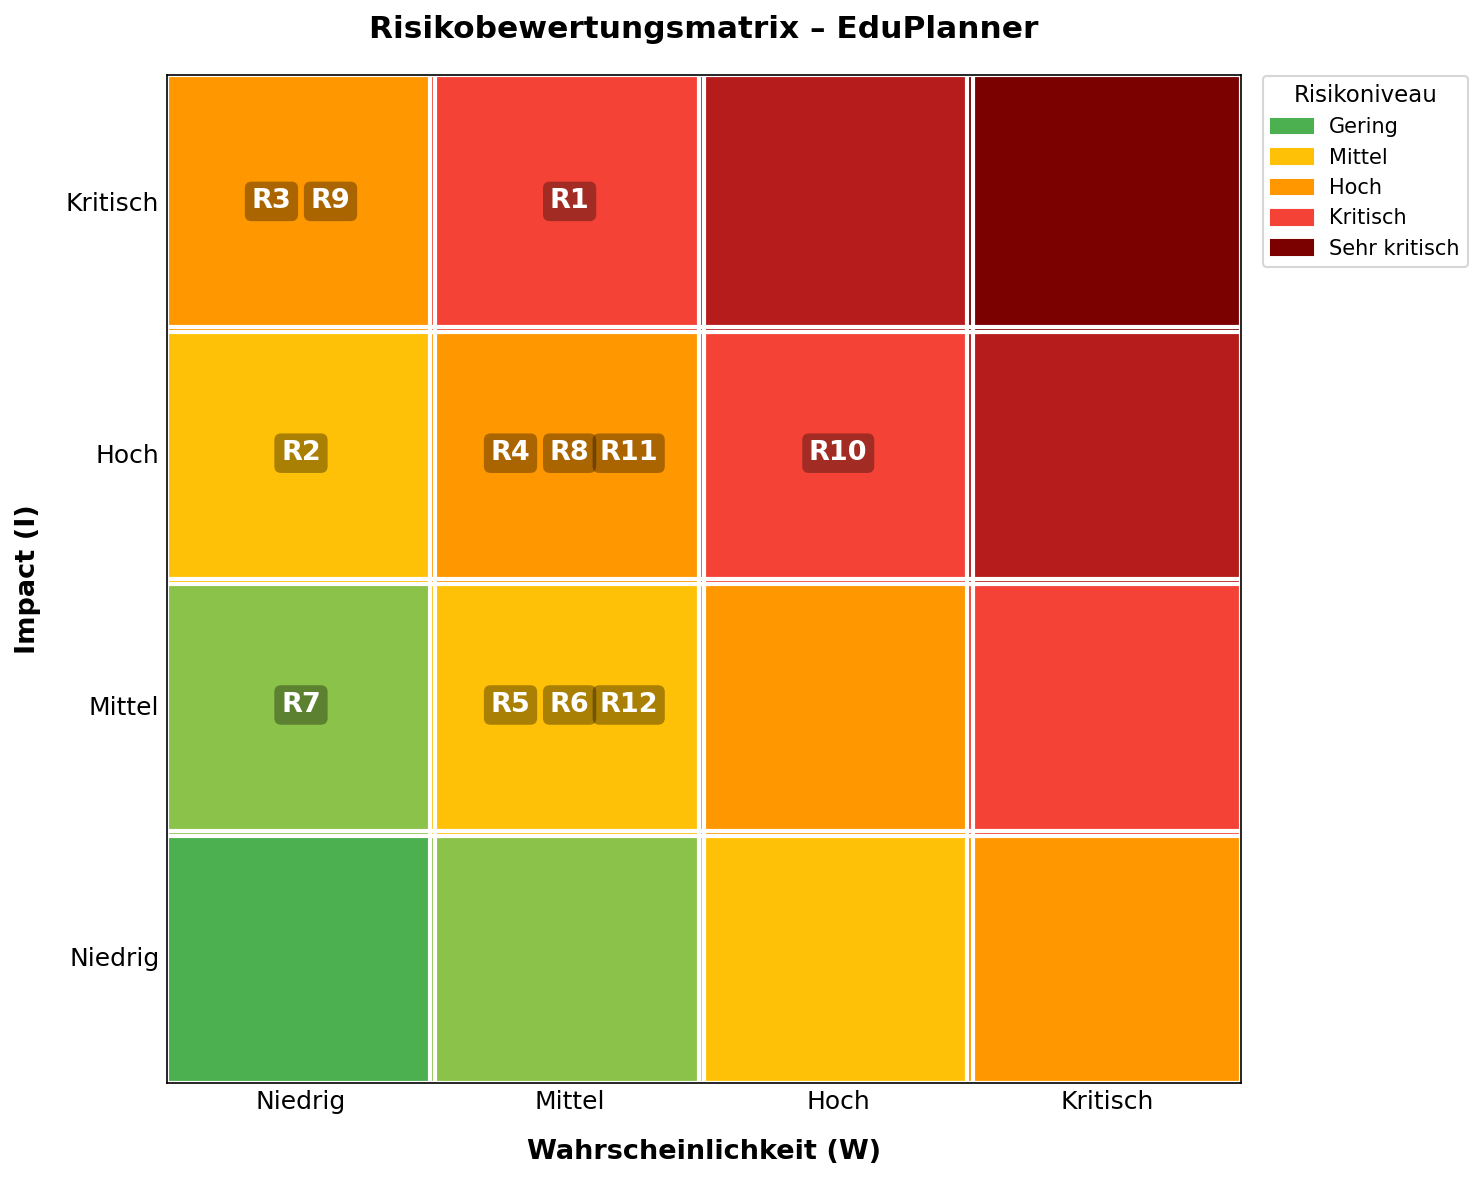
\includegraphics[width=0.85\linewidth]{assets/RiskMatrix}
  \caption{Grossansicht -- \textit{Risikobewertungsmatrix: Wahrscheinlichkeit vs.\ Impact (R1--R12)}
    (vgl.\ Kap.~11.1, Abb.~\ref{fig:RiskMatrix})}
\end{figure}
\end{landscape}

\newpage
% ============================================================
% ANHANG D – API-Referenz (OpenAPI 3.1.0 – Contract-First)
% ============================================================

\section{Anhang~D: API-Referenz}
\label{sec:anhang-openapi}

\begin{hinweis}[Contract-First -- Einzige Quelle der Wahrheit]
  Die Datei \texttt{openapi/}\allowbreak \texttt{eduplanner-}\allowbreak \texttt{api.yaml} ist die verbindliche
  API-Spezifikation (OpenAPI~3.1.0). Server-Stubs (Spring-Boot-Interfaces)
  werden daraus generiert -- nicht umgekehrt. Änderungen an der API
  \emph{beginnen immer} mit einer Änderung an der YAML-Datei.
  Begründung: ADR-011. Workflow: Kap.~8.4.
\end{hinweis}

% ── Contract-First Build-Pipeline ───────────────────────────
\subsection*{Contract-First Build-Pipeline}

\begin{figure}[H]
  \centering
  \begin{tabularx}{\textwidth}{C{0.6cm} L{3.8cm} X}
  \rowcolor{tableheader}
  \color{white}\textbf{\#} &
  \color{white}\textbf{Schritt} &
  \color{white}\textbf{Tool / Ergebnis} \\
  1 & Spec schreiben / ändern &
  \texttt{openapi/}\allowbreak \texttt{eduplanner-}\allowbreak \texttt{api.yaml} in Git committen \\
  \rowcolor{tablegrey}
  2 & Linting (CI) &
  \texttt{vacuum lint eduplanner-}\allowbreak \texttt{api.yaml} -- blockiert Build
  bei Verstössen gegen API-Design-Regeln \\
  3 & Server-Stubs generieren (Build) &
  \texttt{openapi-}\allowbreak \texttt{generator-}\allowbreak \texttt{maven-}\allowbreak \texttt{plugin} erzeugt
  Spring-Boot-Interfaces (\texttt{CoursesApi},
  \texttt{RegistrationsApi} etc.) mit
  \texttt{interfaceOnly=true} \\
  \rowcolor{tablegrey}
  4 & Implementieren &
  Dev-Team implementiert generierte Interfaces;
  Compiler erzwingt Konformität \\
  5 & Swagger~UI bereitstellen &
  \texttt{springdoc-}\allowbreak \texttt{openapi-}\allowbreak \texttt{starter-}\allowbreak \texttt{webmvc-}\allowbreak \texttt{ui} stellt
  \texttt{/swagger-ui/index.html} automatisch bereit \\
  \rowcolor{tablegrey}
  6 & Contract Tests (ab Sprint~8) &
  Pact-Tests validieren Consumer/Provider-Konformität
  (Tilgung TS2) \\
  \end{tabularx}
\end{figure}

\begin{hinweis}[Swagger~UI -- Zugriff je Umgebung]
  \begin{tabularx}{\textwidth}{L{3cm} X}
  \rowcolor{tableheader}
  \color{white}\textbf{Umgebung} & \color{white}\textbf{URL} \\
  Lokal (Docker) &
  \texttt{http://localhost:\{port\}/swagger-ui/index.html} \\
  \rowcolor{tablegrey}
  Staging &
  \texttt{https://staging-api.eduplanner.skillbridge.ch/}\allowbreak\texttt{\{service\}/swagger-ui/index.html} \\
  Produktion &
  Nur aus internem Netz (API-Gateway-Policy); nicht öffentlich erreichbar. \\
  \end{tabularx}
\end{hinweis}

% ── Endpunktübersicht ────────────────────────────────────────
\subsection*{Endpunktübersicht}

% ── Catalog ──────────────────────────────────────────────────
\begin{tabularx}{\textwidth}{L{1.3cm} L{5.8cm} L{2.3cm} X}
  \rowcolor{tableheader}
  \color{white}\textbf{Methode} &
  \color{white}\textbf{Pfad} &
  \color{white}\textbf{Service} &
  \color{white}\textbf{Mindestrolle} \\
  \multicolumn{4}{l}{\cellcolor{tablegrey}%
  \textbf{Catalog-Service} \small(\texttt{/swagger-ui/index.html}, Port~8081)} \\
  GET    & \texttt{/courses}                      & catalog & Authentifiziert \\
  \rowcolor{tablegrey}
  POST   & \texttt{/courses}                      & catalog & STAFF \\
  GET    & \texttt{/courses/\{courseId\}}         & catalog & Authentifiziert \\
  \rowcolor{tablegrey}
  PUT    & \texttt{/courses/\{courseId\}}         & catalog & STAFF \\
  DELETE & \texttt{/courses/\{courseId\}}         & catalog & ADMIN \\
  \rowcolor{tablegrey}
  PUT    & \texttt{/courses/\{courseId\}/publish} & catalog & ADMIN \\
  PUT    & \texttt{/courses/\{courseId\}/archive} & catalog & ADMIN \\
  \rowcolor{tablegrey}
  GET    & \texttt{/trainers}                     & catalog & Authentifiziert \\
  POST   & \texttt{/trainers}                     & catalog & STAFF \\
  \rowcolor{tablegrey}
  GET    & \texttt{/trainers/\{trainerId\}}       & catalog & Authentifiziert \\
  PUT    & \texttt{/trainers/\{trainerId\}}       & catalog & STAFF \\
\end{tabularx}

\vspace{0.8em}

% ── Scheduling ───────────────────────────────────────────────
\begin{tabularx}{\textwidth}{L{1.3cm} L{5.8cm} L{2.3cm} X}
  \rowcolor{tableheader}
  \color{white}\textbf{Methode} &
  \color{white}\textbf{Pfad} &
  \color{white}\textbf{Service} &
  \color{white}\textbf{Mindestrolle} \\
  \multicolumn{4}{l}{\cellcolor{tablegrey}%
  \textbf{Scheduling-Service} \small(\texttt{/swagger-ui/index.html}, Port~8082)} \\
  GET    & \texttt{/executions}                          & scheduling & Authentifiziert \\
  \rowcolor{tablegrey}
  POST   & \texttt{/executions}                          & scheduling & STAFF \\
  GET    & \texttt{/executions/\{executionId\}}          & scheduling & Authentifiziert \\
  \rowcolor{tablegrey}
  PUT    & \texttt{/executions/\{executionId\}}          & scheduling & STAFF \\
  PUT    & \texttt{/executions/\{executionId\} /publish}  & scheduling & ADMIN \\
  \rowcolor{tablegrey}
  PUT    & \texttt{/executions/\{executionId\} /cancel}   & scheduling & ADMIN \\
  GET    & \texttt{/executions/\{executionId\} /participants} & scheduling & STAFF \\
\end{tabularx}

\vspace{0.8em}

% ── Registration ─────────────────────────────────────────────
\begin{tabularx}{\textwidth}{L{1.3cm} L{5.8cm} L{2.3cm} X}
  \rowcolor{tableheader}
  \color{white}\textbf{Methode} &
  \color{white}\textbf{Pfad} &
  \color{white}\textbf{Service} &
  \color{white}\textbf{Mindestrolle} \\
  \multicolumn{4}{l}{\cellcolor{tablegrey}%
  \textbf{Registration-Service} \small(\texttt{/swagger-ui/index.html}, Port~8083 -- kritischster Service)} \\
  GET    & \texttt{/registrations}                        & registration & Authentifiziert \\
  \rowcolor{tablegrey}
  POST   & \texttt{/registrations}                        & registration & PARTICIPANT \\
  GET    & \texttt{/registrations/\{id\}}                 & registration & Authentifiziert \\
  \rowcolor{tablegrey}
  DELETE & \texttt{/registrations/\{id\}}                 & registration & PARTICIPANT \\
  GET    & \texttt{/registrations/\{id\} /waitlist-position} & registration & Authentifiziert \\
\end{tabularx}

\vspace{0.8em}

% ── Identity ─────────────────────────────────────────────────
\begin{tabularx}{\textwidth}{L{1.3cm} L{5.8cm} L{2.3cm} X}
  \rowcolor{tableheader}
  \color{white}\textbf{Methode} &
  \color{white}\textbf{Pfad} &
  \color{white}\textbf{Service} &
  \color{white}\textbf{Mindestrolle} \\
  \multicolumn{4}{l}{\cellcolor{tablegrey}%
  \textbf{Identity-Service} \small(\texttt{/swagger-ui/index.html}, Port~8084)} \\
  GET    & \texttt{/users}                    & identity & ADMIN \\
  \rowcolor{tablegrey}
  GET    & \texttt{/users/\{userId\}}         & identity & ADMIN\,/\,eigenes Profil \\
  GET    & \texttt{/users/\{userId\}/roles}   & identity & ADMIN \\
  \rowcolor{tablegrey}
  PUT    & \texttt{/users/\{userId\}/roles}   & identity & ADMIN \\
  DELETE & \texttt{/users/\{userId\}/delete-pii} & identity & ADMIN \\
  \rowcolor{tablegrey}
  GET    & \texttt{/me}                       & identity & Authentifiziert \\
\end{tabularx}

% ── Designentscheide aus der Spec ───────────────────────────
\subsection*{Designentscheide}

\begin{tabularx}{\textwidth}{L{3.5cm} X}
  \rowcolor{tableheader}
  \color{white}\textbf{Aspekt} & \color{white}\textbf{Umsetzung} \\
  Authentifizierung & RS256-signierter JWT Bearer Token; 15~Min.\ Laufzeit;
  Validierung am API Gateway (Kap.~8.1). \\
  \rowcolor{tablegrey}
  Fehlerantworten & RFC~7807 \texttt{application/problem+json} mit
  \texttt{type}, \texttt{title}, \texttt{status}, \texttt{detail},
  \texttt{instance}, \texttt{errors} (Kap.~8.4). \\
  Pagination & Cursor-basiert (\texttt{?cursor=\ldots\&limit=20},
  max.\ 100); kein Offset-Paging. \\
  \rowcolor{tablegrey}
  Idempotency & \texttt{Idempotency-Key}-Header (UUID) bei allen
  POST-Endpunkten (Kap.~5.4). \\
  Kapazitätsprüfung & \texttt{POST /registrations}: 201~Created bei
  freiem Platz; 202~Accepted auf Warteliste (Kap.~6.1, 6.2). \\
  \rowcolor{tablegrey}
  DSGVO-Löschung & \texttt{DELETE /users/\{id\}/delete-pii}: 202~Accepted,
  Abschluss innerhalb 30~Tagen (Q8, Q12). \\
  Versionierung & \texttt{/api/v1/...}; Breaking Changes $\to$
  \texttt{/api/v2/...} (ADR-011). \\
  \rowcolor{tablegrey}
  PII-Schutz & \texttt{User}-Schema enthält keine E-Mail-Adresse;
  nur \texttt{userId} (UUID) in Events (Kap.~8.2, 4.3). \\
  Optimistic Locking & \texttt{version}-Feld (int64) in
  \texttt{Course}, \texttt{CourseExecution}, \texttt{Registration};
  Konflikt $\to$ 409~Conflict (Kap.~8.3). \\
\end{tabularx}

\newpage
\printbibliography[title={Literaturverzeichnis}, heading=bibintoc]

\end{document}
